% Options for packages loaded elsewhere
\PassOptionsToPackage{unicode}{hyperref}
\PassOptionsToPackage{hyphens}{url}
%
\documentclass[
  doc,floatsintext]{apa6}
\usepackage{amsmath,amssymb}
\usepackage{iftex}
\ifPDFTeX
  \usepackage[T1]{fontenc}
  \usepackage[utf8]{inputenc}
  \usepackage{textcomp} % provide euro and other symbols
\else % if luatex or xetex
  \usepackage{unicode-math} % this also loads fontspec
  \defaultfontfeatures{Scale=MatchLowercase}
  \defaultfontfeatures[\rmfamily]{Ligatures=TeX,Scale=1}
\fi
\usepackage{lmodern}
\ifPDFTeX\else
  % xetex/luatex font selection
\fi
% Use upquote if available, for straight quotes in verbatim environments
\IfFileExists{upquote.sty}{\usepackage{upquote}}{}
\IfFileExists{microtype.sty}{% use microtype if available
  \usepackage[]{microtype}
  \UseMicrotypeSet[protrusion]{basicmath} % disable protrusion for tt fonts
}{}
\makeatletter
\@ifundefined{KOMAClassName}{% if non-KOMA class
  \IfFileExists{parskip.sty}{%
    \usepackage{parskip}
  }{% else
    \setlength{\parindent}{0pt}
    \setlength{\parskip}{6pt plus 2pt minus 1pt}}
}{% if KOMA class
  \KOMAoptions{parskip=half}}
\makeatother
\usepackage{xcolor}
\usepackage{color}
\usepackage{fancyvrb}
\newcommand{\VerbBar}{|}
\newcommand{\VERB}{\Verb[commandchars=\\\{\}]}
\DefineVerbatimEnvironment{Highlighting}{Verbatim}{commandchars=\\\{\}}
% Add ',fontsize=\small' for more characters per line
\usepackage{framed}
\definecolor{shadecolor}{RGB}{248,248,248}
\newenvironment{Shaded}{\begin{snugshade}}{\end{snugshade}}
\newcommand{\AlertTok}[1]{\textcolor[rgb]{0.94,0.16,0.16}{#1}}
\newcommand{\AnnotationTok}[1]{\textcolor[rgb]{0.56,0.35,0.01}{\textbf{\textit{#1}}}}
\newcommand{\AttributeTok}[1]{\textcolor[rgb]{0.13,0.29,0.53}{#1}}
\newcommand{\BaseNTok}[1]{\textcolor[rgb]{0.00,0.00,0.81}{#1}}
\newcommand{\BuiltInTok}[1]{#1}
\newcommand{\CharTok}[1]{\textcolor[rgb]{0.31,0.60,0.02}{#1}}
\newcommand{\CommentTok}[1]{\textcolor[rgb]{0.56,0.35,0.01}{\textit{#1}}}
\newcommand{\CommentVarTok}[1]{\textcolor[rgb]{0.56,0.35,0.01}{\textbf{\textit{#1}}}}
\newcommand{\ConstantTok}[1]{\textcolor[rgb]{0.56,0.35,0.01}{#1}}
\newcommand{\ControlFlowTok}[1]{\textcolor[rgb]{0.13,0.29,0.53}{\textbf{#1}}}
\newcommand{\DataTypeTok}[1]{\textcolor[rgb]{0.13,0.29,0.53}{#1}}
\newcommand{\DecValTok}[1]{\textcolor[rgb]{0.00,0.00,0.81}{#1}}
\newcommand{\DocumentationTok}[1]{\textcolor[rgb]{0.56,0.35,0.01}{\textbf{\textit{#1}}}}
\newcommand{\ErrorTok}[1]{\textcolor[rgb]{0.64,0.00,0.00}{\textbf{#1}}}
\newcommand{\ExtensionTok}[1]{#1}
\newcommand{\FloatTok}[1]{\textcolor[rgb]{0.00,0.00,0.81}{#1}}
\newcommand{\FunctionTok}[1]{\textcolor[rgb]{0.13,0.29,0.53}{\textbf{#1}}}
\newcommand{\ImportTok}[1]{#1}
\newcommand{\InformationTok}[1]{\textcolor[rgb]{0.56,0.35,0.01}{\textbf{\textit{#1}}}}
\newcommand{\KeywordTok}[1]{\textcolor[rgb]{0.13,0.29,0.53}{\textbf{#1}}}
\newcommand{\NormalTok}[1]{#1}
\newcommand{\OperatorTok}[1]{\textcolor[rgb]{0.81,0.36,0.00}{\textbf{#1}}}
\newcommand{\OtherTok}[1]{\textcolor[rgb]{0.56,0.35,0.01}{#1}}
\newcommand{\PreprocessorTok}[1]{\textcolor[rgb]{0.56,0.35,0.01}{\textit{#1}}}
\newcommand{\RegionMarkerTok}[1]{#1}
\newcommand{\SpecialCharTok}[1]{\textcolor[rgb]{0.81,0.36,0.00}{\textbf{#1}}}
\newcommand{\SpecialStringTok}[1]{\textcolor[rgb]{0.31,0.60,0.02}{#1}}
\newcommand{\StringTok}[1]{\textcolor[rgb]{0.31,0.60,0.02}{#1}}
\newcommand{\VariableTok}[1]{\textcolor[rgb]{0.00,0.00,0.00}{#1}}
\newcommand{\VerbatimStringTok}[1]{\textcolor[rgb]{0.31,0.60,0.02}{#1}}
\newcommand{\WarningTok}[1]{\textcolor[rgb]{0.56,0.35,0.01}{\textbf{\textit{#1}}}}
\usepackage{graphicx}
\makeatletter
\def\maxwidth{\ifdim\Gin@nat@width>\linewidth\linewidth\else\Gin@nat@width\fi}
\def\maxheight{\ifdim\Gin@nat@height>\textheight\textheight\else\Gin@nat@height\fi}
\makeatother
% Scale images if necessary, so that they will not overflow the page
% margins by default, and it is still possible to overwrite the defaults
% using explicit options in \includegraphics[width, height, ...]{}
\setkeys{Gin}{width=\maxwidth,height=\maxheight,keepaspectratio}
% Set default figure placement to htbp
\makeatletter
\def\fps@figure{htbp}
\makeatother
\setlength{\emergencystretch}{3em} % prevent overfull lines
\providecommand{\tightlist}{%
  \setlength{\itemsep}{0pt}\setlength{\parskip}{0pt}}
\setcounter{secnumdepth}{-\maxdimen} % remove section numbering
% Make \paragraph and \subparagraph free-standing
\makeatletter
\ifx\paragraph\undefined\else
  \let\oldparagraph\paragraph
  \renewcommand{\paragraph}{
    \@ifstar
      \xxxParagraphStar
      \xxxParagraphNoStar
  }
  \newcommand{\xxxParagraphStar}[1]{\oldparagraph*{#1}\mbox{}}
  \newcommand{\xxxParagraphNoStar}[1]{\oldparagraph{#1}\mbox{}}
\fi
\ifx\subparagraph\undefined\else
  \let\oldsubparagraph\subparagraph
  \renewcommand{\subparagraph}{
    \@ifstar
      \xxxSubParagraphStar
      \xxxSubParagraphNoStar
  }
  \newcommand{\xxxSubParagraphStar}[1]{\oldsubparagraph*{#1}\mbox{}}
  \newcommand{\xxxSubParagraphNoStar}[1]{\oldsubparagraph{#1}\mbox{}}
\fi
\makeatother
\ifLuaTeX
\usepackage[bidi=basic]{babel}
\else
\usepackage[bidi=default]{babel}
\fi
\babelprovide[main,import]{english}
% get rid of language-specific shorthands (see #6817):
\let\LanguageShortHands\languageshorthands
\def\languageshorthands#1{}
% Manuscript styling
\usepackage{upgreek}
\captionsetup{font=singlespacing,justification=justified}

% Table formatting
\usepackage{longtable}
\usepackage{lscape}
% \usepackage[counterclockwise]{rotating}   % Landscape page setup for large tables
\usepackage{multirow}		% Table styling
\usepackage{tabularx}		% Control Column width
\usepackage[flushleft]{threeparttable}	% Allows for three part tables with a specified notes section
\usepackage{threeparttablex}            % Lets threeparttable work with longtable

% Create new environments so endfloat can handle them
% \newenvironment{ltable}
%   {\begin{landscape}\centering\begin{threeparttable}}
%   {\end{threeparttable}\end{landscape}}
\newenvironment{lltable}{\begin{landscape}\centering\begin{ThreePartTable}}{\end{ThreePartTable}\end{landscape}}

% Enables adjusting longtable caption width to table width
% Solution found at http://golatex.de/longtable-mit-caption-so-breit-wie-die-tabelle-t15767.html
\makeatletter
\newcommand\LastLTentrywidth{1em}
\newlength\longtablewidth
\setlength{\longtablewidth}{1in}
\newcommand{\getlongtablewidth}{\begingroup \ifcsname LT@\roman{LT@tables}\endcsname \global\longtablewidth=0pt \renewcommand{\LT@entry}[2]{\global\advance\longtablewidth by ##2\relax\gdef\LastLTentrywidth{##2}}\@nameuse{LT@\roman{LT@tables}} \fi \endgroup}

% \setlength{\parindent}{0.5in}
% \setlength{\parskip}{0pt plus 0pt minus 0pt}

% Overwrite redefinition of paragraph and subparagraph by the default LaTeX template
% See https://github.com/crsh/papaja/issues/292
\makeatletter
\renewcommand{\paragraph}{\@startsection{paragraph}{4}{\parindent}%
  {0\baselineskip \@plus 0.2ex \@minus 0.2ex}%
  {-1em}%
  {\normalfont\normalsize\bfseries\itshape\typesectitle}}

\renewcommand{\subparagraph}[1]{\@startsection{subparagraph}{5}{1em}%
  {0\baselineskip \@plus 0.2ex \@minus 0.2ex}%
  {-\z@\relax}%
  {\normalfont\normalsize\itshape\hspace{\parindent}{#1}\textit{\addperi}}{\relax}}
\makeatother

\makeatletter
\usepackage{etoolbox}
\patchcmd{\maketitle}
  {\section{\normalfont\normalsize\abstractname}}
  {\section*{\normalfont\normalsize\abstractname}}
  {}{\typeout{Failed to patch abstract.}}
\patchcmd{\maketitle}
  {\section{\protect\normalfont{\@title}}}
  {\section*{\protect\normalfont{\@title}}}
  {}{\typeout{Failed to patch title.}}
\makeatother

\usepackage{xpatch}
\makeatletter
\xapptocmd\appendix
  {\xapptocmd\section
    {\addcontentsline{toc}{section}{\appendixname\ifoneappendix\else~\theappendix\fi\\: #1}}
    {}{\InnerPatchFailed}%
  }
{}{\PatchFailed}
\usepackage{lineno}

\linenumbers
\usepackage{csquotes}
\ifLuaTeX
  \usepackage{selnolig}  % disable illegal ligatures
\fi
\usepackage{bookmark}
\IfFileExists{xurl.sty}{\usepackage{xurl}}{} % add URL line breaks if available
\urlstyle{same}
\hypersetup{
  pdftitle={Exp. 1 Revised Analysis},
  pdflang={en-EN},
  hidelinks,
  pdfcreator={LaTeX via pandoc}}

\title{Exp. 1 Revised Analysis}
\author{\phantom{0}}
\date{}


\shorttitle{Revised Exp 1}

\affiliation{\phantom{0}}

\begin{document}
\maketitle

\subsection{Reviewer 2}\label{reviewer-2}

\begin{quote}
There is another concern about the data analysis that I'd like to raise. The trial-level inclusion criterion of a minimum of 500 ms during the analysis window seems extremely liberal, particularly since the window is 3500 ms long.
\end{quote}

\begin{quote}
However, a subsequent PNAS paper by Bergelson \& Aslin (2017), also cited in the manuscript, used a more conservative criterion: `Trials were excluded if infants did not look at either image for at least 1/3 of the target window'. This 1/3 criterion was also used by Bergelson \& Swingley (2017). The 1/3 choice seems like a much more reasonable inclusion criterion than the 1/7 used in the current study, which seems like it could lead to a lot of noise.
\end{quote}

\begin{quote}
It is also standard to exclude infants who do not provide data for at least half of the test trials (cf.~Bergelson \& Swingley, 2017). I understand that this is a very difficult-to-test sample, and that the authors want to retain as many infants in the sample as possible, but there is a tradeoff between data retention and interpretability of the effects. In particular, the 1/7 data retention criterion seems quite problematic.
\end{quote}

\subsection{Adopting (3133/3)ms looking-time threshhold for trial inclusion}\label{adopting-31333ms-looking-time-threshhold-for-trial-inclusion}

\begin{Shaded}
\begin{Highlighting}[]
\DocumentationTok{\#\# exclusions}
\NormalTok{cn\_r2}\SpecialCharTok{$}\NormalTok{exclusions }\OtherTok{\textless{}{-}}\NormalTok{ cn\_r2}\SpecialCharTok{$}\NormalTok{keep}
\NormalTok{cn\_r2}\SpecialCharTok{$}\NormalTok{exclusions[cn\_r2}\SpecialCharTok{$}\NormalTok{keep}\SpecialCharTok{==}\StringTok{\textquotesingle{}keep\textquotesingle{}}\NormalTok{] }\OtherTok{\textless{}{-}} \StringTok{\textquotesingle{}\textquotesingle{}}
\NormalTok{cn\_r2}\SpecialCharTok{$}\NormalTok{exclusions[cn\_r2}\SpecialCharTok{$}\NormalTok{exclusions }\SpecialCharTok{\%in\%} \FunctionTok{c}\NormalTok{(}
  \StringTok{\textquotesingle{}infant not paying attention\textquotesingle{}}\NormalTok{, }\StringTok{\textquotesingle{}infant crying\textquotesingle{}}\NormalTok{)] }\OtherTok{\textless{}{-}} 
  \StringTok{\textquotesingle{}restive\_infant\textquotesingle{}}
\NormalTok{cn\_r2}\SpecialCharTok{$}\NormalTok{exclusions[cn\_r2}\SpecialCharTok{$}\NormalTok{pre\_looking\_sum\_ms }\SpecialCharTok{==} \DecValTok{0}\NormalTok{] }\OtherTok{\textless{}{-}}
  \StringTok{\textquotesingle{}zero\_pre\_looking\textquotesingle{}}
\NormalTok{cn\_r2}\SpecialCharTok{$}\NormalTok{exclusions[cn\_r2}\SpecialCharTok{$}\NormalTok{post1\_looking\_sum\_ms }\SpecialCharTok{\textless{}}\NormalTok{ (}\DecValTok{3133}\SpecialCharTok{/}\DecValTok{3}\NormalTok{)] }\OtherTok{\textless{}{-}}
  \StringTok{\textquotesingle{}under\_third\_window\_looking\textquotesingle{}}
\NormalTok{cn\_r2}\SpecialCharTok{$}\NormalTok{exclusions[cn\_r2}\SpecialCharTok{$}\NormalTok{exclusions}\SpecialCharTok{==}\StringTok{\textquotesingle{}mom\_interference\textquotesingle{}}\NormalTok{] }\OtherTok{\textless{}{-}}
  \StringTok{\textquotesingle{}mom\_error\textquotesingle{}}
\NormalTok{cn\_r2}\SpecialCharTok{$}\NormalTok{exclusions[cn\_r2}\SpecialCharTok{$}\NormalTok{exclusions}\SpecialCharTok{==}\StringTok{\textquotesingle{}discard\textquotesingle{}}\NormalTok{] }\OtherTok{\textless{}{-}}
  \StringTok{\textquotesingle{}\textquotesingle{}}
\NormalTok{TOTAL\_EXCLUDED\_TRIALS }\OtherTok{\textless{}{-}} \FunctionTok{nrow}\NormalTok{(cn\_r2[cn\_r2}\SpecialCharTok{$}\NormalTok{exclusions }\SpecialCharTok{\%in\%} 
                                      \FunctionTok{c}\NormalTok{(}\StringTok{\textquotesingle{}restive\_infant\textquotesingle{}}\NormalTok{, }\StringTok{\textquotesingle{}zero\_pre\_looking\textquotesingle{}}\NormalTok{, }
                                        \StringTok{\textquotesingle{}mom\_error\textquotesingle{}}\NormalTok{,}
                                        \StringTok{\textquotesingle{}under\_third\_window\_looking\textquotesingle{}}\NormalTok{),]) }
\SpecialCharTok{+} \DecValTok{3} \CommentTok{\# mom\_errors flagged in Datavyu export script:}
\end{Highlighting}
\end{Shaded}

\begin{verbatim}
## [1] 3
\end{verbatim}

\begin{Shaded}
\begin{Highlighting}[]
\CommentTok{\# \textquotesingle{}Invalid number of wordWindow cells\textquotesingle{} (because of mom not speaking prompt)\textquotesingle{} }
\end{Highlighting}
\end{Shaded}

\begin{Shaded}
\begin{Highlighting}[]
\NormalTok{cn\_exclusions\_tab }\OtherTok{\textless{}{-}}\NormalTok{ cn\_r2 }\SpecialCharTok{\%\textgreater{}\%}
  \FunctionTok{filter}\NormalTok{(exclusions}\SpecialCharTok{!=}\StringTok{\textquotesingle{}trial\_was\_recycled\textquotesingle{}}\NormalTok{,}
\NormalTok{         exclusions}\SpecialCharTok{!=}\StringTok{\textquotesingle{}old\_trial\_type\textquotesingle{}}\NormalTok{) }\SpecialCharTok{\%\textgreater{}\%}
  \FunctionTok{group\_by}\NormalTok{(subject\_id) }\SpecialCharTok{\%\textgreater{}\%}
  \FunctionTok{summarize}\NormalTok{(}\AttributeTok{excluded\_trials=}\FunctionTok{sum}\NormalTok{(exclusions}\SpecialCharTok{!=}\StringTok{\textquotesingle{}\textquotesingle{}}\NormalTok{)) }\SpecialCharTok{\%\textgreater{}\%}
  \FunctionTok{ungroup}\NormalTok{() }\SpecialCharTok{\%\textgreater{}\%}
  \FunctionTok{summarize}\NormalTok{(}\AttributeTok{children\_w\_excl\_trials=}\FunctionTok{sum}\NormalTok{(excluded\_trials}\SpecialCharTok{\textgreater{}}\DecValTok{0}\NormalTok{),}
            \AttributeTok{min\_excl\_trials=}\FunctionTok{min}\NormalTok{(excluded\_trials),}
            \AttributeTok{max\_excl\_trials=}\FunctionTok{max}\NormalTok{(excluded\_trials),}
            \AttributeTok{mean\_excl\_trials=}\FunctionTok{mean}\NormalTok{(excluded\_trials))}

\FunctionTok{xtable2kable}\NormalTok{(cn\_exclusions\_tab)}
\end{Highlighting}
\end{Shaded}

\begin{verbatim}
## # A tibble: 1 x 4
##   children_w_excl_trials min_excl_trials max_excl_trials mean_excl_trials
##                    <int>           <int>           <int>            <dbl>
## 1                     20               0              16             4.52
\end{verbatim}

Excluded test trials came from 20 infants who had between 0 and 16 excluded trials; all infants provided usable data for at least half of the test trials. If we instead adopt the criteria that infants should provide data for at least half of the difference score calculations, then one subject (`J94252'), with 16 test trials, but only two calculable difference scores, should be excluded (see next section---`EXCLUSION CRITERIA 2'---for revised mean difference score analyses, which use this criterion).

\begin{Shaded}
\begin{Highlighting}[]
\NormalTok{cn\_keeptrials\_tab }\OtherTok{\textless{}{-}}\NormalTok{ cn\_r2 }\SpecialCharTok{\%\textgreater{}\%}
  \FunctionTok{group\_by}\NormalTok{(subject\_id) }\SpecialCharTok{\%\textgreater{}\%}
  \FunctionTok{summarize}\NormalTok{(}\AttributeTok{good\_sum=}\FunctionTok{sum}\NormalTok{(exclusions}\SpecialCharTok{==}\StringTok{\textquotesingle{}\textquotesingle{}}\NormalTok{),}
            \AttributeTok{good\_prop =}\NormalTok{ good\_sum}\SpecialCharTok{/}\FunctionTok{n}\NormalTok{(),}
            \AttributeTok{good\_prop\_of\_total =}\NormalTok{ good\_sum}\SpecialCharTok{/}\DecValTok{32}\NormalTok{) }\SpecialCharTok{\%\textgreater{}\%}
  \FunctionTok{ungroup}\NormalTok{() }\SpecialCharTok{\%\textgreater{}\%}
  \FunctionTok{reframe}\NormalTok{(}\AttributeTok{min\_good\_trials=}\FunctionTok{min}\NormalTok{(good\_sum),}
            \AttributeTok{min\_n=}\FunctionTok{sum}\NormalTok{(good\_sum}\SpecialCharTok{==}\NormalTok{min\_good\_trials),}
            \AttributeTok{max\_good\_trials=}\FunctionTok{max}\NormalTok{(good\_sum),}
            \AttributeTok{max\_n=}\FunctionTok{sum}\NormalTok{(good\_sum}\SpecialCharTok{==}\NormalTok{max\_good\_trials),}
            \AttributeTok{mean\_good\_trials=}\FunctionTok{mean}\NormalTok{(good\_sum),}
            \AttributeTok{med =} \FunctionTok{median}\NormalTok{(good\_sum),}
            \AttributeTok{mode\_good\_trials=}\NormalTok{DescTools}\SpecialCharTok{::}\FunctionTok{Mode}\NormalTok{(good\_sum),}
            \AttributeTok{mode\_n=}\FunctionTok{sum}\NormalTok{(good\_sum}\SpecialCharTok{==}\NormalTok{mode\_good\_trials),}
            \AttributeTok{min\_good\_prop =} \FunctionTok{min}\NormalTok{(good\_prop\_of\_total),}
            \AttributeTok{max\_good\_prop=}\FunctionTok{max}\NormalTok{(good\_prop\_of\_total),}
            \AttributeTok{mean\_good\_prop=}\FunctionTok{mean}\NormalTok{(good\_prop\_of\_total)) }\SpecialCharTok{\%\textgreater{}\%}
  \FunctionTok{round}\NormalTok{(., }\DecValTok{2}\NormalTok{)}

\FunctionTok{xtable2kable}\NormalTok{(cn\_keeptrials\_tab)}
\end{Highlighting}
\end{Shaded}

\begin{verbatim}
## # A tibble: 3 x 11
##   min_good_trials min_n max_good_trials max_n mean_good_trials   med
##             <dbl> <dbl>           <dbl> <dbl>            <dbl> <dbl>
## 1              16     3              32     1             25.1    26
## 2              16     3              32     1             25.1    26
## 3              16     3              32     1             25.1    26
## # i 5 more variables: mode_good_trials <dbl>, mode_n <dbl>,
## #   min_good_prop <dbl>, max_good_prop <dbl>, mean_good_prop <dbl>
\end{verbatim}

A total of \(93\) trials from 20 infants were excluded because the infant never looked to the displays during the pre-naming period (\(n=14\)), looked for less than one-third of the analysis window (\(n=72\)), was distracted or crying (\(n=3\)), or because the caregiver erred or interfered (\(n=7\)). All infants contributed at least half (16) of test trials (\textit{range}\(=c(16, 16, 16)-c(32, 32, 32)\), \(M_\textnormal{trials}=c(25.14, 25.14, 25.14)\), \(Med_\textnormal{trials}=c(26, 26, 26)\)).

\section{EXCLUSION CRITERIA 1}\label{exclusion-criteria-1}

\begin{Shaded}
\begin{Highlighting}[]
\NormalTok{cn\_fin }\OtherTok{\textless{}{-}}\NormalTok{ cn\_r2 }\SpecialCharTok{\%\textgreater{}\%} \FunctionTok{filter}\NormalTok{(exclusions}\SpecialCharTok{==}\StringTok{\textquotesingle{}\textquotesingle{}}\NormalTok{)}
\FunctionTok{write.csv}\NormalTok{(cn\_fin,}
          \FunctionTok{here}\NormalTok{(}\StringTok{\textquotesingle{}data/common\_nouns\_reviewer2\_data.csv\textquotesingle{}}\NormalTok{))}

\NormalTok{cn\_fin\_pp\_df }\OtherTok{\textless{}{-}}\NormalTok{ cn\_fin }\SpecialCharTok{\%\textgreater{}\%}
  \FunctionTok{distinct}\NormalTok{(subject\_id, bebe\_meses, mama\_edad) }

\NormalTok{N }\OtherTok{\textless{}{-}} \FunctionTok{length}\NormalTok{(}\FunctionTok{unique}\NormalTok{(cn\_fin\_pp\_df}\SpecialCharTok{$}\NormalTok{subject\_id))}
\NormalTok{MIN\_AGE }\OtherTok{\textless{}{-}} \FunctionTok{min}\NormalTok{(cn\_fin\_pp\_df}\SpecialCharTok{$}\NormalTok{bebe\_meses)}
\NormalTok{MAX\_AGE }\OtherTok{\textless{}{-}} \FunctionTok{max}\NormalTok{(cn\_fin\_pp\_df}\SpecialCharTok{$}\NormalTok{bebe\_meses)}
\NormalTok{MEAN\_AGE }\OtherTok{\textless{}{-}} \FunctionTok{mean}\NormalTok{(cn\_fin\_pp\_df}\SpecialCharTok{$}\NormalTok{bebe\_meses)}
\NormalTok{SD\_AGE }\OtherTok{\textless{}{-}} \FunctionTok{sd}\NormalTok{(cn\_fin\_pp\_df}\SpecialCharTok{$}\NormalTok{bebe\_meses)}
\end{Highlighting}
\end{Shaded}

We report on data from \(21\) infants (\(5.33-15.43\)\textit{mos}, \(M_\textnormal{age}=10.96\)\textit{mos}, \(SD_\textnormal{age}=2.71\)\textit{mos}).

\begin{Shaded}
\begin{Highlighting}[]
\NormalTok{MOT\_M\_AGE }\OtherTok{\textless{}{-}} \FunctionTok{na.mean}\NormalTok{(cn\_fin\_pp\_df}\SpecialCharTok{$}\NormalTok{mama\_edad)}
\NormalTok{MOT\_MIN\_AGE }\OtherTok{\textless{}{-}} \FunctionTok{min}\NormalTok{(cn\_fin\_pp\_df}\SpecialCharTok{$}\NormalTok{mama\_edad, }\AttributeTok{na.rm=}\NormalTok{T)}
\NormalTok{MOT\_MAX\_AGE }\OtherTok{\textless{}{-}} \FunctionTok{max}\NormalTok{(cn\_fin\_pp\_df}\SpecialCharTok{$}\NormalTok{mama\_edad, }\AttributeTok{na.rm=}\NormalTok{T)}
\NormalTok{MOT\_SD\_AGE }\OtherTok{\textless{}{-}} \FunctionTok{sd}\NormalTok{(cn\_fin\_pp\_df}\SpecialCharTok{$}\NormalTok{mama\_edad, }\AttributeTok{na.rm=}\NormalTok{T)}
\end{Highlighting}
\end{Shaded}

Mothers ranged in age from \(14\) to \(44\)\textit{yrs} (\(M_\textnormal{age}=26.85\)\textit{yrs}, \(SD_\textnormal{age}=8.36\)\textit{yrs})

\subsection{Mean Difference Score Analysis}\label{mean-difference-score-analysis}

\begin{Shaded}
\begin{Highlighting}[]
\DocumentationTok{\#\# specific image pairs (which of two image{-}pairs for each noun{-}pair)}
\CommentTok{\# want to know the pairs of values that go together for the B\&S 2012 calculation,}
\CommentTok{\# which means the specific instances of each noun{-}pair where, e.g., baby is on L}
\CommentTok{\# and corn is on R}
\NormalTok{cn\_fin}\SpecialCharTok{$}\NormalTok{trial\_name\_short }\OtherTok{\textless{}{-}} \FunctionTok{gsub}\NormalTok{(}\StringTok{\textquotesingle{}\^{}[0{-}9]*[{-}]\textquotesingle{}}\NormalTok{, }\StringTok{\textquotesingle{}\textquotesingle{}}\NormalTok{, cn\_fin}\SpecialCharTok{$}\NormalTok{old\_trial\_name)}

\NormalTok{cn\_fin}\SpecialCharTok{$}\NormalTok{stimulus\_set }\OtherTok{\textless{}{-}} \StringTok{\textquotesingle{}\textquotesingle{}}
\CommentTok{\# baby left, corn right = \textquotesingle{}A\textquotesingle{}}
\NormalTok{cn\_fin}\SpecialCharTok{$}\NormalTok{stimulus\_set[cn\_fin}\SpecialCharTok{$}\NormalTok{trial\_name\_short }\SpecialCharTok{\%in\%} \FunctionTok{c}\NormalTok{(}
  \StringTok{\textquotesingle{}babcor{-}baby{-}L\textquotesingle{}}\NormalTok{, }\StringTok{\textquotesingle{}babcor{-}corn{-}R\textquotesingle{}}\NormalTok{,}
  \StringTok{\textquotesingle{}BABY{-}corn\textquotesingle{}}\NormalTok{, }\StringTok{\textquotesingle{}baby{-}CORN\textquotesingle{}}\NormalTok{,}
  \StringTok{\textquotesingle{}corbab{-}corn{-}R\textquotesingle{}}\NormalTok{, }\StringTok{\textquotesingle{}corbab{-}baby{-}L\textquotesingle{}}\NormalTok{)] }\OtherTok{\textless{}{-}} \StringTok{\textquotesingle{}A\textquotesingle{}}

\CommentTok{\# corn left, baby right = \textquotesingle{}B\textquotesingle{}}
\NormalTok{cn\_fin}\SpecialCharTok{$}\NormalTok{stimulus\_set[cn\_fin}\SpecialCharTok{$}\NormalTok{trial\_name\_short }\SpecialCharTok{\%in\%} \FunctionTok{c}\NormalTok{(}
  \StringTok{\textquotesingle{}babcor{-}baby{-}R\textquotesingle{}}\NormalTok{, }\StringTok{\textquotesingle{}babcor{-}corn{-}L\textquotesingle{}}\NormalTok{,}
  \StringTok{\textquotesingle{}corbab{-}baby{-}R\textquotesingle{}}\NormalTok{, }\StringTok{\textquotesingle{}corbab{-}corn{-}L\textquotesingle{}}\NormalTok{,}
  \StringTok{\textquotesingle{}corn{-}BABY\textquotesingle{}}\NormalTok{, }\StringTok{\textquotesingle{}CORN{-}baby\textquotesingle{}}\NormalTok{)] }\OtherTok{\textless{}{-}} \StringTok{\textquotesingle{}B\textquotesingle{}}

\CommentTok{\# car left, shoe right = \textquotesingle{}C\textquotesingle{}}
\NormalTok{cn\_fin}\SpecialCharTok{$}\NormalTok{stimulus\_set[cn\_fin}\SpecialCharTok{$}\NormalTok{trial\_name\_short }\SpecialCharTok{\%in\%} \FunctionTok{c}\NormalTok{(}
  \StringTok{\textquotesingle{}carsho{-}car{-}L\textquotesingle{}}\NormalTok{, }\StringTok{\textquotesingle{}carsho{-}shoe{-}R\textquotesingle{}}\NormalTok{,}
  \StringTok{\textquotesingle{}CAR{-}shoe\textquotesingle{}}\NormalTok{, }\StringTok{\textquotesingle{}car{-}SHOE\textquotesingle{}}\NormalTok{)] }\OtherTok{\textless{}{-}} \StringTok{\textquotesingle{}C\textquotesingle{}}

\CommentTok{\# shoe left, car right = \textquotesingle{}D\textquotesingle{}}
\NormalTok{cn\_fin}\SpecialCharTok{$}\NormalTok{stimulus\_set[cn\_fin}\SpecialCharTok{$}\NormalTok{trial\_name\_short }\SpecialCharTok{\%in\%} \FunctionTok{c}\NormalTok{(}
  \StringTok{\textquotesingle{}carsho{-}car{-}R\textquotesingle{}}\NormalTok{, }\StringTok{\textquotesingle{}carsho{-}shoe{-}L\textquotesingle{}}\NormalTok{,}
  \StringTok{\textquotesingle{}shocar{-}shoe{-}L\textquotesingle{}}\NormalTok{, }\StringTok{\textquotesingle{}shocar{-}car{-}R\textquotesingle{}}\NormalTok{,}
  \StringTok{\textquotesingle{}SHOE{-}car\textquotesingle{}}\NormalTok{, }\StringTok{\textquotesingle{}shoe{-}CAR\textquotesingle{}}\NormalTok{, }\StringTok{\textquotesingle{}carshow{-}car{-}R\textquotesingle{}}\NormalTok{)] }\OtherTok{\textless{}{-}} \StringTok{\textquotesingle{}D\textquotesingle{}}

\CommentTok{\# chayote left, cow right = \textquotesingle{}E\textquotesingle{}}
\NormalTok{cn\_fin}\SpecialCharTok{$}\NormalTok{stimulus\_set[cn\_fin}\SpecialCharTok{$}\NormalTok{trial\_name\_short }\SpecialCharTok{\%in\%} \FunctionTok{c}\NormalTok{(}
  \StringTok{\textquotesingle{}chacow{-}chayote{-}L\textquotesingle{}}\NormalTok{, }\StringTok{\textquotesingle{}chacow{-}cow{-}R\textquotesingle{}}\NormalTok{,}
  \StringTok{\textquotesingle{}chayote{-}COW\textquotesingle{}}\NormalTok{, }\StringTok{\textquotesingle{}CHAYOTE{-}cow\textquotesingle{}}\NormalTok{)] }\OtherTok{\textless{}{-}} \StringTok{\textquotesingle{}E\textquotesingle{}}

\CommentTok{\# cow left, chayote right = \textquotesingle{}F\textquotesingle{}}
\NormalTok{cn\_fin}\SpecialCharTok{$}\NormalTok{stimulus\_set[cn\_fin}\SpecialCharTok{$}\NormalTok{trial\_name\_short }\SpecialCharTok{\%in\%} \FunctionTok{c}\NormalTok{(}
  \StringTok{\textquotesingle{}chacow{-}chayote{-}R\textquotesingle{}}\NormalTok{, }\StringTok{\textquotesingle{}chacow{-}cow{-}L\textquotesingle{}}\NormalTok{,}
  \StringTok{\textquotesingle{}cowcha{-}cow{-}L\textquotesingle{}}\NormalTok{, }\StringTok{\textquotesingle{}cowcha{-}chayote{-}R\textquotesingle{}}\NormalTok{,}
  \StringTok{\textquotesingle{}COW{-}chayote\textquotesingle{}}\NormalTok{, }\StringTok{\textquotesingle{}cow{-}CHAYOTE\textquotesingle{}}\NormalTok{)] }\OtherTok{\textless{}{-}} \StringTok{\textquotesingle{}F\textquotesingle{}}

\CommentTok{\# dog left, fire right = \textquotesingle{}G\textquotesingle{}}
\NormalTok{cn\_fin}\SpecialCharTok{$}\NormalTok{stimulus\_set[cn\_fin}\SpecialCharTok{$}\NormalTok{trial\_name\_short }\SpecialCharTok{\%in\%} \FunctionTok{c}\NormalTok{(}
  \StringTok{\textquotesingle{}dogfir{-}dog{-}L\textquotesingle{}}\NormalTok{, }\StringTok{\textquotesingle{}dogfir{-}fire{-}R\textquotesingle{}}\NormalTok{,}
  \StringTok{\textquotesingle{}DOG{-}fire\textquotesingle{}}\NormalTok{, }\StringTok{\textquotesingle{}dog{-}FIRE\textquotesingle{}}\NormalTok{,}
  \StringTok{\textquotesingle{}firdog{-}dog{-}L\textquotesingle{}}\NormalTok{, }\StringTok{\textquotesingle{}firdog{-}fire{-}R\textquotesingle{}}\NormalTok{)] }\OtherTok{\textless{}{-}} \StringTok{\textquotesingle{}G\textquotesingle{}}

\CommentTok{\# fire left, dog right = \textquotesingle{}H\textquotesingle{}}
\NormalTok{cn\_fin}\SpecialCharTok{$}\NormalTok{stimulus\_set[cn\_fin}\SpecialCharTok{$}\NormalTok{trial\_name\_short }\SpecialCharTok{\%in\%} \FunctionTok{c}\NormalTok{(}
  \StringTok{\textquotesingle{}dogfir{-}dog{-}R\textquotesingle{}}\NormalTok{, }\StringTok{\textquotesingle{}dogfir{-}fire{-}L\textquotesingle{}}\NormalTok{,}
  \StringTok{\textquotesingle{}fire{-}DOG\textquotesingle{}}\NormalTok{, }\StringTok{\textquotesingle{}FIRE{-}dog\textquotesingle{}}\NormalTok{,}
  \StringTok{\textquotesingle{}firdog{-}dog{-}R\textquotesingle{}}\NormalTok{, }\StringTok{\textquotesingle{}firdog{-}fire{-}L\textquotesingle{}}\NormalTok{)] }\OtherTok{\textless{}{-}} \StringTok{\textquotesingle{}H\textquotesingle{}}

\CommentTok{\# horse left, soda right = \textquotesingle{}I\textquotesingle{}}
\NormalTok{cn\_fin}\SpecialCharTok{$}\NormalTok{stimulus\_set[cn\_fin}\SpecialCharTok{$}\NormalTok{trial\_name\_short }\SpecialCharTok{\%in\%} \FunctionTok{c}\NormalTok{(}
  \StringTok{\textquotesingle{}horsod{-}horse{-}L\textquotesingle{}}\NormalTok{, }\StringTok{\textquotesingle{}horsod{-}soda{-}R\textquotesingle{}}\NormalTok{,}
  \StringTok{\textquotesingle{}HORSE{-}soda\textquotesingle{}}\NormalTok{, }\StringTok{\textquotesingle{}horse{-}SODA\textquotesingle{}}\NormalTok{,}
  \StringTok{\textquotesingle{}sodhor{-}horse{-}L\textquotesingle{}}\NormalTok{, }\StringTok{\textquotesingle{}sodhor{-}soda{-}R\textquotesingle{}}\NormalTok{)] }\OtherTok{\textless{}{-}} \StringTok{\textquotesingle{}I\textquotesingle{}}

\CommentTok{\# soda left, horse right = \textquotesingle{}J\textquotesingle{}}
\NormalTok{cn\_fin}\SpecialCharTok{$}\NormalTok{stimulus\_set[cn\_fin}\SpecialCharTok{$}\NormalTok{trial\_name\_short }\SpecialCharTok{\%in\%} \FunctionTok{c}\NormalTok{(}
  \StringTok{\textquotesingle{}horsod{-}horse{-}R\textquotesingle{}}\NormalTok{, }\StringTok{\textquotesingle{}horsod{-}soda{-}L\textquotesingle{}}\NormalTok{,}
  \StringTok{\textquotesingle{}SODA{-}horse\textquotesingle{}}\NormalTok{, }\StringTok{\textquotesingle{}soda{-}HORSE\textquotesingle{}}\NormalTok{,}
  \StringTok{\textquotesingle{}sodhor{-}horse{-}R\textquotesingle{}}\NormalTok{, }\StringTok{\textquotesingle{}sodhor{-}soda{-}L\textquotesingle{}}\NormalTok{)] }\OtherTok{\textless{}{-}} \StringTok{\textquotesingle{}J\textquotesingle{}}

\CommentTok{\# rabbit left, soup right = \textquotesingle{}K\textquotesingle{}}
\NormalTok{cn\_fin}\SpecialCharTok{$}\NormalTok{stimulus\_set[cn\_fin}\SpecialCharTok{$}\NormalTok{trial\_name\_short }\SpecialCharTok{\%in\%} \FunctionTok{c}\NormalTok{(}
  \StringTok{\textquotesingle{}rabsou{-}rabbit{-}L\textquotesingle{}}\NormalTok{, }\StringTok{\textquotesingle{}rabsou{-}soup{-}R\textquotesingle{}}\NormalTok{,}
  \StringTok{\textquotesingle{}RABBIT{-}soup\textquotesingle{}}\NormalTok{, }\StringTok{\textquotesingle{}rabbit{-}SOUP\textquotesingle{}}\NormalTok{,}
  \StringTok{\textquotesingle{}sourab{-}rabbit{-}L\textquotesingle{}}\NormalTok{, }\StringTok{\textquotesingle{}sourab{-}soup{-}R\textquotesingle{}}\NormalTok{)] }\OtherTok{\textless{}{-}} \StringTok{\textquotesingle{}K\textquotesingle{}}

\CommentTok{\# soup left, rabbit right = \textquotesingle{}L\textquotesingle{}}
\NormalTok{cn\_fin}\SpecialCharTok{$}\NormalTok{stimulus\_set[cn\_fin}\SpecialCharTok{$}\NormalTok{trial\_name\_short }\SpecialCharTok{\%in\%} \FunctionTok{c}\NormalTok{(}
  \StringTok{\textquotesingle{}rabsou{-}rabbit{-}R\textquotesingle{}}\NormalTok{, }\StringTok{\textquotesingle{}rabsou{-}soup{-}L\textquotesingle{}}\NormalTok{,}
  \StringTok{\textquotesingle{}sourab{-}rabbit{-}R\textquotesingle{}}\NormalTok{, }\StringTok{\textquotesingle{}sourab{-}soup{-}L\textquotesingle{}}\NormalTok{,}
  \StringTok{\textquotesingle{}SOUP{-}rabbit\textquotesingle{}}\NormalTok{, }\StringTok{\textquotesingle{}soup{-}RABBIT\textquotesingle{}}\NormalTok{)] }\OtherTok{\textless{}{-}} \StringTok{\textquotesingle{}L\textquotesingle{}}

\CommentTok{\# sheep left, water right = \textquotesingle{}M\textquotesingle{}}
\NormalTok{cn\_fin}\SpecialCharTok{$}\NormalTok{stimulus\_set[cn\_fin}\SpecialCharTok{$}\NormalTok{trial\_name\_short }\SpecialCharTok{\%in\%} \FunctionTok{c}\NormalTok{(}
  \StringTok{\textquotesingle{}shewat{-}sheep{-}L\textquotesingle{}}\NormalTok{, }\StringTok{\textquotesingle{}shewat{-}water{-}R\textquotesingle{}}\NormalTok{,}
  \StringTok{\textquotesingle{}sheep{-}WATER\textquotesingle{}}\NormalTok{, }\StringTok{\textquotesingle{}SHEEP{-}water\textquotesingle{}}\NormalTok{,}
  \StringTok{\textquotesingle{}watshe{-}sheep{-}L\textquotesingle{}}\NormalTok{, }\StringTok{\textquotesingle{}watshe{-}water{-}R\textquotesingle{}}\NormalTok{)] }\OtherTok{\textless{}{-}} \StringTok{\textquotesingle{}M\textquotesingle{}}

\CommentTok{\# water left, sheep right = \textquotesingle{}N\textquotesingle{}}
\NormalTok{cn\_fin}\SpecialCharTok{$}\NormalTok{stimulus\_set[cn\_fin}\SpecialCharTok{$}\NormalTok{trial\_name\_short }\SpecialCharTok{\%in\%} \FunctionTok{c}\NormalTok{(}
  \StringTok{\textquotesingle{}shewat{-}sheep{-}R\textquotesingle{}}\NormalTok{, }\StringTok{\textquotesingle{}shewat{-}water{-}L\textquotesingle{}}\NormalTok{,}
  \StringTok{\textquotesingle{}watshe{-}water{-}L\textquotesingle{}}\NormalTok{, }\StringTok{\textquotesingle{}watshe{-}sheep{-}R\textquotesingle{}}\NormalTok{,}
  \StringTok{\textquotesingle{}water{-}SHEEP\textquotesingle{}}\NormalTok{, }\StringTok{\textquotesingle{}WATER{-}sheep\textquotesingle{}}\NormalTok{)] }\OtherTok{\textless{}{-}} \StringTok{\textquotesingle{}N\textquotesingle{}}

\CommentTok{\# chicken left, tortilla right = \textquotesingle{}O\textquotesingle{}}
\NormalTok{cn\_fin}\SpecialCharTok{$}\NormalTok{stimulus\_set[cn\_fin}\SpecialCharTok{$}\NormalTok{trial\_name\_short }\SpecialCharTok{\%in\%} \FunctionTok{c}\NormalTok{(}
  \StringTok{\textquotesingle{}chitor{-}chicken{-}L\textquotesingle{}}\NormalTok{, }\StringTok{\textquotesingle{}chitor{-}tortilla{-}R\textquotesingle{}}\NormalTok{,}
  \StringTok{\textquotesingle{}chicken{-}TORTILLA\textquotesingle{}}\NormalTok{, }\StringTok{\textquotesingle{}CHICKEN{-}tortilla\textquotesingle{}}\NormalTok{,}
  \StringTok{\textquotesingle{}torchi{-}chicken{-}L\textquotesingle{}}\NormalTok{, }\StringTok{\textquotesingle{}torchi{-}tortilla{-}R\textquotesingle{}}\NormalTok{)] }\OtherTok{\textless{}{-}} \StringTok{\textquotesingle{}O\textquotesingle{}}

\CommentTok{\# tortilla left, chicken right = \textquotesingle{}P\textquotesingle{}}
\NormalTok{cn\_fin}\SpecialCharTok{$}\NormalTok{stimulus\_set[cn\_fin}\SpecialCharTok{$}\NormalTok{trial\_name\_short }\SpecialCharTok{\%in\%} \FunctionTok{c}\NormalTok{(}
  \StringTok{\textquotesingle{}chitor{-}chicken{-}R\textquotesingle{}}\NormalTok{, }\StringTok{\textquotesingle{}chitor{-}tortilla{-}L\textquotesingle{}}\NormalTok{,}
  \StringTok{\textquotesingle{}torchi{-}tortilla{-}L\textquotesingle{}}\NormalTok{, }\StringTok{\textquotesingle{}torchi{-}chicken{-}R\textquotesingle{}}\NormalTok{,}
  \StringTok{\textquotesingle{}tortilla{-}CHICKEN\textquotesingle{}}\NormalTok{, }\StringTok{\textquotesingle{}TORTILLA{-}chicken\textquotesingle{}}\NormalTok{)] }\OtherTok{\textless{}{-}} \StringTok{\textquotesingle{}P\textquotesingle{}}

\CommentTok{\# car left, squash right = \textquotesingle{}Q\textquotesingle{}}
\NormalTok{cn\_fin}\SpecialCharTok{$}\NormalTok{stimulus\_set[cn\_fin}\SpecialCharTok{$}\NormalTok{trial\_name\_short }\SpecialCharTok{\%in\%} \FunctionTok{c}\NormalTok{(}
  \StringTok{\textquotesingle{}carsqu{-}car{-}L\textquotesingle{}}\NormalTok{, }\StringTok{\textquotesingle{}carsqu{-}squash{-}R\textquotesingle{}}\NormalTok{)] }\OtherTok{\textless{}{-}} \StringTok{\textquotesingle{}Q\textquotesingle{}}

\CommentTok{\# squash left, car right = \textquotesingle{}R\textquotesingle{}}
\NormalTok{cn\_fin}\SpecialCharTok{$}\NormalTok{stimulus\_set[cn\_fin}\SpecialCharTok{$}\NormalTok{trial\_name\_short }\SpecialCharTok{\%in\%} \FunctionTok{c}\NormalTok{(}
  \StringTok{\textquotesingle{}carsqu{-}squash{-}L\textquotesingle{}}\NormalTok{, }\StringTok{\textquotesingle{}carsqu{-}car{-}R\textquotesingle{}}\NormalTok{)] }\OtherTok{\textless{}{-}} \StringTok{\textquotesingle{}R\textquotesingle{}}

\CommentTok{\# cow left, spoon right = \textquotesingle{}S\textquotesingle{}}
\NormalTok{cn\_fin}\SpecialCharTok{$}\NormalTok{stimulus\_set[cn\_fin}\SpecialCharTok{$}\NormalTok{trial\_name\_short }\SpecialCharTok{\%in\%} \FunctionTok{c}\NormalTok{(}
  \StringTok{\textquotesingle{}cowspo{-}cow{-}L\textquotesingle{}}\NormalTok{, }\StringTok{\textquotesingle{}cowspo{-}spoon{-}R\textquotesingle{}}\NormalTok{)] }\OtherTok{\textless{}{-}} \StringTok{\textquotesingle{}S\textquotesingle{}}

\CommentTok{\# spoon left, cow right = \textquotesingle{}T\textquotesingle{}}
\NormalTok{cn\_fin}\SpecialCharTok{$}\NormalTok{stimulus\_set[cn\_fin}\SpecialCharTok{$}\NormalTok{trial\_name\_short }\SpecialCharTok{\%in\%} \FunctionTok{c}\NormalTok{(}
  \StringTok{\textquotesingle{}cowspo{-}spoon{-}L\textquotesingle{}}\NormalTok{, }\StringTok{\textquotesingle{}cowspo{-}cow{-}R\textquotesingle{}}\NormalTok{)] }\OtherTok{\textless{}{-}} \StringTok{\textquotesingle{}T\textquotesingle{}}

\NormalTok{cn\_fin}\SpecialCharTok{$}\NormalTok{target\_stimulus }\OtherTok{\textless{}{-}} \FunctionTok{paste}\NormalTok{(cn\_fin}\SpecialCharTok{$}\NormalTok{target\_noun, }
\NormalTok{                                cn\_fin}\SpecialCharTok{$}\NormalTok{stimulus\_set, }\AttributeTok{sep=}\StringTok{\textquotesingle{}\textquotesingle{}}\NormalTok{)}
\NormalTok{cn\_fin}\SpecialCharTok{$}\NormalTok{non\_target\_stimulus }\OtherTok{\textless{}{-}} \FunctionTok{paste}\NormalTok{(cn\_fin}\SpecialCharTok{$}\NormalTok{non\_target\_noun, }
\NormalTok{                                    cn\_fin}\SpecialCharTok{$}\NormalTok{stimulus\_set, }\AttributeTok{sep=}\StringTok{\textquotesingle{}\textquotesingle{}}\NormalTok{)}

\NormalTok{cn\_target\_df }\OtherTok{\textless{}{-}}\NormalTok{ cn\_fin }\SpecialCharTok{\%\textgreater{}\%}
\NormalTok{  dplyr}\SpecialCharTok{::}\FunctionTok{select}\NormalTok{(subject\_id, target\_noun, stimulus\_set, }
\NormalTok{                target\_stimulus, }
\NormalTok{                noun\_pair, post1\_target\_prop, }
\NormalTok{                age\_centered, bebe\_meses, age\_group) }\SpecialCharTok{\%\textgreater{}\%}
  \FunctionTok{mutate}\NormalTok{(}\AttributeTok{merge\_on\_noun =}\NormalTok{ target\_stimulus)}

\NormalTok{cn\_non\_target\_df }\OtherTok{\textless{}{-}}\NormalTok{ cn\_fin }\SpecialCharTok{\%\textgreater{}\%}
\NormalTok{  dplyr}\SpecialCharTok{::}\FunctionTok{select}\NormalTok{(subject\_id, non\_target\_noun, stimulus\_set,}
\NormalTok{                non\_target\_stimulus, }
\NormalTok{                noun\_pair, post1\_nontarget\_prop, }
\NormalTok{                age\_centered, bebe\_meses, age\_group) }\SpecialCharTok{\%\textgreater{}\%}
  \FunctionTok{mutate}\NormalTok{(}\AttributeTok{merge\_on\_noun=}\NormalTok{non\_target\_stimulus)}

\NormalTok{cn\_target\_nontarget\_props\_df }\OtherTok{\textless{}{-}} \FunctionTok{merge}\NormalTok{(}
\NormalTok{  cn\_target\_df, cn\_non\_target\_df, }
                                      \AttributeTok{by=}\FunctionTok{c}\NormalTok{(}\StringTok{\textquotesingle{}subject\_id\textquotesingle{}}\NormalTok{, }
                                           \StringTok{\textquotesingle{}noun\_pair\textquotesingle{}}\NormalTok{,}
                                           \StringTok{\textquotesingle{}stimulus\_set\textquotesingle{}}\NormalTok{,}
                                           \StringTok{\textquotesingle{}merge\_on\_noun\textquotesingle{}}\NormalTok{,}
                                           \StringTok{\textquotesingle{}age\_centered\textquotesingle{}}\NormalTok{,}
                                           \StringTok{\textquotesingle{}bebe\_meses\textquotesingle{}}\NormalTok{,}
                                           \StringTok{\textquotesingle{}age\_group\textquotesingle{}}\NormalTok{),}
  \AttributeTok{all=}\NormalTok{T) }\SpecialCharTok{\%\textgreater{}\%}
  \FunctionTok{group\_by}\NormalTok{(subject\_id, noun\_pair, stimulus\_set, merge\_on\_noun, }
\NormalTok{           bebe\_meses, age\_centered, age\_group) }\SpecialCharTok{\%\textgreater{}\%}
  \FunctionTok{summarize}\NormalTok{(}\AttributeTok{post1\_target\_prop =} \FunctionTok{na.mean}\NormalTok{(post1\_target\_prop),}
            \AttributeTok{post1\_nontarget\_prop =} \FunctionTok{na.mean}\NormalTok{(post1\_nontarget\_prop))}
  
\NormalTok{cn\_diffs\_df }\OtherTok{\textless{}{-}}\NormalTok{  cn\_target\_nontarget\_props\_df }\SpecialCharTok{\%\textgreater{}\%}
  \FunctionTok{filter}\NormalTok{(noun\_pair }\SpecialCharTok{\%in\%}\NormalTok{ noun\_pairs) }\SpecialCharTok{\%\textgreater{}\%}
\NormalTok{  dplyr}\SpecialCharTok{::}\FunctionTok{select}\NormalTok{(subject\_id, }
\NormalTok{                bebe\_meses, age\_centered, age\_group,}
\NormalTok{                noun\_pair, }
\NormalTok{                stimulus\_set, merge\_on\_noun, }
\NormalTok{                post1\_target\_prop,}
\NormalTok{                post1\_nontarget\_prop) }\SpecialCharTok{\%\textgreater{}\%}
  \FunctionTok{mutate}\NormalTok{(}\AttributeTok{diff =}\NormalTok{ post1\_target\_prop }\SpecialCharTok{{-}}\NormalTok{ post1\_nontarget\_prop) }\SpecialCharTok{\%\textgreater{}\%}
  \FunctionTok{group\_by}\NormalTok{(}
\NormalTok{    subject\_id, bebe\_meses, age\_centered, age\_group,}
\NormalTok{    noun\_pair, stimulus\_set}
\NormalTok{    ) }\SpecialCharTok{\%\textgreater{}\%}
  \FunctionTok{summarize}\NormalTok{(}\AttributeTok{stim\_pair\_diff =} \FunctionTok{mean}\NormalTok{(diff)) }\SpecialCharTok{\%\textgreater{}\%}
  \FunctionTok{group\_by}\NormalTok{(subject\_id, noun\_pair, bebe\_meses, age\_centered, age\_group) }\SpecialCharTok{\%\textgreater{}\%}
  \FunctionTok{summarize}\NormalTok{(}\AttributeTok{noun\_pair\_diff =} \FunctionTok{na.mean}\NormalTok{(stim\_pair\_diff)) }

\FunctionTok{write.csv}\NormalTok{(cn\_diffs\_df, }\FunctionTok{here}\NormalTok{(}\StringTok{\textquotesingle{}data/r\_analysis\_dfs\textquotesingle{}}\NormalTok{, }
                                \StringTok{\textquotesingle{}cn\_bs2012\_diffs.csv\textquotesingle{}}\NormalTok{)}
\NormalTok{          )}
\end{Highlighting}
\end{Shaded}

\begin{Shaded}
\begin{Highlighting}[]
\NormalTok{num\_scores\_bypp\_tab }\OtherTok{\textless{}{-}}\NormalTok{ cn\_diffs\_df }\SpecialCharTok{\%\textgreater{}\%}
  \FunctionTok{filter}\NormalTok{(}\SpecialCharTok{!}\FunctionTok{is.na}\NormalTok{(noun\_pair\_diff)) }\SpecialCharTok{\%\textgreater{}\%}
  \FunctionTok{group\_by}\NormalTok{(subject\_id) }\SpecialCharTok{\%\textgreater{}\%}
  \FunctionTok{summarize}\NormalTok{(}\AttributeTok{n\_pairs=}\FunctionTok{n}\NormalTok{()) }\SpecialCharTok{\%\textgreater{}\%}
  \FunctionTok{group\_by}\NormalTok{(n\_pairs) }\SpecialCharTok{\%\textgreater{}\%}
  \FunctionTok{summarize}\NormalTok{(}\AttributeTok{n\_subs =} \FunctionTok{n}\NormalTok{())}
\end{Highlighting}
\end{Shaded}

We were able to calculate item-level scores for at least two noun-pairs for all subjects. There were eight subjects with calculable difference scores for all 8 noun-pairs, seven with calculable difference scores for 7/8, two with calculable scores for 6/8, one with calculable scores for 5/8, two with calculable scores for 4/8, and one with calculable scores for only 2/8.

\subsubsection{Scores By Item}\label{scores-by-item}

\begin{Shaded}
\begin{Highlighting}[]
\FunctionTok{set.seed}\NormalTok{(}\DecValTok{36}\NormalTok{)}

\NormalTok{by\_item\_tab }\OtherTok{\textless{}{-}}\NormalTok{ cn\_diffs\_df }\SpecialCharTok{\%\textgreater{}\%}
  \FunctionTok{group\_by}\NormalTok{(noun\_pair, subject\_id) }\SpecialCharTok{\%\textgreater{}\%}
  \FunctionTok{summarize}\NormalTok{(}\AttributeTok{subj\_mean =} \FunctionTok{na.mean}\NormalTok{(noun\_pair\_diff)) }\SpecialCharTok{\%\textgreater{}\%}
  \FunctionTok{ungroup}\NormalTok{() }\SpecialCharTok{\%\textgreater{}\%}
  \FunctionTok{group\_by}\NormalTok{(noun\_pair) }\SpecialCharTok{\%\textgreater{}\%}
  \FunctionTok{summarize}\NormalTok{(}\AttributeTok{n =} \FunctionTok{n}\NormalTok{(),}
            \AttributeTok{M =} \FunctionTok{na.mean}\NormalTok{(subj\_mean),}
            \AttributeTok{cil=}\NormalTok{M}\SpecialCharTok{{-}}\FunctionTok{ci.low}\NormalTok{(subj\_mean),}
            \AttributeTok{cih =}\NormalTok{ M}\SpecialCharTok{+}\FunctionTok{ci.high}\NormalTok{(subj\_mean),}
            \AttributeTok{min=}\FunctionTok{min}\NormalTok{(subj\_mean, }\AttributeTok{na.rm=}\NormalTok{T),}
            \AttributeTok{max=}\FunctionTok{max}\NormalTok{(subj\_mean, }\AttributeTok{na.rm=}\NormalTok{T)) }

\NormalTok{ALL\_ITEM\_MEAN }\OtherTok{\textless{}{-}} \FunctionTok{mean}\NormalTok{(by\_item\_tab}\SpecialCharTok{$}\NormalTok{M)}
\NormalTok{ALL\_ITEM\_CIL }\OtherTok{\textless{}{-}}\NormalTok{ ALL\_ITEM\_MEAN }\SpecialCharTok{{-}} \FunctionTok{ci.low}\NormalTok{(by\_item\_tab}\SpecialCharTok{$}\NormalTok{M)}
\NormalTok{ALL\_ITEM\_CIH }\OtherTok{\textless{}{-}}\NormalTok{ ALL\_ITEM\_MEAN }\SpecialCharTok{+} \FunctionTok{ci.high}\NormalTok{(by\_item\_tab}\SpecialCharTok{$}\NormalTok{M)}
\NormalTok{ALL\_ITEM\_MIN }\OtherTok{\textless{}{-}} \FunctionTok{min}\NormalTok{(by\_item\_tab}\SpecialCharTok{$}\NormalTok{M)}
\NormalTok{ALL\_ITEM\_MAX }\OtherTok{\textless{}{-}} \FunctionTok{max}\NormalTok{(by\_item\_tab}\SpecialCharTok{$}\NormalTok{M)}
\NormalTok{N\_ITEMS\_POSITIVE }\OtherTok{\textless{}{-}} \FunctionTok{sum}\NormalTok{(by\_item\_tab}\SpecialCharTok{$}\NormalTok{M}\SpecialCharTok{\textgreater{}}\DecValTok{0}\NormalTok{)}
\end{Highlighting}
\end{Shaded}

\begin{Shaded}
\begin{Highlighting}[]
\FunctionTok{write}\NormalTok{(}\FunctionTok{apa\_table}\NormalTok{(by\_item\_tab, }
                \AttributeTok{caption=}\StringTok{\textquotesingle{}Experiment 1 Item Means\textquotesingle{}}\NormalTok{),}
      \FunctionTok{here}\NormalTok{(}\StringTok{\textquotesingle{}supplement/tables/exp\_1/cn\_by\_item\_tab.tex\textquotesingle{}}\NormalTok{))}

\FunctionTok{xtable2kable}\NormalTok{(by\_item\_tab)}
\end{Highlighting}
\end{Shaded}

\begin{verbatim}
## # A tibble: 8 x 7
##   noun_pair            n      M     cil   cih    min   max
##   <chr>            <int>  <dbl>   <dbl> <dbl>  <dbl> <dbl>
## 1 baby-corn           21 0.0341 -0.160  0.219 -0.794 1    
## 2 car-shoe            19 0.146  -0.0816 0.364 -1     1    
## 3 chayote-cow         19 0.113  -0.124  0.340 -1     1    
## 4 chicken-tortilla    21 0.0401 -0.208  0.299 -0.901 1    
## 5 dog-fire            21 0.217   0.0428 0.398 -0.450 1    
## 6 horse-soda          21 0.232   0.0304 0.416 -0.563 0.768
## 7 rabbit-soup         21 0.127  -0.0767 0.321 -0.653 0.959
## 8 sheep-water         21 0.0517 -0.108  0.233 -0.606 0.723
\end{verbatim}

\paragraph{Non-parametric tests}\label{non-parametric-tests}

\begin{Shaded}
\begin{Highlighting}[]
\NormalTok{cn\_item\_wilcox }\OtherTok{\textless{}{-}} \FunctionTok{wilcox.test}\NormalTok{(by\_item\_tab}\SpecialCharTok{$}\NormalTok{M, }\AttributeTok{mu=}\DecValTok{0}\NormalTok{,}
                              \AttributeTok{alternative=}\StringTok{\textquotesingle{}two.sided\textquotesingle{}}\NormalTok{)}

\NormalTok{CN\_ITEM\_P\_WILCOX }\OtherTok{\textless{}{-}} \FunctionTok{reportP}\NormalTok{(cn\_item\_wilcox}\SpecialCharTok{$}\NormalTok{p.value)}
\end{Highlighting}
\end{Shaded}

\begin{Shaded}
\begin{Highlighting}[]
\NormalTok{cn\_item\_binom }\OtherTok{\textless{}{-}} \FunctionTok{binom.test}\NormalTok{(}\DecValTok{8}\NormalTok{, }\DecValTok{8}\NormalTok{, }\AttributeTok{p=}\NormalTok{.}\DecValTok{5}\NormalTok{)}

\NormalTok{CN\_ITEM\_P\_BINOM }\OtherTok{\textless{}{-}} \FunctionTok{reportP}\NormalTok{(cn\_item\_binom}\SpecialCharTok{$}\NormalTok{p.value)}
\end{Highlighting}
\end{Shaded}

\begin{Shaded}
\begin{Highlighting}[]
\FunctionTok{set.seed}\NormalTok{(}\DecValTok{36}\NormalTok{)}
\CommentTok{\# Bayes factor}
\FunctionTok{ttestBF}\NormalTok{(by\_item\_tab}\SpecialCharTok{$}\NormalTok{M)}
\end{Highlighting}
\end{Shaded}

\begin{verbatim}
## Bayes factor analysis
## --------------
## [1] Alt., r=0.707 : 17 ±0%
## 
## Against denominator:
##   Null, mu = 0 
## ---
## Bayes factor type: BFoneSample, JZS
\end{verbatim}

\begin{Shaded}
\begin{Highlighting}[]
\CommentTok{\# Standard deviation}
\NormalTok{stdev}\OtherTok{=}\FunctionTok{sd}\NormalTok{(by\_item\_tab}\SpecialCharTok{$}\NormalTok{M)}
\CommentTok{\# Mean}
\NormalTok{mean\_data}\OtherTok{=}\FunctionTok{na.mean}\NormalTok{(by\_item\_tab}\SpecialCharTok{$}\NormalTok{M)}
\CommentTok{\# Effect size}
\NormalTok{CN\_ITEM\_D}\OtherTok{=}\FunctionTok{abs}\NormalTok{(mean\_data}\SpecialCharTok{/}\NormalTok{stdev)}
\end{Highlighting}
\end{Shaded}

When implementing this new, more stringent exclusion criteria suggested by R2, \(8\)/8 noun-pairs showed a positive mean difference score (\textit{range}: \(0.03-0.23\), \(M=0.12\) \textit{95\% CI}: {[}\(0.07\), \(0.17\){]}; \(p<.01\), Wilcoxon test, \(p<.01\), binomial test, \(d=1.57\)).

\begin{Shaded}
\begin{Highlighting}[]
\FunctionTok{set.seed}\NormalTok{(}\DecValTok{36}\NormalTok{)}

\NormalTok{cn\_diffs\_df}\SpecialCharTok{$}\NormalTok{noun\_pair\_label }\OtherTok{\textless{}{-}} \FunctionTok{gsub}\NormalTok{(}\StringTok{\textquotesingle{}{-}\textquotesingle{}}\NormalTok{, }\StringTok{\textquotesingle{}{-}}\SpecialCharTok{\textbackslash{}n}\StringTok{\textquotesingle{}}\NormalTok{, cn\_diffs\_df}\SpecialCharTok{$}\NormalTok{noun\_pair)}

\NormalTok{cn\_diffs\_df }\SpecialCharTok{\%\textgreater{}\%} 
  \FunctionTok{group\_by}\NormalTok{(noun\_pair, noun\_pair\_label, subject\_id) }\SpecialCharTok{\%\textgreater{}\%}
  \FunctionTok{summarize}\NormalTok{(}\AttributeTok{subj\_mean =} \FunctionTok{na.mean}\NormalTok{(noun\_pair\_diff)) }\SpecialCharTok{\%\textgreater{}\%}
  \FunctionTok{ungroup}\NormalTok{() }\SpecialCharTok{\%\textgreater{}\%}
  \FunctionTok{group\_by}\NormalTok{(noun\_pair, noun\_pair\_label) }\SpecialCharTok{\%\textgreater{}\%}
  \FunctionTok{mutate}\NormalTok{(}\AttributeTok{n\_subjects =} \FunctionTok{n}\NormalTok{(),}
            \AttributeTok{item\_mean =} \FunctionTok{na.mean}\NormalTok{(subj\_mean),}
            \AttributeTok{min=}\FunctionTok{min}\NormalTok{(subj\_mean, }\AttributeTok{na.rm=}\NormalTok{T),}
            \AttributeTok{max=}\FunctionTok{max}\NormalTok{(subj\_mean, }\AttributeTok{na.rm=}\NormalTok{T),}
            \AttributeTok{ci.low=}\NormalTok{item\_mean}\SpecialCharTok{{-}}\FunctionTok{ci.low}\NormalTok{(subj\_mean),}
            \AttributeTok{ci.high =}\NormalTok{ item\_mean}\SpecialCharTok{+}\FunctionTok{ci.high}\NormalTok{(subj\_mean)) }\SpecialCharTok{\%\textgreater{}\%}
  \FunctionTok{ggplot}\NormalTok{(., }\FunctionTok{aes}\NormalTok{(}
    \AttributeTok{x=}\NormalTok{noun\_pair\_label, }\AttributeTok{y=}\NormalTok{item\_mean, }\AttributeTok{color=}\NormalTok{noun\_pair)) }\SpecialCharTok{+}
  \FunctionTok{geom\_jitter}\NormalTok{(}\FunctionTok{aes}\NormalTok{(}\AttributeTok{y=}\NormalTok{subj\_mean), }\AttributeTok{alpha=}\NormalTok{.}\DecValTok{5}\NormalTok{) }\SpecialCharTok{+}
  \FunctionTok{geom\_pointrange}\NormalTok{(}\FunctionTok{aes}\NormalTok{(}\AttributeTok{y=}\NormalTok{item\_mean, }
                      \AttributeTok{ymin=}\NormalTok{ci.low, }\AttributeTok{ymax=}\NormalTok{ci.high, }
                      \AttributeTok{fill=}\NormalTok{noun\_pair), }\AttributeTok{shape=}\DecValTok{23}\NormalTok{, }\AttributeTok{size=}\FloatTok{0.5}\NormalTok{) }\SpecialCharTok{+}
  \FunctionTok{geom\_hline}\NormalTok{(}\AttributeTok{yintercept=}\DecValTok{0}\NormalTok{) }\SpecialCharTok{+}
  \FunctionTok{ylim}\NormalTok{(}\SpecialCharTok{{-}}\DecValTok{1}\NormalTok{, }\DecValTok{1}\NormalTok{) }\SpecialCharTok{+}
\NormalTok{  sb.density.theme }\SpecialCharTok{+}
  \FunctionTok{theme}\NormalTok{(}\AttributeTok{axis.text.x =} \FunctionTok{element\_text}\NormalTok{(}
    \AttributeTok{angle=}\DecValTok{60}\NormalTok{, }\AttributeTok{vjust=}\DecValTok{1}\NormalTok{, }\AttributeTok{hjust=}\DecValTok{1}\NormalTok{, }\AttributeTok{size=}\DecValTok{11}\NormalTok{),}
        \AttributeTok{legend.position =} \StringTok{\textquotesingle{}none\textquotesingle{}}\NormalTok{,}
        \AttributeTok{axis.title =} \FunctionTok{element\_text}\NormalTok{(}
          \AttributeTok{colour=}\StringTok{\textquotesingle{}gray30\textquotesingle{}}\NormalTok{, }\AttributeTok{size=}\DecValTok{11}\NormalTok{, }\AttributeTok{face=}\StringTok{\textquotesingle{}bold\textquotesingle{}}\NormalTok{)) }\SpecialCharTok{+}
  \FunctionTok{ylab}\NormalTok{(}\StringTok{\textquotesingle{}Increase in Target Looking\textquotesingle{}}\NormalTok{) }\SpecialCharTok{+}
  \FunctionTok{xlab}\NormalTok{(}\StringTok{\textquotesingle{}Noun{-}Pair\textquotesingle{}}\NormalTok{) }\SpecialCharTok{+}
  \FunctionTok{scale\_discrete\_manual}\NormalTok{(}\AttributeTok{aesthetics=}\FunctionTok{c}\NormalTok{(}\StringTok{\textquotesingle{}color\textquotesingle{}}\NormalTok{, }\StringTok{\textquotesingle{}fill\textquotesingle{}}\NormalTok{), }
                        \AttributeTok{values=}\NormalTok{noun\_pair\_fills)}
\end{Highlighting}
\end{Shaded}

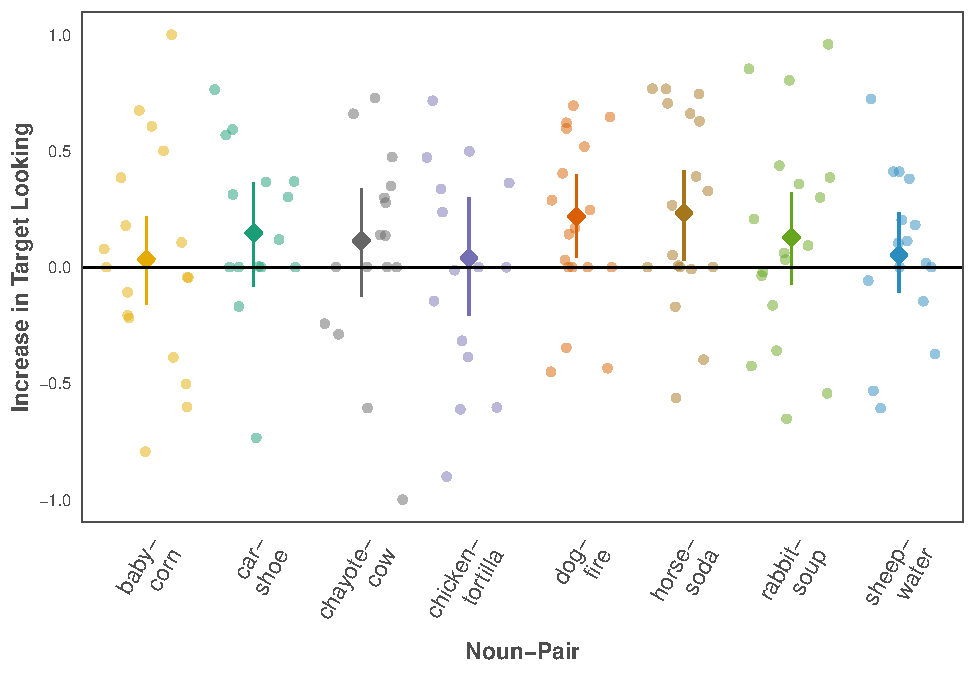
\includegraphics{revised_ms_analyses_files/figure-latex/r2-cn-by-item-plots-1.pdf}

\subsubsection{Scores By Subject}\label{scores-by-subject}

\begin{Shaded}
\begin{Highlighting}[]
\NormalTok{sub\_means\_tab }\OtherTok{\textless{}{-}}\NormalTok{ cn\_diffs\_df }\SpecialCharTok{\%\textgreater{}\%}
  \FunctionTok{filter}\NormalTok{(}\SpecialCharTok{!}\FunctionTok{is.na}\NormalTok{(noun\_pair\_diff)) }\SpecialCharTok{\%\textgreater{}\%}
  \FunctionTok{group\_by}\NormalTok{(subject\_id, bebe\_meses) }\SpecialCharTok{\%\textgreater{}\%}
  \FunctionTok{summarize}\NormalTok{(}\AttributeTok{n =} \FunctionTok{n}\NormalTok{(),}
    \AttributeTok{subj\_mean =} \FunctionTok{na.mean}\NormalTok{(noun\_pair\_diff))}

\NormalTok{positive\_scorers\_age\_tab }\OtherTok{\textless{}{-}}\NormalTok{ sub\_means\_tab }\SpecialCharTok{\%\textgreater{}\%}
  \FunctionTok{filter}\NormalTok{(subj\_mean}\SpecialCharTok{\textgreater{}}\DecValTok{0}\NormalTok{) }\SpecialCharTok{\%\textgreater{}\%}
  \FunctionTok{ungroup}\NormalTok{() }\SpecialCharTok{\%\textgreater{}\%}
  \FunctionTok{summarize}\NormalTok{(}\AttributeTok{min=}\FunctionTok{min}\NormalTok{(bebe\_meses),}
            \AttributeTok{max=}\FunctionTok{max}\NormalTok{(bebe\_meses),}
            \AttributeTok{mean=}\FunctionTok{mean}\NormalTok{(bebe\_meses),}
            \AttributeTok{sd=}\FunctionTok{sd}\NormalTok{(bebe\_meses),}
            \AttributeTok{ci.low=}\NormalTok{mean}\SpecialCharTok{{-}}\FunctionTok{ci.low}\NormalTok{(bebe\_meses),}
            \AttributeTok{ci.high=}\NormalTok{mean}\SpecialCharTok{+}\FunctionTok{ci.high}\NormalTok{(bebe\_meses))}

\NormalTok{N\_SUBS\_POSITIVE }\OtherTok{\textless{}{-}} \FunctionTok{sum}\NormalTok{(sub\_means\_tab}\SpecialCharTok{$}\NormalTok{subj\_mean}\SpecialCharTok{\textgreater{}}\DecValTok{0}\NormalTok{)}
\NormalTok{PS\_MIN\_AGE }\OtherTok{\textless{}{-}}\NormalTok{ positive\_scorers\_age\_tab}\SpecialCharTok{$}\NormalTok{min}
\NormalTok{PS\_MAX\_AGE }\OtherTok{\textless{}{-}}\NormalTok{ positive\_scorers\_age\_tab}\SpecialCharTok{$}\NormalTok{max}
\NormalTok{PS\_MEAN\_AGE }\OtherTok{\textless{}{-}}\NormalTok{ positive\_scorers\_age\_tab}\SpecialCharTok{$}\NormalTok{mean}
\NormalTok{PS\_CIL\_AGE }\OtherTok{\textless{}{-}}\NormalTok{ positive\_scorers\_age\_tab}\SpecialCharTok{$}\NormalTok{ci.low}
\NormalTok{PS\_CIH\_AGE }\OtherTok{\textless{}{-}}\NormalTok{ positive\_scorers\_age\_tab}\SpecialCharTok{$}\NormalTok{ci.high}
\NormalTok{PS\_SD\_AGE }\OtherTok{\textless{}{-}}\NormalTok{ positive\_scorers\_age\_tab}\SpecialCharTok{$}\NormalTok{sd}
\end{Highlighting}
\end{Shaded}

\begin{Shaded}
\begin{Highlighting}[]
\FunctionTok{set.seed}\NormalTok{(}\DecValTok{36}\NormalTok{)}

\NormalTok{ by\_sub\_overall\_tab }\OtherTok{\textless{}{-}}\NormalTok{ cn\_diffs\_df }\SpecialCharTok{\%\textgreater{}\%}
  \FunctionTok{group\_by}\NormalTok{(subject\_id) }\SpecialCharTok{\%\textgreater{}\%}
  \FunctionTok{summarize}\NormalTok{(}\AttributeTok{subj\_mean =} \FunctionTok{na.mean}\NormalTok{(noun\_pair\_diff)) }\SpecialCharTok{\%\textgreater{}\%}
  \FunctionTok{ungroup}\NormalTok{() }\SpecialCharTok{\%\textgreater{}\%}
  \FunctionTok{summarize}\NormalTok{(}\AttributeTok{group\_subject\_mean =} \FunctionTok{mean}\NormalTok{(subj\_mean),}
            \AttributeTok{min=}\FunctionTok{min}\NormalTok{(subj\_mean),}
            \AttributeTok{max=}\FunctionTok{max}\NormalTok{(subj\_mean),}
            \AttributeTok{ci.low=}\NormalTok{group\_subject\_mean}\SpecialCharTok{{-}}\FunctionTok{ci.low}\NormalTok{(subj\_mean),}
            \AttributeTok{ci.high =}\NormalTok{ group\_subject\_mean}\SpecialCharTok{+}\FunctionTok{ci.high}\NormalTok{(subj\_mean))}
 
\NormalTok{ALL\_SUB\_MEAN }\OtherTok{\textless{}{-}}\NormalTok{ by\_sub\_overall\_tab}\SpecialCharTok{$}\NormalTok{group\_subject\_mean}
\NormalTok{ALL\_SUB\_CIL }\OtherTok{\textless{}{-}}\NormalTok{ by\_sub\_overall\_tab}\SpecialCharTok{$}\NormalTok{ci.low}
\NormalTok{ALL\_SUB\_CIH }\OtherTok{\textless{}{-}}\NormalTok{ by\_sub\_overall\_tab}\SpecialCharTok{$}\NormalTok{ci.high}
\NormalTok{ALL\_SUB\_MIN }\OtherTok{\textless{}{-}}\NormalTok{ by\_sub\_overall\_tab}\SpecialCharTok{$}\NormalTok{min}
\NormalTok{ALL\_SUB\_MAX }\OtherTok{\textless{}{-}}\NormalTok{ by\_sub\_overall\_tab}\SpecialCharTok{$}\NormalTok{max}
\end{Highlighting}
\end{Shaded}

\paragraph{Non-parametric tests}\label{non-parametric-tests-1}

\begin{Shaded}
\begin{Highlighting}[]
\NormalTok{cn\_subj\_wilcox }\OtherTok{\textless{}{-}} \FunctionTok{wilcox.test}\NormalTok{(sub\_means\_tab}\SpecialCharTok{$}\NormalTok{subj\_mean, }\AttributeTok{mu=}\DecValTok{0}\NormalTok{, }
                              \AttributeTok{alternative=}\StringTok{\textquotesingle{}two.sided\textquotesingle{}}\NormalTok{)}

\NormalTok{CN\_SUBJ\_P\_WILCOX }\OtherTok{\textless{}{-}} \FunctionTok{reportP}\NormalTok{(cn\_subj\_wilcox}\SpecialCharTok{$}\NormalTok{p.value)}
\end{Highlighting}
\end{Shaded}

\begin{Shaded}
\begin{Highlighting}[]
\NormalTok{cn\_subj\_binom }\OtherTok{\textless{}{-}} \FunctionTok{binom.test}\NormalTok{(N\_SUBS\_POSITIVE, }\DecValTok{21}\NormalTok{, }\AttributeTok{p=}\NormalTok{.}\DecValTok{5}\NormalTok{)}

\NormalTok{CN\_SUBJ\_P\_BINOM }\OtherTok{\textless{}{-}} \FunctionTok{reportP}\NormalTok{(cn\_subj\_binom}\SpecialCharTok{$}\NormalTok{p.value)}
\end{Highlighting}
\end{Shaded}

\begin{Shaded}
\begin{Highlighting}[]
\FunctionTok{set.seed}\NormalTok{(}\DecValTok{36}\NormalTok{)}
\CommentTok{\# Bayes factor}
\FunctionTok{ttestBF}\NormalTok{(sub\_means\_tab}\SpecialCharTok{$}\NormalTok{subj\_mean)}
\end{Highlighting}
\end{Shaded}

\begin{verbatim}
## Bayes factor analysis
## --------------
## [1] Alt., r=0.707 : 5.8 ±0%
## 
## Against denominator:
##   Null, mu = 0 
## ---
## Bayes factor type: BFoneSample, JZS
\end{verbatim}

\begin{Shaded}
\begin{Highlighting}[]
\FunctionTok{ttestBF}\NormalTok{(sub\_means\_tab}\SpecialCharTok{$}\NormalTok{subj\_mean[sub\_means\_tab}\SpecialCharTok{$}\NormalTok{bebe\_meses}\SpecialCharTok{\textless{}}\DecValTok{10}\NormalTok{])}
\end{Highlighting}
\end{Shaded}

\begin{verbatim}
## Bayes factor analysis
## --------------
## [1] Alt., r=0.707 : 0.42 ±0.01%
## 
## Against denominator:
##   Null, mu = 0 
## ---
## Bayes factor type: BFoneSample, JZS
\end{verbatim}

\begin{Shaded}
\begin{Highlighting}[]
\FunctionTok{ttestBF}\NormalTok{(sub\_means\_tab}\SpecialCharTok{$}\NormalTok{subj\_mean[sub\_means\_tab}\SpecialCharTok{$}\NormalTok{bebe\_meses}\SpecialCharTok{\textgreater{}=}\DecValTok{10} \SpecialCharTok{\&} 
\NormalTok{                                  sub\_means\_tab}\SpecialCharTok{$}\NormalTok{bebe\_meses}\SpecialCharTok{\textless{}}\DecValTok{14}\NormalTok{])}
\end{Highlighting}
\end{Shaded}

\begin{verbatim}
## Bayes factor analysis
## --------------
## [1] Alt., r=0.707 : 2 ±0%
## 
## Against denominator:
##   Null, mu = 0 
## ---
## Bayes factor type: BFoneSample, JZS
\end{verbatim}

\begin{Shaded}
\begin{Highlighting}[]
\FunctionTok{ttestBF}\NormalTok{(sub\_means\_tab}\SpecialCharTok{$}\NormalTok{subj\_mean[sub\_means\_tab}\SpecialCharTok{$}\NormalTok{bebe\_meses}\SpecialCharTok{\textgreater{}=}\DecValTok{14}\NormalTok{])}
\end{Highlighting}
\end{Shaded}

\begin{verbatim}
## Bayes factor analysis
## --------------
## [1] Alt., r=0.707 : 1.1 ±0.04%
## 
## Against denominator:
##   Null, mu = 0 
## ---
## Bayes factor type: BFoneSample, JZS
\end{verbatim}

\begin{Shaded}
\begin{Highlighting}[]
\CommentTok{\# Standard deviation}
\NormalTok{stdev}\OtherTok{=}\FunctionTok{sd}\NormalTok{(sub\_means\_tab}\SpecialCharTok{$}\NormalTok{subj\_mean)}
\CommentTok{\# Mean}
\NormalTok{mean\_data}\OtherTok{=}\FunctionTok{mean}\NormalTok{(sub\_means\_tab}\SpecialCharTok{$}\NormalTok{subj\_mean)}
\CommentTok{\# Effect size}
\NormalTok{CN\_SUBJ\_D}\OtherTok{=}\FunctionTok{abs}\NormalTok{(mean\_data}\SpecialCharTok{/}\NormalTok{stdev)}
\end{Highlighting}
\end{Shaded}

\paragraph{MLM Intercept}\label{mlm-intercept}

\begin{Shaded}
\begin{Highlighting}[]
\FunctionTok{set.seed}\NormalTok{(}\DecValTok{36}\NormalTok{)}

\NormalTok{model0 }\OtherTok{\textless{}{-}} \FunctionTok{lmer}\NormalTok{(noun\_pair\_diff }\SpecialCharTok{\textasciitilde{}} \DecValTok{0} \SpecialCharTok{+}\NormalTok{ (}\DecValTok{1}\SpecialCharTok{|}\NormalTok{subject\_id), }\AttributeTok{REML =} \ConstantTok{FALSE}\NormalTok{,}
\NormalTok{             cn\_diffs\_df)}
\NormalTok{model1 }\OtherTok{\textless{}{-}} \FunctionTok{lmer}\NormalTok{(noun\_pair\_diff }\SpecialCharTok{\textasciitilde{}} \DecValTok{1} \SpecialCharTok{+}\NormalTok{ (}\DecValTok{1}\SpecialCharTok{|}\NormalTok{subject\_id), }\AttributeTok{REML =} \ConstantTok{FALSE}\NormalTok{,}
\NormalTok{               cn\_diffs\_df)}

\FunctionTok{xtable2kable}\NormalTok{(}\FunctionTok{summary}\NormalTok{(model1))}
\end{Highlighting}
\end{Shaded}

\begin{verbatim}
## Linear mixed model fit by maximum likelihood . t-tests use Satterthwaite's
##   method [lmerModLmerTest]
## Formula: noun_pair_diff ~ 1 + (1 | subject_id)
##    Data: cn_diffs_df
## 
##      AIC      BIC   logLik deviance df.resid 
##      176      185      -85      170      137 
## 
## Scaled residuals: 
##    Min     1Q Median     3Q    Max 
## -2.533 -0.435 -0.107  0.618  2.021 
## 
## Random effects:
##  Groups     Name        Variance Std.Dev.
##  subject_id (Intercept) 0.00301  0.0548  
##  Residual               0.19454  0.4411  
## Number of obs: 140, groups:  subject_id, 21
## 
## Fixed effects:
##             Estimate Std. Error      df t value Pr(>|t|)   
## (Intercept)   0.1218     0.0393 22.9081     3.1    0.005 **
## ---
## Signif. codes:  0 '***' 0.001 '**' 0.01 '*' 0.05 '.' 0.1 ' ' 1
\end{verbatim}

\begin{Shaded}
\begin{Highlighting}[]
\NormalTok{cn\_b0\_anova }\OtherTok{\textless{}{-}} \FunctionTok{anova}\NormalTok{(model1, model0)}
\NormalTok{CN\_B0\_CHISQ }\OtherTok{\textless{}{-}}\NormalTok{ cn\_b0\_anova}\SpecialCharTok{$}\NormalTok{Chisq[}\DecValTok{2}\NormalTok{]}
\NormalTok{CN\_B0\_CHI\_P }\OtherTok{\textless{}{-}} \FunctionTok{reportP}\NormalTok{(cn\_b0\_anova}\SpecialCharTok{$}\StringTok{\textasciigrave{}}\AttributeTok{Pr(\textgreater{}Chisq)}\StringTok{\textasciigrave{}}\NormalTok{[}\DecValTok{2}\NormalTok{])}

\NormalTok{all\_subs\_intercept }\OtherTok{\textless{}{-}} \FunctionTok{as.data.frame}\NormalTok{(}\FunctionTok{cbind}\NormalTok{(}\AttributeTok{b=}\FunctionTok{fixef}\NormalTok{(model1),}
                          \AttributeTok{ci.low=}\FunctionTok{confint}\NormalTok{(model1)[}\DecValTok{3}\NormalTok{,}\DecValTok{1}\NormalTok{], }
                          \AttributeTok{ci.high=}\FunctionTok{confint}\NormalTok{(model1)[}\DecValTok{3}\NormalTok{,}\DecValTok{2}\NormalTok{]))}

\NormalTok{CN\_B0\_EST }\OtherTok{\textless{}{-}}\NormalTok{ all\_subs\_intercept}\SpecialCharTok{$}\NormalTok{b}
\NormalTok{CN\_B0\_CIL }\OtherTok{\textless{}{-}}\NormalTok{ all\_subs\_intercept}\SpecialCharTok{$}\NormalTok{ci.low}
\NormalTok{CN\_B0\_CIH }\OtherTok{\textless{}{-}}\NormalTok{ all\_subs\_intercept}\SpecialCharTok{$}\NormalTok{ci.high}

\NormalTok{CN\_B0\_TT\_DF }\OtherTok{\textless{}{-}} \FunctionTok{as.numeric}\NormalTok{(}\FunctionTok{unlist}\NormalTok{(}\FunctionTok{summary}\NormalTok{(model1)[}\StringTok{\textquotesingle{}coefficients\textquotesingle{}}\NormalTok{])[}\DecValTok{3}\NormalTok{])}
\NormalTok{CN\_B0\_TT\_STAT }\OtherTok{\textless{}{-}} \FunctionTok{as.numeric}\NormalTok{(}\FunctionTok{unlist}\NormalTok{(}\FunctionTok{summary}\NormalTok{(model1)[}\StringTok{\textquotesingle{}coefficients\textquotesingle{}}\NormalTok{])[}\DecValTok{4}\NormalTok{])}
\NormalTok{CN\_B0\_TT\_P }\OtherTok{\textless{}{-}} \FunctionTok{reportP}\NormalTok{(}\FunctionTok{as.numeric}\NormalTok{(}\FunctionTok{unlist}\NormalTok{(}\FunctionTok{summary}\NormalTok{(model1)[}\StringTok{\textquotesingle{}coefficients\textquotesingle{}}\NormalTok{])[}\DecValTok{5}\NormalTok{]))}

\CommentTok{\#noun pair not enough variance to warrant random intercept}
\FunctionTok{write}\NormalTok{(}\FunctionTok{texreg}\NormalTok{(model1), }
      \AttributeTok{file=}\FunctionTok{here}\NormalTok{(}\StringTok{\textquotesingle{}supplement/tables/exp\_1/cn\_lmer0\_tab.tex\textquotesingle{}}\NormalTok{))}
\end{Highlighting}
\end{Shaded}

The mean of infants' subject-level scores was also positive (\textit{range:} \(-0.20-0.45\), \(M=0.11\) \textit{95\% CI:} {[}\(0.04\), \(0.18\){]}, \(p<.01\), Wilcoxon; \(p<.01\), \(\textit{Cohen's d}=0.64\)), with a majority (\(17/21\)) of infants (\(M_\textnormal{age}=11.19\)\textit{mos}, \({SD}_\textnormal{age}=2.74\)\textit{mos}) showing positive means across noun-pairs.

A linear mixed effects model with random intercepts for subjects indicates that these results were not driven by a few exceptional infants (\(\beta_0=0.12\), \textit{95\% CI:} {[}\(0.04\), \(0.20\){]},
\(t(22.91)=3.10\),
\(p<.01\); \(\chi^2(1)=7.89\), \(p<.01\); \(d=0.27\)).

\paragraph{Correlation with Age}\label{correlation-with-age}

\begin{Shaded}
\begin{Highlighting}[]
\FunctionTok{set.seed}\NormalTok{(}\DecValTok{36}\NormalTok{)}

\NormalTok{by\_subj\_age\_tab }\OtherTok{\textless{}{-}}\NormalTok{ cn\_diffs\_df }\SpecialCharTok{\%\textgreater{}\%} 
  \FunctionTok{group\_by}\NormalTok{(subject\_id, bebe\_meses, age\_centered) }\SpecialCharTok{\%\textgreater{}\%}
  \FunctionTok{summarize}\NormalTok{(}\AttributeTok{subj\_mean =} \FunctionTok{na.mean}\NormalTok{(noun\_pair\_diff),}
            \AttributeTok{n\_subjects =} \FunctionTok{n}\NormalTok{(),}
            \AttributeTok{min =} \FunctionTok{min}\NormalTok{(noun\_pair\_diff, }\AttributeTok{na.rm=}\NormalTok{T),}
            \AttributeTok{max =} \FunctionTok{max}\NormalTok{(noun\_pair\_diff, }\AttributeTok{na.rm=}\NormalTok{T),}
            \AttributeTok{ci.low =}\NormalTok{ subj\_mean}\SpecialCharTok{{-}}\FunctionTok{ci.low}\NormalTok{(noun\_pair\_diff),}
            \AttributeTok{ci.high =}\NormalTok{ subj\_mean}\SpecialCharTok{+}\FunctionTok{ci.high}\NormalTok{(noun\_pair\_diff)) }

\NormalTok{age\_cor\_test }\OtherTok{\textless{}{-}} \FunctionTok{cor.test}\NormalTok{(by\_subj\_age\_tab}\SpecialCharTok{$}\NormalTok{age\_centered, }
\NormalTok{                         by\_subj\_age\_tab}\SpecialCharTok{$}\NormalTok{subj\_mean,}
                         \AttributeTok{method=}\StringTok{\textquotesingle{}kendall\textquotesingle{}}\NormalTok{)}

\NormalTok{AGE\_CORR }\OtherTok{\textless{}{-}} \FunctionTok{as.numeric}\NormalTok{(age\_cor\_test}\SpecialCharTok{$}\NormalTok{estimate)}
\NormalTok{AGE\_CORR\_P }\OtherTok{\textless{}{-}} \FunctionTok{reportP}\NormalTok{(}\FunctionTok{as.numeric}\NormalTok{(age\_cor\_test}\SpecialCharTok{$}\NormalTok{p.value))}
\NormalTok{AGE\_CORR\_Z }\OtherTok{\textless{}{-}} \FunctionTok{as.numeric}\NormalTok{(age\_cor\_test}\SpecialCharTok{$}\NormalTok{statistic)}
\end{Highlighting}
\end{Shaded}

Subject-level scores exhibited an insignificant positive correlation with infants' age in months (\(\tau=0.25\), \(p=0.116\)).

\begin{Shaded}
\begin{Highlighting}[]
\FunctionTok{set.seed}\NormalTok{(}\DecValTok{36}\NormalTok{)}

\NormalTok{age\_cor\_test\_no15mo }\OtherTok{\textless{}{-}} \FunctionTok{cor.test}\NormalTok{(}
\NormalTok{  by\_subj\_age\_tab[by\_subj\_age\_tab}\SpecialCharTok{$}\NormalTok{bebe\_meses}\SpecialCharTok{\textless{}}\DecValTok{15}\NormalTok{,]}\SpecialCharTok{$}\NormalTok{bebe\_meses,}
\NormalTok{  by\_subj\_age\_tab[by\_subj\_age\_tab}\SpecialCharTok{$}\NormalTok{bebe\_meses}\SpecialCharTok{\textless{}}\DecValTok{15}\NormalTok{,]}\SpecialCharTok{$}\NormalTok{subj\_mean,}
  \AttributeTok{method=}\StringTok{\textquotesingle{}kendall\textquotesingle{}}\NormalTok{)}

\NormalTok{AGE\_OLDEST\_PP }\OtherTok{\textless{}{-}} \FunctionTok{max}\NormalTok{(by\_subj\_age\_tab}\SpecialCharTok{$}\NormalTok{bebe\_meses)}
\NormalTok{SCORE\_OLDEST\_PP }\OtherTok{\textless{}{-}} \FunctionTok{op}\NormalTok{(by\_subj\_age\_tab[}
\NormalTok{  by\_subj\_age\_tab}\SpecialCharTok{$}\NormalTok{bebe\_meses}\SpecialCharTok{==}\NormalTok{AGE\_OLDEST\_PP,]}\SpecialCharTok{$}\NormalTok{subj\_mean)}
\NormalTok{AGE\_CORR\_NO15MO }\OtherTok{\textless{}{-}} \FunctionTok{as.numeric}\NormalTok{(age\_cor\_test\_no15mo}\SpecialCharTok{$}\NormalTok{estimate)}
\NormalTok{AGE\_CORR\_P\_NO15MO }\OtherTok{\textless{}{-}} \FunctionTok{reportP}\NormalTok{(age\_cor\_test\_no15mo}\SpecialCharTok{$}\NormalTok{p.value)}
\NormalTok{AGE\_CORR\_Z\_NO15MO }\OtherTok{\textless{}{-}} \FunctionTok{as.numeric}\NormalTok{(age\_cor\_test\_no15mo}\SpecialCharTok{$}\NormalTok{statistic)}
\end{Highlighting}
\end{Shaded}

Excluding the one (oldest) participant (15.43 months) who showed notably low evidence of word recognition (\textit{mean difference score}\(=0.02\)), subject-level scores exhibited a significant (\(\alpha=0.05\)) positive correlation with infants' age in months (\(\tau=0.33\), \(p<.05\)).

\begin{Shaded}
\begin{Highlighting}[]
\NormalTok{age\_lm  }\OtherTok{\textless{}{-}} \FunctionTok{lm}\NormalTok{(subj\_mean }\SpecialCharTok{\textasciitilde{}} \DecValTok{1} \SpecialCharTok{+}\NormalTok{ age\_centered, by\_subj\_age\_tab)}
\FunctionTok{summary}\NormalTok{(age\_lm)}
\end{Highlighting}
\end{Shaded}

\begin{verbatim}
## 
## Call:
## lm(formula = subj_mean ~ 1 + age_centered, data = by_subj_age_tab)
## 
## Residuals:
##      Min       1Q   Median       3Q      Max 
## -0.24597 -0.14050  0.00887  0.09741  0.26630 
## 
## Coefficients:
##              Estimate Std. Error t value Pr(>|t|)   
## (Intercept)    0.1170     0.0372    3.15   0.0053 **
## age_centered   0.0226     0.0140    1.61   0.1241   
## ---
## Signif. codes:  0 '***' 0.001 '**' 0.01 '*' 0.05 '.' 0.1 ' ' 1
## 
## Residual standard error: 0.17 on 19 degrees of freedom
## Multiple R-squared:  0.12,   Adjusted R-squared:  0.0736 
## F-statistic: 2.59 on 1 and 19 DF,  p-value: 0.124
\end{verbatim}

\begin{Shaded}
\begin{Highlighting}[]
\FunctionTok{write}\NormalTok{(}\FunctionTok{texreg}\NormalTok{(age\_lm), }
      \AttributeTok{file=}\FunctionTok{here}\NormalTok{(}\StringTok{\textquotesingle{}supplement/tables/exp\_1/cn\_age\_lm\_tab.tex\textquotesingle{}}\NormalTok{)) }
\end{Highlighting}
\end{Shaded}

\subsubsection{Results Section text}\label{results-section-text}

All (\(8\)/8) noun-pairs showed positive mean scores, suggesting that the infants in our sample had knowledge of the nouns we tested, despite receiving very little directed speech (\(\textit{range:} 0.03-0.23\), \(M=0.12\), \textit{95\% bootstrapped CI:} {[}\(0.07\), \(0.17\){]}; \(p<.01\), Wilcoxon; \(p<.01\), binomial test; \(d=1.57\)).

The mean of infants' subject-level scores was also positive (\textit{range:} \(-0.20-0.45\), \(M=0.11\), \textit{95\% CI:} {[}\(0.04\), \(0.18\){]}; \(p<.01\), Wilcoxon; \(p<.01\), binomial; \(d=0.64\)), with a majority (\(17/21\)) of infants (\(M_\textnormal{age}=11.19\textit{mos}\), \({SD}_\textnormal{age}=2.74\textit{mos}\)) showing positive means across noun-pairs (see Figure in Supplement).

A linear mixed effects model with random intercepts for subjects\footnote{A model which additionally included random intercepts for item failed to converge.} indicates that these results were not driven by a few exceptional infants (\(\beta_0=0.12\), \textit{95\% CI:} {[}\(0.04\), \(0.20\){]},
\(t(22.91)=3.10\),
\(p<.01\); \(\chi^2(1)=7.89\), \(p<.01\); \(d=0.27\)).

\subsubsection{Comparison to B\&S 2012}\label{comparison-to-bs-2012}

\begin{Shaded}
\begin{Highlighting}[]
\NormalTok{cn\_diffs\_df }\SpecialCharTok{\%\textgreater{}\%} 
  \FunctionTok{filter}\NormalTok{(}\SpecialCharTok{!}\FunctionTok{is.na}\NormalTok{(noun\_pair\_diff)) }\SpecialCharTok{\%\textgreater{}\%}
  \FunctionTok{group\_by}\NormalTok{(subject\_id, bebe\_meses) }\SpecialCharTok{\%\textgreater{}\%}
  \FunctionTok{summarize}\NormalTok{(}\AttributeTok{subj\_mean =} \FunctionTok{na.mean}\NormalTok{(noun\_pair\_diff),}
            \AttributeTok{n\_items =} \FunctionTok{n}\NormalTok{()) }\SpecialCharTok{\%\textgreater{}\%}
  \FunctionTok{filter}\NormalTok{(}\SpecialCharTok{!}\FunctionTok{is.na}\NormalTok{(subj\_mean)) }\SpecialCharTok{\%\textgreater{}\%}
\FunctionTok{ggplot}\NormalTok{(.) }\SpecialCharTok{+}
  \FunctionTok{geom\_point}\NormalTok{(}\FunctionTok{aes}\NormalTok{(}\AttributeTok{x=}\NormalTok{bebe\_meses, }\AttributeTok{y=}\NormalTok{subj\_mean), }
             \AttributeTok{color=}\NormalTok{sheeppink, }\AttributeTok{alpha=}\NormalTok{.}\DecValTok{95}\NormalTok{, }\AttributeTok{shape=}\DecValTok{21}\NormalTok{, }\AttributeTok{size=}\FloatTok{2.5}\NormalTok{, }
             \AttributeTok{fill=}\NormalTok{sheeppink) }\SpecialCharTok{+} 
  \FunctionTok{geom\_linerange}\NormalTok{(}\FunctionTok{aes}\NormalTok{(}\AttributeTok{x=}\NormalTok{bebe\_meses, }
                     \AttributeTok{ymin=}\DecValTok{0}\NormalTok{, }\AttributeTok{ymax=}\NormalTok{subj\_mean), }
                 \AttributeTok{color=}\NormalTok{sheeppink) }\SpecialCharTok{+}
  \FunctionTok{geom\_hline}\NormalTok{(}\AttributeTok{yintercept=}\DecValTok{0}\NormalTok{) }\SpecialCharTok{+}
\NormalTok{  sb.density.theme }\SpecialCharTok{+}
  \FunctionTok{theme}\NormalTok{(}
    \AttributeTok{axis.title =} \FunctionTok{element\_text}\NormalTok{(}\AttributeTok{colour=}\StringTok{\textquotesingle{}gray30\textquotesingle{}}\NormalTok{, }\AttributeTok{size=}\DecValTok{11}\NormalTok{, }\AttributeTok{face=}\StringTok{\textquotesingle{}bold\textquotesingle{}}\NormalTok{),}
        \AttributeTok{axis.text =} \FunctionTok{element\_text}\NormalTok{(}\AttributeTok{colour=}\StringTok{\textquotesingle{}gray30\textquotesingle{}}\NormalTok{, }\AttributeTok{size=}\DecValTok{11}\NormalTok{),}
        \AttributeTok{axis.ticks =} \FunctionTok{element\_line}\NormalTok{(}\AttributeTok{colour=}\StringTok{\textquotesingle{}gray30\textquotesingle{}}\NormalTok{)) }\SpecialCharTok{+}
  \FunctionTok{ylab}\NormalTok{(}\StringTok{\textquotesingle{}Increase in Target Looking\textquotesingle{}}\NormalTok{) }\SpecialCharTok{+}
  \FunctionTok{xlab}\NormalTok{(}\StringTok{\textquotesingle{}Child Age (months)\textquotesingle{}}\NormalTok{) }\SpecialCharTok{+}
  \FunctionTok{xlim}\NormalTok{(}\FloatTok{4.5}\NormalTok{, }\FloatTok{16.0}\NormalTok{) }\SpecialCharTok{+}
  \FunctionTok{scale\_x\_continuous}\NormalTok{(}\AttributeTok{breaks=}\FunctionTok{c}\NormalTok{(}\DecValTok{4}\NormalTok{,}\DecValTok{5}\NormalTok{,}\DecValTok{6}\NormalTok{,}\DecValTok{7}\NormalTok{,}\DecValTok{8}\NormalTok{,}\DecValTok{9}\NormalTok{,}\DecValTok{10}\NormalTok{,}\DecValTok{11}\NormalTok{,}\DecValTok{12}\NormalTok{,}\DecValTok{13}\NormalTok{,}\DecValTok{14}\NormalTok{,}\DecValTok{15}\NormalTok{))}\SpecialCharTok{+}
  \FunctionTok{ylim}\NormalTok{(}\SpecialCharTok{{-}}\NormalTok{.}\DecValTok{4}\NormalTok{, .}\DecValTok{6}\NormalTok{) }
\end{Highlighting}
\end{Shaded}

\begin{figure}

{\centering 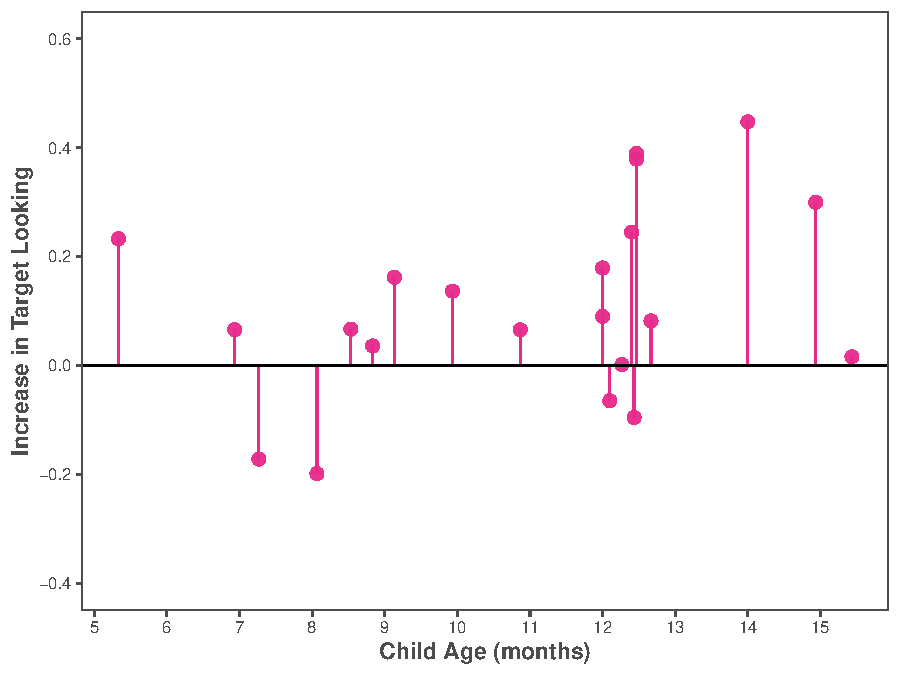
\includegraphics{revised_ms_analyses_files/figure-latex/r2-cn-by-subject-plot-incl-1} 

}

\caption{ }\label{fig:r2-cn-by-subject-plot-incl}
\end{figure}

\begin{Shaded}
\begin{Highlighting}[]
\FunctionTok{ggsave}\NormalTok{(}\FunctionTok{here}\NormalTok{(}\StringTok{\textquotesingle{}supplement/plots/exp\_1/pdfs\textquotesingle{}}\NormalTok{, }\StringTok{\textquotesingle{}cn\_meandiffs\_bysub.pdf\textquotesingle{}}\NormalTok{),}
       \AttributeTok{device=}\StringTok{\textquotesingle{}pdf\textquotesingle{}}\NormalTok{, }\AttributeTok{width=}\FloatTok{2.5}\NormalTok{, }\AttributeTok{height=}\FloatTok{1.5}\NormalTok{, }\AttributeTok{units=}\StringTok{\textquotesingle{}in\textquotesingle{}}\NormalTok{, }\AttributeTok{scale=}\DecValTok{2}\NormalTok{)}
\FunctionTok{ggsave}\NormalTok{(}\FunctionTok{here}\NormalTok{(}\StringTok{\textquotesingle{}supplement/plots/exp\_1/pngs\textquotesingle{}}\NormalTok{, }\StringTok{\textquotesingle{}cn\_meandiffs\_bysub.png\textquotesingle{}}\NormalTok{), }
       \AttributeTok{device=}\StringTok{\textquotesingle{}png\textquotesingle{}}\NormalTok{, }\AttributeTok{width=}\FloatTok{2.5}\NormalTok{, }\AttributeTok{height=}\FloatTok{1.5}\NormalTok{, }\AttributeTok{units=}\StringTok{\textquotesingle{}in\textquotesingle{}}\NormalTok{, }\AttributeTok{scale=}\DecValTok{2}\NormalTok{)}
\end{Highlighting}
\end{Shaded}

\begin{Shaded}
\begin{Highlighting}[]
\NormalTok{bysub\_agegroup\_means\_df }\OtherTok{\textless{}{-}} 
\NormalTok{  cn\_diffs\_df }\SpecialCharTok{\%\textgreater{}\%}
  \FunctionTok{group\_by}\NormalTok{(subject\_id, age\_group) }\SpecialCharTok{\%\textgreater{}\%}
  \FunctionTok{summarize}\NormalTok{(}\AttributeTok{subj\_mean =} \FunctionTok{na.mean}\NormalTok{(noun\_pair\_diff)) }\SpecialCharTok{\%\textgreater{}\%}
  \FunctionTok{group\_by}\NormalTok{(age\_group) }\SpecialCharTok{\%\textgreater{}\%}
  \FunctionTok{summarize}\NormalTok{(}\AttributeTok{age\_group\_M=}\FunctionTok{na.mean}\NormalTok{(subj\_mean))}

\NormalTok{CN\_SUBJ\_MDIFF\_6MOS }\OtherTok{\textless{}{-}} 
\NormalTok{  bysub\_agegroup\_means\_df}\SpecialCharTok{$}\NormalTok{age\_group\_M[}
\NormalTok{    bysub\_agegroup\_means\_df}\SpecialCharTok{$}\NormalTok{age\_group }\SpecialCharTok{==} \StringTok{\textquotesingle{}5{-}9 months\textquotesingle{}}\NormalTok{]}
\NormalTok{CN\_SUBJ\_MDIFF\_10MOS }\OtherTok{\textless{}{-}}
\NormalTok{  bysub\_agegroup\_means\_df}\SpecialCharTok{$}\NormalTok{age\_group\_M[}
\NormalTok{    bysub\_agegroup\_means\_df}\SpecialCharTok{$}\NormalTok{age\_group }\SpecialCharTok{==} \StringTok{\textquotesingle{}10{-}13 months\textquotesingle{}}\NormalTok{]}
\NormalTok{CN\_SUBJ\_MDIFF\_14MOS }\OtherTok{\textless{}{-}}
\NormalTok{  bysub\_agegroup\_means\_df}\SpecialCharTok{$}\NormalTok{age\_group\_M[}
\NormalTok{    bysub\_agegroup\_means\_df}\SpecialCharTok{$}\NormalTok{age\_group }\SpecialCharTok{==} \StringTok{\textquotesingle{}14{-}16 months\textquotesingle{}}\NormalTok{]}

\NormalTok{byitem\_agegroup\_means\_df }\OtherTok{\textless{}{-}}\NormalTok{ cn\_diffs\_df }\SpecialCharTok{\%\textgreater{}\%}
  \FunctionTok{filter}\NormalTok{(noun\_pair }\SpecialCharTok{\%in\%}\NormalTok{ noun\_pairs) }\SpecialCharTok{\%\textgreater{}\%}
  \FunctionTok{group\_by}\NormalTok{(age\_group, noun\_pair) }\SpecialCharTok{\%\textgreater{}\%}
  \FunctionTok{summarize}\NormalTok{(}\AttributeTok{item\_mean =} \FunctionTok{na.mean}\NormalTok{(noun\_pair\_diff)) }\SpecialCharTok{\%\textgreater{}\%}
  \FunctionTok{group\_by}\NormalTok{(age\_group) }\SpecialCharTok{\%\textgreater{}\%}
  \FunctionTok{summarize}\NormalTok{(}\AttributeTok{n =} \FunctionTok{n}\NormalTok{(),}
            \AttributeTok{age\_group\_M =} \FunctionTok{na.mean}\NormalTok{(item\_mean),}
            \AttributeTok{cil =}\NormalTok{ age\_group\_M }\SpecialCharTok{{-}} \FunctionTok{ci.low}\NormalTok{(item\_mean),}
            \AttributeTok{cih =}\NormalTok{ age\_group\_M }\SpecialCharTok{+} \FunctionTok{ci.high}\NormalTok{(item\_mean),}
            \AttributeTok{min =} \FunctionTok{min}\NormalTok{(item\_mean, }\AttributeTok{na.rm=}\NormalTok{T),}
            \AttributeTok{max =} \FunctionTok{max}\NormalTok{(item\_mean, }\AttributeTok{na.rm=}\NormalTok{T))}

\NormalTok{CN\_ITEM\_MDIFF\_6MOS }\OtherTok{\textless{}{-}} 
\NormalTok{  byitem\_agegroup\_means\_df}\SpecialCharTok{$}\NormalTok{age\_group\_M[}
\NormalTok{    byitem\_agegroup\_means\_df}\SpecialCharTok{$}\NormalTok{age\_group }\SpecialCharTok{==} \StringTok{\textquotesingle{}5{-}9 months\textquotesingle{}}\NormalTok{]}
\NormalTok{CN\_ITEM\_MDIFF\_10MOS }\OtherTok{\textless{}{-}} 
\NormalTok{  byitem\_agegroup\_means\_df}\SpecialCharTok{$}\NormalTok{age\_group\_M[}
\NormalTok{    byitem\_agegroup\_means\_df}\SpecialCharTok{$}\NormalTok{age\_group }\SpecialCharTok{==} \StringTok{\textquotesingle{}10{-}13 months\textquotesingle{}}\NormalTok{]}
\NormalTok{CN\_ITEM\_MDIFF\_14MOS }\OtherTok{\textless{}{-}} 
\NormalTok{  byitem\_agegroup\_means\_df}\SpecialCharTok{$}\NormalTok{age\_group\_M[}
\NormalTok{    byitem\_agegroup\_means\_df}\SpecialCharTok{$}\NormalTok{age\_group }\SpecialCharTok{==} \StringTok{\textquotesingle{}14{-}16 months\textquotesingle{}}\NormalTok{]}
\end{Highlighting}
\end{Shaded}

The evidence that Tseltal infants possessed knowledge of the words we probed is similarly strong to evidence that has been used to infer the presence of word knowledge among U.S. infants. For example, Bergelson and Swingley (2012) reported mean scores of 0.074 (over subjects) and 0.065 (over items) for 6- to 9-month--olds, 0.055 (over subjects) and 0.059 (over items) for 10- to 13-month--olds, and 0.29 (over subjects) and 0.28 (over items) for 14-16--month-olds.

We found: mean scores of 0.04 (over subjects) and 0.03 (over items) for 6- to 9-month--olds, 0.13 (over subjects) and 0.12 (over items) for 10- to 13-month--olds, and 0.25 (over subjects) and 0.26 (over items) for 14- to 16-month--olds.

\section{EXCLUSION CRITERIA 2 (EC2)}\label{exclusion-criteria-2-ec2}

\subsection{Replicating Mean Difference Analysis (EC2)}\label{replicating-mean-difference-analysis-ec2}

\emph{Including only infants affording calculation of at least half (4) of \textbf{difference scores} (rather than contributing half of all trials)}

\emph{Under this criterion, total sample includes:}

\begin{verbatim}
_- 8 infants with calculable difference scores for all 8 noun-pairs_  
_- 7 infants with calculable difference scores for 7/8_    
_- 2 infants with calculable scores for 6/8_  
_- 1 infant with a calculable score for 5/8_    
_- 2 infants with calculable scores for 4/8_    
\end{verbatim}

\emph{- 1 EXCLUDED participant with calculable scores for only 2/8 (fewer than half of the set of noun-pairs).}

\emph{N=20}

\subsubsection{Scores By Item (EC2)}\label{scores-by-item-ec2}

\begin{Shaded}
\begin{Highlighting}[]
\FunctionTok{set.seed}\NormalTok{(}\DecValTok{36}\NormalTok{)}

\NormalTok{by\_item\_tab2 }\OtherTok{\textless{}{-}}\NormalTok{ cn\_diffs\_df }\SpecialCharTok{\%\textgreater{}\%} 
  \FunctionTok{filter}\NormalTok{(subject\_id}\SpecialCharTok{!=}\StringTok{\textquotesingle{}J94252\textquotesingle{}}\NormalTok{) }\SpecialCharTok{\%\textgreater{}\%}
  \FunctionTok{group\_by}\NormalTok{(noun\_pair, subject\_id) }\SpecialCharTok{\%\textgreater{}\%}
  \FunctionTok{summarize}\NormalTok{(}\AttributeTok{subj\_mean =} \FunctionTok{na.mean}\NormalTok{(noun\_pair\_diff)) }\SpecialCharTok{\%\textgreater{}\%}
  \FunctionTok{ungroup}\NormalTok{() }\SpecialCharTok{\%\textgreater{}\%}
  \FunctionTok{group\_by}\NormalTok{(noun\_pair) }\SpecialCharTok{\%\textgreater{}\%}
  \FunctionTok{summarize}\NormalTok{(}\AttributeTok{n\_subjects =} \FunctionTok{n}\NormalTok{(),}
            \AttributeTok{item\_mean =} \FunctionTok{na.mean}\NormalTok{(subj\_mean),}
            \AttributeTok{median =} \FunctionTok{median}\NormalTok{(subj\_mean, }\AttributeTok{na.rm=}\NormalTok{T),}
            \AttributeTok{ci.low=}\NormalTok{item\_mean}\SpecialCharTok{{-}}\FunctionTok{ci.low}\NormalTok{(subj\_mean),}
            \AttributeTok{ci.high =}\NormalTok{ item\_mean}\SpecialCharTok{+}\FunctionTok{ci.high}\NormalTok{(subj\_mean),}
            \AttributeTok{min=}\FunctionTok{min}\NormalTok{(subj\_mean, }\AttributeTok{na.rm=}\NormalTok{T),}
            \AttributeTok{max=}\FunctionTok{max}\NormalTok{(subj\_mean, }\AttributeTok{na.rm=}\NormalTok{T)) }

\NormalTok{ALL\_ITEM\_MEAN2 }\OtherTok{\textless{}{-}} \FunctionTok{mean}\NormalTok{(by\_item\_tab2}\SpecialCharTok{$}\NormalTok{item\_mean)}
\NormalTok{ALL\_ITEM\_CIL2 }\OtherTok{\textless{}{-}}\NormalTok{ ALL\_ITEM\_MEAN }\SpecialCharTok{{-}} \FunctionTok{ci.low}\NormalTok{(by\_item\_tab2}\SpecialCharTok{$}\NormalTok{item\_mean)}
\NormalTok{ALL\_ITEM\_CIH2 }\OtherTok{\textless{}{-}}\NormalTok{ ALL\_ITEM\_MEAN }\SpecialCharTok{+} \FunctionTok{ci.high}\NormalTok{(by\_item\_tab2}\SpecialCharTok{$}\NormalTok{item\_mean)}
\NormalTok{ALL\_ITEM\_MIN2 }\OtherTok{\textless{}{-}} \FunctionTok{min}\NormalTok{(by\_item\_tab2}\SpecialCharTok{$}\NormalTok{item\_mean)}
\NormalTok{ALL\_ITEM\_MAX2 }\OtherTok{\textless{}{-}} \FunctionTok{max}\NormalTok{(by\_item\_tab2}\SpecialCharTok{$}\NormalTok{item\_mean)}
\NormalTok{N\_ITEMS\_POSITIVE2 }\OtherTok{\textless{}{-}} \FunctionTok{sum}\NormalTok{(by\_item\_tab2}\SpecialCharTok{$}\NormalTok{item\_mean}\SpecialCharTok{\textgreater{}}\DecValTok{0}\NormalTok{)}
\end{Highlighting}
\end{Shaded}

\begin{Shaded}
\begin{Highlighting}[]
\FunctionTok{set.seed}\NormalTok{(}\DecValTok{36}\NormalTok{)}

\NormalTok{by\_item\_tab2 }\OtherTok{\textless{}{-}}\NormalTok{ cn\_diffs\_df }\SpecialCharTok{\%\textgreater{}\%}
  \FunctionTok{filter}\NormalTok{(subject\_id}\SpecialCharTok{!=}\StringTok{\textquotesingle{}J94252\textquotesingle{}}\NormalTok{) }\SpecialCharTok{\%\textgreater{}\%}
  \FunctionTok{group\_by}\NormalTok{(noun\_pair, subject\_id) }\SpecialCharTok{\%\textgreater{}\%}
  \FunctionTok{summarize}\NormalTok{(}\AttributeTok{subj\_mean =} \FunctionTok{na.mean}\NormalTok{(noun\_pair\_diff)) }\SpecialCharTok{\%\textgreater{}\%}
  \FunctionTok{ungroup}\NormalTok{() }\SpecialCharTok{\%\textgreater{}\%}
  \FunctionTok{group\_by}\NormalTok{(noun\_pair) }\SpecialCharTok{\%\textgreater{}\%}
  \FunctionTok{summarize}\NormalTok{(}\AttributeTok{n =} \FunctionTok{n}\NormalTok{(),}
            \AttributeTok{M =} \FunctionTok{na.mean}\NormalTok{(subj\_mean),}
            \AttributeTok{cil=}\NormalTok{M}\SpecialCharTok{{-}}\FunctionTok{ci.low}\NormalTok{(subj\_mean),}
            \AttributeTok{cih =}\NormalTok{ M}\SpecialCharTok{+}\FunctionTok{ci.high}\NormalTok{(subj\_mean),}
            \AttributeTok{min=}\FunctionTok{min}\NormalTok{(subj\_mean, }\AttributeTok{na.rm=}\NormalTok{T),}
            \AttributeTok{max=}\FunctionTok{max}\NormalTok{(subj\_mean, }\AttributeTok{na.rm=}\NormalTok{T))}

\FunctionTok{xtable2kable}\NormalTok{(by\_item\_tab2)}
\end{Highlighting}
\end{Shaded}

\begin{verbatim}
## # A tibble: 8 x 7
##   noun_pair            n      M     cil   cih    min   max
##   <chr>            <int>  <dbl>   <dbl> <dbl>  <dbl> <dbl>
## 1 baby-corn           20 0.0359 -0.183  0.251 -0.794 1    
## 2 car-shoe            18 0.146  -0.0860 0.359 -1     1    
## 3 chayote-cow         18 0.113  -0.108  0.335 -1     1    
## 4 chicken-tortilla    20 0.0401 -0.205  0.291 -0.901 1    
## 5 dog-fire            20 0.217   0.0374 0.394 -0.450 1    
## 6 horse-soda          20 0.269   0.0896 0.437 -0.563 0.768
## 7 rabbit-soup         20 0.127  -0.0850 0.348 -0.653 0.959
## 8 sheep-water         20 0.0517 -0.111  0.214 -0.606 0.723
\end{verbatim}

\paragraph{Non-parametric Tests (EC2)}\label{non-parametric-tests-ec2}

\begin{Shaded}
\begin{Highlighting}[]
\NormalTok{cn\_item\_wilcox2 }\OtherTok{\textless{}{-}} \FunctionTok{wilcox.test}\NormalTok{(by\_item\_tab2}\SpecialCharTok{$}\NormalTok{M, }\AttributeTok{mu=}\DecValTok{0}\NormalTok{,}
                              \AttributeTok{alternative=}\StringTok{\textquotesingle{}two.sided\textquotesingle{}}\NormalTok{)}

\NormalTok{CN\_ITEM\_P\_WILCOX2 }\OtherTok{\textless{}{-}} \FunctionTok{reportP}\NormalTok{(cn\_item\_wilcox2}\SpecialCharTok{$}\NormalTok{p.value)}
\end{Highlighting}
\end{Shaded}

\begin{Shaded}
\begin{Highlighting}[]
\NormalTok{cn\_item\_binom2 }\OtherTok{\textless{}{-}} \FunctionTok{binom.test}\NormalTok{(N\_ITEMS\_POSITIVE2, }\DecValTok{8}\NormalTok{, }\AttributeTok{p=}\NormalTok{.}\DecValTok{5}\NormalTok{)}

\NormalTok{CN\_ITEM\_P\_BINOM2 }\OtherTok{\textless{}{-}} \FunctionTok{reportP}\NormalTok{(cn\_item\_binom2}\SpecialCharTok{$}\NormalTok{p.value)}
\end{Highlighting}
\end{Shaded}

\begin{Shaded}
\begin{Highlighting}[]
\FunctionTok{set.seed}\NormalTok{(}\DecValTok{36}\NormalTok{)}
\CommentTok{\# Bayes factor}
\FunctionTok{ttestBF}\NormalTok{(by\_item\_tab2}\SpecialCharTok{$}\NormalTok{M)}
\end{Highlighting}
\end{Shaded}

\begin{verbatim}
## Bayes factor analysis
## --------------
## [1] Alt., r=0.707 : 13 ±0%
## 
## Against denominator:
##   Null, mu = 0 
## ---
## Bayes factor type: BFoneSample, JZS
\end{verbatim}

\begin{Shaded}
\begin{Highlighting}[]
\CommentTok{\# Standard deviation}
\NormalTok{stdev}\OtherTok{=}\FunctionTok{sd}\NormalTok{(by\_item\_tab2}\SpecialCharTok{$}\NormalTok{M)}
\CommentTok{\# Mean}
\NormalTok{mean\_data}\OtherTok{=}\FunctionTok{mean}\NormalTok{(by\_item\_tab2}\SpecialCharTok{$}\NormalTok{M)}
\CommentTok{\# Effect size}
\NormalTok{CN\_ITEM\_D2}\OtherTok{=}\FunctionTok{abs}\NormalTok{(mean\_data}\SpecialCharTok{/}\NormalTok{stdev)}
\end{Highlighting}
\end{Shaded}

When implementing this new, even more stringent exclusion criteria (leading us to drop an entire participant's data), \(8\)/8 noun-pairs showed a positive mean difference score (\(0.04-0.27\), \(M=0.12\) \textit{95\% CI:} {[}\(0.06\), \(0.17\){]}; \(p<.01\), Wilcoxon test; \(p<.01\), binomial test, \(d=1.47\)).

\subsubsection{Scores By Subject (EC2)}\label{scores-by-subject-ec2}

\begin{Shaded}
\begin{Highlighting}[]
\NormalTok{sub\_means\_tab2 }\OtherTok{\textless{}{-}}\NormalTok{ cn\_diffs\_df }\SpecialCharTok{\%\textgreater{}\%}
  \FunctionTok{filter}\NormalTok{(}\SpecialCharTok{!}\FunctionTok{is.na}\NormalTok{(noun\_pair\_diff), }
\NormalTok{         subject\_id }\SpecialCharTok{!=} \StringTok{\textquotesingle{}J94252\textquotesingle{}}\NormalTok{) }\SpecialCharTok{\%\textgreater{}\%}
  \FunctionTok{group\_by}\NormalTok{(subject\_id, bebe\_meses) }\SpecialCharTok{\%\textgreater{}\%}
  \FunctionTok{summarize}\NormalTok{(}\AttributeTok{n =} \FunctionTok{n}\NormalTok{(),}
    \AttributeTok{subj\_mean =} \FunctionTok{na.mean}\NormalTok{(noun\_pair\_diff))}

\NormalTok{positive\_scorers\_age\_tab2 }\OtherTok{\textless{}{-}}\NormalTok{ sub\_means\_tab2 }\SpecialCharTok{\%\textgreater{}\%}
  \FunctionTok{filter}\NormalTok{(subj\_mean}\SpecialCharTok{\textgreater{}}\DecValTok{0}\NormalTok{) }\SpecialCharTok{\%\textgreater{}\%}
  \FunctionTok{ungroup}\NormalTok{() }\SpecialCharTok{\%\textgreater{}\%}
  \FunctionTok{summarize}\NormalTok{(}\AttributeTok{min=}\FunctionTok{min}\NormalTok{(bebe\_meses),}
            \AttributeTok{max=}\FunctionTok{max}\NormalTok{(bebe\_meses),}
            \AttributeTok{mean=}\FunctionTok{mean}\NormalTok{(bebe\_meses),}
            \AttributeTok{sd=}\FunctionTok{sd}\NormalTok{(bebe\_meses),}
            \AttributeTok{ci.low=}\NormalTok{mean}\SpecialCharTok{{-}}\FunctionTok{ci.low}\NormalTok{(bebe\_meses),}
            \AttributeTok{ci.high=}\NormalTok{mean}\SpecialCharTok{+}\FunctionTok{ci.high}\NormalTok{(bebe\_meses))}

\NormalTok{N2 }\OtherTok{\textless{}{-}} \FunctionTok{length}\NormalTok{(}\FunctionTok{unique}\NormalTok{(sub\_means\_tab2}\SpecialCharTok{$}\NormalTok{subject\_id))}

\NormalTok{N\_SUBS\_POSITIVE2 }\OtherTok{\textless{}{-}} \FunctionTok{sum}\NormalTok{(sub\_means\_tab2}\SpecialCharTok{$}\NormalTok{subj\_mean}\SpecialCharTok{\textgreater{}}\DecValTok{0}\NormalTok{)}
\NormalTok{PS\_MIN\_AGE2 }\OtherTok{\textless{}{-}}\NormalTok{ positive\_scorers\_age\_tab2}\SpecialCharTok{$}\NormalTok{min}
\NormalTok{PS\_MAX\_AGE2 }\OtherTok{\textless{}{-}}\NormalTok{ positive\_scorers\_age\_tab2}\SpecialCharTok{$}\NormalTok{max}
\NormalTok{PS\_MEAN\_AGE2 }\OtherTok{\textless{}{-}}\NormalTok{ positive\_scorers\_age\_tab2}\SpecialCharTok{$}\NormalTok{mean}
\NormalTok{PS\_CIL\_AGE2 }\OtherTok{\textless{}{-}}\NormalTok{ positive\_scorers\_age\_tab2}\SpecialCharTok{$}\NormalTok{ci.low}
\NormalTok{PS\_CIH\_AGE2 }\OtherTok{\textless{}{-}}\NormalTok{ positive\_scorers\_age\_tab2}\SpecialCharTok{$}\NormalTok{ci.high}
\NormalTok{PS\_SD\_AGE2 }\OtherTok{\textless{}{-}}\NormalTok{ positive\_scorers\_age\_tab2}\SpecialCharTok{$}\NormalTok{sd}
\end{Highlighting}
\end{Shaded}

\(17/20\) subjects showed a positive mean difference score (\textit{range}: \(-10.10\)\textit{yrs}, \(M_{age}=11.19\) \textit{95\% CI:} {[}\(9.90\), \(12.33\){]}, \(SD_{age}=2.74\)).

\begin{Shaded}
\begin{Highlighting}[]
\FunctionTok{set.seed}\NormalTok{(}\DecValTok{36}\NormalTok{)}

\NormalTok{ by\_sub\_overall\_tab2 }\OtherTok{\textless{}{-}}\NormalTok{ cn\_diffs\_df }\SpecialCharTok{\%\textgreater{}\%}
  \FunctionTok{filter}\NormalTok{(subject\_id }\SpecialCharTok{!=} \StringTok{\textquotesingle{}J94252\textquotesingle{}}\NormalTok{) }\SpecialCharTok{\%\textgreater{}\%}
  \FunctionTok{group\_by}\NormalTok{(subject\_id) }\SpecialCharTok{\%\textgreater{}\%}
  \FunctionTok{summarize}\NormalTok{(}\AttributeTok{subj\_mean =} \FunctionTok{na.mean}\NormalTok{(noun\_pair\_diff)) }\SpecialCharTok{\%\textgreater{}\%}
  \FunctionTok{ungroup}\NormalTok{() }\SpecialCharTok{\%\textgreater{}\%}
  \FunctionTok{summarize}\NormalTok{(}\AttributeTok{group\_subject\_mean =} \FunctionTok{mean}\NormalTok{(subj\_mean),}
            \AttributeTok{min=}\FunctionTok{min}\NormalTok{(subj\_mean),}
            \AttributeTok{max=}\FunctionTok{max}\NormalTok{(subj\_mean),}
            \AttributeTok{ci.low=}\NormalTok{group\_subject\_mean}\SpecialCharTok{{-}}\FunctionTok{ci.low}\NormalTok{(subj\_mean),}
            \AttributeTok{ci.high =}\NormalTok{ group\_subject\_mean}\SpecialCharTok{+}\FunctionTok{ci.high}\NormalTok{(subj\_mean))}
 
\NormalTok{ALL\_SUB\_MEAN2 }\OtherTok{\textless{}{-}}\NormalTok{ by\_sub\_overall\_tab2}\SpecialCharTok{$}\NormalTok{group\_subject\_mean}
\NormalTok{ALL\_SUB\_CIL2 }\OtherTok{\textless{}{-}}\NormalTok{ by\_sub\_overall\_tab2}\SpecialCharTok{$}\NormalTok{ci.low}
\NormalTok{ALL\_SUB\_CIH2 }\OtherTok{\textless{}{-}}\NormalTok{ by\_sub\_overall\_tab2}\SpecialCharTok{$}\NormalTok{ci.high}
\NormalTok{ALL\_SUB\_MIN2 }\OtherTok{\textless{}{-}}\NormalTok{ by\_sub\_overall\_tab2}\SpecialCharTok{$}\NormalTok{min}
\NormalTok{ALL\_SUB\_MAX2 }\OtherTok{\textless{}{-}}\NormalTok{ by\_sub\_overall\_tab2}\SpecialCharTok{$}\NormalTok{max}
\end{Highlighting}
\end{Shaded}

\paragraph{MLM Intercept (EC2)}\label{mlm-intercept-ec2}

\begin{Shaded}
\begin{Highlighting}[]
\FunctionTok{set.seed}\NormalTok{(}\DecValTok{36}\NormalTok{)}

\CommentTok{\#noun pair not enough variance to warrant random intercept}
\NormalTok{model0\_2 }\OtherTok{\textless{}{-}} \FunctionTok{lmer}\NormalTok{(noun\_pair\_diff }\SpecialCharTok{\textasciitilde{}} \DecValTok{0} \SpecialCharTok{+}\NormalTok{ (}\DecValTok{1}\SpecialCharTok{|}\NormalTok{subject\_id), }\AttributeTok{REML =} \ConstantTok{FALSE}\NormalTok{,}
\NormalTok{             cn\_diffs\_df[cn\_diffs\_df}\SpecialCharTok{$}\NormalTok{subject\_id}\SpecialCharTok{!=}\StringTok{\textquotesingle{}J94252\textquotesingle{}}\NormalTok{,])}
\NormalTok{model1\_2 }\OtherTok{\textless{}{-}} \FunctionTok{lmer}\NormalTok{(noun\_pair\_diff }\SpecialCharTok{\textasciitilde{}} \DecValTok{1} \SpecialCharTok{+}\NormalTok{ (}\DecValTok{1}\SpecialCharTok{|}\NormalTok{subject\_id), }\AttributeTok{REML =} \ConstantTok{FALSE}\NormalTok{,}
\NormalTok{               cn\_diffs\_df[cn\_diffs\_df}\SpecialCharTok{$}\NormalTok{subject\_id}\SpecialCharTok{!=}\StringTok{\textquotesingle{}J94252\textquotesingle{}}\NormalTok{,])}

\FunctionTok{xtable2kable}\NormalTok{(}\FunctionTok{summary}\NormalTok{(model1\_2))}
\end{Highlighting}
\end{Shaded}

\begin{verbatim}
## Linear mixed model fit by maximum likelihood . t-tests use Satterthwaite's
##   method [lmerModLmerTest]
## Formula: noun_pair_diff ~ 1 + (1 | subject_id)
##    Data: cn_diffs_df[cn_diffs_df$subject_id != "J94252", ]
## 
##      AIC      BIC   logLik deviance df.resid 
##      174      183      -84      168      135 
## 
## Scaled residuals: 
##     Min      1Q  Median      3Q     Max 
## -2.5378 -0.4097 -0.0874  0.6331  2.0047 
## 
## Random effects:
##  Groups     Name        Variance Std.Dev.
##  subject_id (Intercept) 0.00287  0.0535  
##  Residual               0.19546  0.4421  
## Number of obs: 138, groups:  subject_id, 20
## 
## Fixed effects:
##             Estimate Std. Error      df t value Pr(>|t|)   
## (Intercept)   0.1269     0.0395 22.3564    3.21    0.004 **
## ---
## Signif. codes:  0 '***' 0.001 '**' 0.01 '*' 0.05 '.' 0.1 ' ' 1
\end{verbatim}

\begin{Shaded}
\begin{Highlighting}[]
\NormalTok{cn\_b0\_anova\_2 }\OtherTok{\textless{}{-}} \FunctionTok{anova}\NormalTok{(model1\_2, model0\_2)}
\NormalTok{CN\_B0\_CHISQ2 }\OtherTok{\textless{}{-}}\NormalTok{ cn\_b0\_anova\_2}\SpecialCharTok{$}\NormalTok{Chisq[}\DecValTok{2}\NormalTok{]}
\NormalTok{CN\_B0\_CHI\_P2 }\OtherTok{\textless{}{-}} \FunctionTok{reportP}\NormalTok{(cn\_b0\_anova\_2}\SpecialCharTok{$}\StringTok{\textasciigrave{}}\AttributeTok{Pr(\textgreater{}Chisq)}\StringTok{\textasciigrave{}}\NormalTok{[}\DecValTok{2}\NormalTok{])}

\NormalTok{all\_subs\_intercept2 }\OtherTok{\textless{}{-}} \FunctionTok{as.data.frame}\NormalTok{(}\FunctionTok{cbind}\NormalTok{(}\AttributeTok{b=}\FunctionTok{fixef}\NormalTok{(model1\_2),}
                          \AttributeTok{ci.low=}\FunctionTok{confint}\NormalTok{(model1\_2)[}\DecValTok{3}\NormalTok{,}\DecValTok{1}\NormalTok{], }
                          \AttributeTok{ci.high=}\FunctionTok{confint}\NormalTok{(model1\_2)[}\DecValTok{3}\NormalTok{,}\DecValTok{2}\NormalTok{]))}

\NormalTok{CN\_B0\_EST2 }\OtherTok{\textless{}{-}}\NormalTok{ all\_subs\_intercept2}\SpecialCharTok{$}\NormalTok{b}
\NormalTok{CN\_B0\_CIL2 }\OtherTok{\textless{}{-}}\NormalTok{ all\_subs\_intercept2}\SpecialCharTok{$}\NormalTok{ci.low}
\NormalTok{CN\_B0\_CIH2 }\OtherTok{\textless{}{-}}\NormalTok{ all\_subs\_intercept2}\SpecialCharTok{$}\NormalTok{ci.high}

\NormalTok{CN\_B0\_TT\_DF2 }\OtherTok{\textless{}{-}} \FunctionTok{as.numeric}\NormalTok{(}\FunctionTok{unlist}\NormalTok{(}\FunctionTok{summary}\NormalTok{(model1\_2)[}\StringTok{\textquotesingle{}coefficients\textquotesingle{}}\NormalTok{])[}\DecValTok{3}\NormalTok{])}
\NormalTok{CN\_B0\_TT\_STAT2 }\OtherTok{\textless{}{-}} \FunctionTok{as.numeric}\NormalTok{(}\FunctionTok{unlist}\NormalTok{(}\FunctionTok{summary}\NormalTok{(model1\_2)[}\StringTok{\textquotesingle{}coefficients\textquotesingle{}}\NormalTok{])[}\DecValTok{4}\NormalTok{])}
\NormalTok{CN\_B0\_TT\_P2 }\OtherTok{\textless{}{-}} \FunctionTok{reportP}\NormalTok{(}\FunctionTok{as.numeric}\NormalTok{(}\FunctionTok{unlist}\NormalTok{(}\FunctionTok{summary}\NormalTok{(model1\_2)[}\StringTok{\textquotesingle{}coefficients\textquotesingle{}}\NormalTok{])[}\DecValTok{5}\NormalTok{]))}
\end{Highlighting}
\end{Shaded}

\paragraph{Non-parametric tests (EC2)}\label{non-parametric-tests-ec2-1}

\begin{Shaded}
\begin{Highlighting}[]
\NormalTok{cn\_subj\_wilcox2 }\OtherTok{\textless{}{-}} \FunctionTok{wilcox.test}\NormalTok{(sub\_means\_tab2}\SpecialCharTok{$}\NormalTok{subj\_mean, }\AttributeTok{mu=}\DecValTok{0}\NormalTok{, }
                              \AttributeTok{alternative=}\StringTok{\textquotesingle{}two.sided\textquotesingle{}}\NormalTok{)}

\NormalTok{CN\_SUBJ\_P\_WILCOX2 }\OtherTok{\textless{}{-}} \FunctionTok{reportP}\NormalTok{(cn\_subj\_wilcox2}\SpecialCharTok{$}\NormalTok{p.value)}
\end{Highlighting}
\end{Shaded}

\begin{Shaded}
\begin{Highlighting}[]
\NormalTok{cn\_subj\_binom2 }\OtherTok{\textless{}{-}} \FunctionTok{binom.test}\NormalTok{(N\_SUBS\_POSITIVE2, N2, }\AttributeTok{p=}\FloatTok{0.5}\NormalTok{)}

\NormalTok{CN\_SUBJ\_P\_BINOM2 }\OtherTok{\textless{}{-}} \FunctionTok{reportP}\NormalTok{(cn\_subj\_binom2}\SpecialCharTok{$}\NormalTok{p.value)}
\end{Highlighting}
\end{Shaded}

\begin{Shaded}
\begin{Highlighting}[]
\FunctionTok{set.seed}\NormalTok{(}\DecValTok{36}\NormalTok{)}
\CommentTok{\# Bayes factor}
\FunctionTok{ttestBF}\NormalTok{(sub\_means\_tab2}\SpecialCharTok{$}\NormalTok{subj\_mean)}
\end{Highlighting}
\end{Shaded}

\begin{verbatim}
## Bayes factor analysis
## --------------
## [1] Alt., r=0.707 : 16 ±0%
## 
## Against denominator:
##   Null, mu = 0 
## ---
## Bayes factor type: BFoneSample, JZS
\end{verbatim}

\begin{Shaded}
\begin{Highlighting}[]
\CommentTok{\# Standard deviation}
\NormalTok{stdev}\OtherTok{=}\FunctionTok{sd}\NormalTok{(sub\_means\_tab2}\SpecialCharTok{$}\NormalTok{subj\_mean)}
\CommentTok{\# Mean}
\NormalTok{mean\_data}\OtherTok{=}\FunctionTok{mean}\NormalTok{(sub\_means\_tab2}\SpecialCharTok{$}\NormalTok{subj\_mean)}
\CommentTok{\# Effect size}
\NormalTok{CN\_SUBJ\_D2}\OtherTok{=}\FunctionTok{abs}\NormalTok{(mean\_data}\SpecialCharTok{/}\NormalTok{stdev)}
\end{Highlighting}
\end{Shaded}

Using this alternative interpretation of the reviewer's suggested exclusion criteria, the mean across all \(20\) subjects was positive (\textit{range:} \(-0.17-0.45\), \(M=0.13\) \textit{95\% CI:} {[}\(0.06\), \(0.20\){]}; \(p<.01\), Wilcoxon; \(p<.01\), binomial, \(d=0.77\)).

A linear mixed effects model with random intercepts for subjects suggests that these results were reliable across infants (\(\beta_0=0.13\), \textit{95\% CI:} {[}\(0.05\), \(0.21\){]}, \(t(22.36)=3.21\),
\(p<.01\); \(\chi^2(1)=8.45\), \(p<.01\); \(d=0.28\)).

\paragraph{Replicating Correlation with Age (EC2)}\label{replicating-correlation-with-age-ec2}

\begin{Shaded}
\begin{Highlighting}[]
\FunctionTok{set.seed}\NormalTok{(}\DecValTok{36}\NormalTok{)}

\NormalTok{by\_subj\_age\_tab2 }\OtherTok{\textless{}{-}}\NormalTok{ cn\_diffs\_df }\SpecialCharTok{\%\textgreater{}\%} 
  \FunctionTok{filter}\NormalTok{(subject\_id }\SpecialCharTok{!=} \StringTok{\textquotesingle{}J94252\textquotesingle{}}\NormalTok{) }\SpecialCharTok{\%\textgreater{}\%}
  \FunctionTok{group\_by}\NormalTok{(subject\_id, bebe\_meses, age\_centered) }\SpecialCharTok{\%\textgreater{}\%}
  \FunctionTok{summarize}\NormalTok{(}\AttributeTok{subj\_mean =} \FunctionTok{na.mean}\NormalTok{(noun\_pair\_diff),}
            \AttributeTok{n\_subjects =} \FunctionTok{n}\NormalTok{(),}
            \AttributeTok{min =} \FunctionTok{min}\NormalTok{(noun\_pair\_diff, }\AttributeTok{na.rm=}\NormalTok{T),}
            \AttributeTok{max =} \FunctionTok{max}\NormalTok{(noun\_pair\_diff, }\AttributeTok{na.rm=}\NormalTok{T),}
            \AttributeTok{ci.low =}\NormalTok{ subj\_mean}\SpecialCharTok{{-}}\FunctionTok{ci.low}\NormalTok{(noun\_pair\_diff),}
            \AttributeTok{ci.high =}\NormalTok{ subj\_mean}\SpecialCharTok{+}\FunctionTok{ci.high}\NormalTok{(noun\_pair\_diff)) }

\NormalTok{age\_cor\_test2 }\OtherTok{\textless{}{-}} \FunctionTok{cor.test}\NormalTok{(by\_subj\_age\_tab2}\SpecialCharTok{$}\NormalTok{age\_centered, }
\NormalTok{                         by\_subj\_age\_tab2}\SpecialCharTok{$}\NormalTok{subj\_mean,}
                         \AttributeTok{method=}\StringTok{\textquotesingle{}kendall\textquotesingle{}}\NormalTok{)}

\NormalTok{AGE\_CORR2 }\OtherTok{\textless{}{-}} \FunctionTok{as.numeric}\NormalTok{(age\_cor\_test2}\SpecialCharTok{$}\NormalTok{estimate)}
\NormalTok{AGE\_CORR\_P2 }\OtherTok{\textless{}{-}} \FunctionTok{as.numeric}\NormalTok{(age\_cor\_test2}\SpecialCharTok{$}\NormalTok{p.value)}
\NormalTok{AGE\_CORR\_Z2 }\OtherTok{\textless{}{-}} \FunctionTok{as.numeric}\NormalTok{(age\_cor\_test2}\SpecialCharTok{$}\NormalTok{statistic)}
\end{Highlighting}
\end{Shaded}

Using this alternate exclusion criteria, children's age in months exhibited an insignificant positive correlation with their mean difference scores across items (\(\tau=0.20\), \(p=0.22\)).

\begin{Shaded}
\begin{Highlighting}[]
\NormalTok{age\_lm2  }\OtherTok{\textless{}{-}} \FunctionTok{lm}\NormalTok{(subj\_mean }\SpecialCharTok{\textasciitilde{}} \DecValTok{1} \SpecialCharTok{+}\NormalTok{ age\_centered, by\_subj\_age\_tab2)}
\FunctionTok{summary}\NormalTok{(age\_lm2)}
\end{Highlighting}
\end{Shaded}

\begin{verbatim}
## 
## Call:
## lm(formula = subj_mean ~ 1 + age_centered, data = by_subj_age_tab2)
## 
## Residuals:
##      Min       1Q   Median       3Q      Max 
## -0.24652 -0.09133 -0.00413  0.09738  0.26970 
## 
## Coefficients:
##              Estimate Std. Error t value Pr(>|t|)   
## (Intercept)    0.1290     0.0365    3.53   0.0024 **
## age_centered   0.0171     0.0139    1.23   0.2335   
## ---
## Signif. codes:  0 '***' 0.001 '**' 0.01 '*' 0.05 '.' 0.1 ' ' 1
## 
## Residual standard error: 0.16 on 18 degrees of freedom
## Multiple R-squared:  0.0779, Adjusted R-squared:  0.0266 
## F-statistic: 1.52 on 1 and 18 DF,  p-value: 0.234
\end{verbatim}

\section{Pre/Post Looking Logit Model}\label{prepost-looking-logit-model}

\emph{Dueling exclusion criteria are not relevant here, as even participant `J94252' contributed at least half (16) of all test trials.}

\begin{Shaded}
\begin{Highlighting}[]
\NormalTok{cn\_supp\_pre }\OtherTok{\textless{}{-}}\NormalTok{ cn\_fin }\SpecialCharTok{\%\textgreater{}\%}
  \FunctionTok{select}\NormalTok{(pre\_target\_sum\_ms, pre\_nontarget\_sum\_ms, }
\NormalTok{         subject\_id, bebe\_meses, age\_centered, noun\_pair)  }

\NormalTok{cn\_supp\_pre}\SpecialCharTok{$}\NormalTok{phase }\OtherTok{\textless{}{-}} \StringTok{\textquotesingle{}pre{-}naming\textquotesingle{}}
\NormalTok{cn\_supp\_pre}\SpecialCharTok{$}\NormalTok{target\_bins }\OtherTok{\textless{}{-}} \FunctionTok{round}\NormalTok{(cn\_supp\_pre}\SpecialCharTok{$}\NormalTok{pre\_target\_sum\_ms}\SpecialCharTok{/}\DecValTok{20}\NormalTok{,}\DecValTok{0}\NormalTok{)}
\NormalTok{cn\_supp\_pre}\SpecialCharTok{$}\NormalTok{nontarget\_bins }\OtherTok{\textless{}{-}} \FunctionTok{round}\NormalTok{(cn\_supp\_pre}\SpecialCharTok{$}\NormalTok{pre\_nontarget\_sum\_ms}\SpecialCharTok{/}\DecValTok{20}\NormalTok{, }\DecValTok{0}\NormalTok{)}

\NormalTok{cn\_supp\_pre }\OtherTok{\textless{}{-}}\NormalTok{ cn\_supp\_pre }\SpecialCharTok{\%\textgreater{}\%} 
  \FunctionTok{select}\NormalTok{(subject\_id, bebe\_meses, age\_centered, }
\NormalTok{         noun\_pair, phase, target\_bins, nontarget\_bins) }

\NormalTok{cn\_supp\_post }\OtherTok{\textless{}{-}}\NormalTok{ cn\_fin }\SpecialCharTok{\%\textgreater{}\%}
  \FunctionTok{select}\NormalTok{(post1\_target\_sum\_ms, post1\_nontarget\_sum\_ms, }
\NormalTok{         subject\_id, bebe\_meses, age\_centered, noun\_pair)}

\NormalTok{cn\_supp\_post}\SpecialCharTok{$}\NormalTok{phase }\OtherTok{\textless{}{-}} \StringTok{\textquotesingle{}post{-}naming\textquotesingle{}}
\NormalTok{cn\_supp\_post}\SpecialCharTok{$}\NormalTok{target\_bins }\OtherTok{\textless{}{-}} \FunctionTok{round}\NormalTok{(cn\_supp\_post}\SpecialCharTok{$}\NormalTok{post1\_target\_sum\_ms}\SpecialCharTok{/}\DecValTok{20}\NormalTok{,}\DecValTok{0}\NormalTok{)}
\NormalTok{cn\_supp\_post}\SpecialCharTok{$}\NormalTok{nontarget\_bins }\OtherTok{\textless{}{-}} \FunctionTok{round}\NormalTok{(cn\_supp\_post}\SpecialCharTok{$}\NormalTok{post1\_nontarget\_sum\_ms}\SpecialCharTok{/}\DecValTok{20}\NormalTok{,}\DecValTok{0}\NormalTok{)}

\NormalTok{cn\_supp\_post }\OtherTok{\textless{}{-}}\NormalTok{ cn\_supp\_post }\SpecialCharTok{\%\textgreater{}\%} 
  \FunctionTok{select}\NormalTok{(subject\_id, bebe\_meses, age\_centered, }
\NormalTok{         noun\_pair, phase, target\_bins, nontarget\_bins) }

\NormalTok{cn\_supp\_stacked\_r2 }\OtherTok{\textless{}{-}} \FunctionTok{rbind}\NormalTok{(cn\_supp\_pre, cn\_supp\_post)}

\NormalTok{cn\_supp\_stacked\_r2}\SpecialCharTok{$}\NormalTok{phase }\OtherTok{\textless{}{-}} \FunctionTok{as.factor}\NormalTok{(cn\_supp\_stacked\_r2}\SpecialCharTok{$}\NormalTok{phase)}
\NormalTok{cn\_supp\_stacked\_r2}\SpecialCharTok{$}\NormalTok{phase }\OtherTok{\textless{}{-}} \FunctionTok{relevel}\NormalTok{(cn\_supp\_stacked\_r2}\SpecialCharTok{$}\NormalTok{phase, }\AttributeTok{ref=}\StringTok{\textquotesingle{}pre{-}naming\textquotesingle{}}\NormalTok{)}

\NormalTok{cn\_supp\_stacked\_r2 }\SpecialCharTok{\%\textgreater{}\%}
  \FunctionTok{group\_by}\NormalTok{(subject\_id, bebe\_meses, age\_centered, noun\_pair, phase) }\SpecialCharTok{\%\textgreater{}\%}
  \FunctionTok{reframe}\NormalTok{(}\AttributeTok{target\_bins =}\NormalTok{ target\_bins, }
            \AttributeTok{nontarget\_bins =}\NormalTok{ nontarget\_bins) }\SpecialCharTok{\%\textgreater{}\%}
\FunctionTok{write.csv}\NormalTok{(., }\FunctionTok{here}\NormalTok{(}\StringTok{\textquotesingle{}data/r\_analysis\_dfs\textquotesingle{}}\NormalTok{, }
                  \StringTok{\textquotesingle{}cn\_prepost\_target\_looking.csv\textquotesingle{}}\NormalTok{)}
\NormalTok{          )}
\end{Highlighting}
\end{Shaded}

\begin{Shaded}
\begin{Highlighting}[]
\FunctionTok{set.seed}\NormalTok{(}\DecValTok{36}\NormalTok{)}
\NormalTok{cn\_supp\_glmer\_null }\OtherTok{\textless{}{-}} \FunctionTok{glmer}\NormalTok{(}\FunctionTok{cbind}\NormalTok{(target\_bins, nontarget\_bins) }\SpecialCharTok{\textasciitilde{}}
                         \DecValTok{1} \SpecialCharTok{+}\NormalTok{ (}\DecValTok{1}\SpecialCharTok{|}\NormalTok{subject\_id) }\SpecialCharTok{+}\NormalTok{ (}\DecValTok{1}\SpecialCharTok{|}\NormalTok{noun\_pair),}
                        \AttributeTok{family=}\NormalTok{binomial, cn\_supp\_stacked\_r2)}

\NormalTok{cn\_supp\_glmer }\OtherTok{\textless{}{-}} \FunctionTok{glmer}\NormalTok{(}\FunctionTok{cbind}\NormalTok{(target\_bins, nontarget\_bins) }\SpecialCharTok{\textasciitilde{}}
\NormalTok{                         phase }\SpecialCharTok{+}\NormalTok{ (}\DecValTok{1}\SpecialCharTok{|}\NormalTok{subject\_id) }\SpecialCharTok{+}\NormalTok{ (}\DecValTok{1}\SpecialCharTok{|}\NormalTok{noun\_pair),}
                        \AttributeTok{family=}\NormalTok{binomial, cn\_supp\_stacked\_r2)}

\FunctionTok{summary}\NormalTok{(cn\_supp\_glmer)}
\end{Highlighting}
\end{Shaded}

\begin{verbatim}
## Generalized linear mixed model fit by maximum likelihood (Laplace
##   Approximation) [glmerMod]
##  Family: binomial  ( logit )
## Formula: cbind(target_bins, nontarget_bins) ~ phase + (1 | subject_id) +  
##     (1 | noun_pair)
##    Data: cn_supp_stacked_r2
## 
##      AIC      BIC   logLik deviance df.resid 
##   114954   114973   -57473   114946     1052 
## 
## Scaled residuals: 
##     Min      1Q  Median      3Q     Max 
## -20.196  -7.622   0.822   7.850  19.954 
## 
## Random effects:
##  Groups     Name        Variance Std.Dev.
##  subject_id (Intercept) 0.0327   0.181   
##  noun_pair  (Intercept) 0.0234   0.153   
## Number of obs: 1056, groups:  subject_id, 21; noun_pair, 8
## 
## Fixed effects:
##                  Estimate Std. Error z value Pr(>|z|)    
## (Intercept)       0.02640    0.06726    0.39     0.69    
## phasepost-naming  0.24900    0.00983   25.32   <2e-16 ***
## ---
## Signif. codes:  0 '***' 0.001 '**' 0.01 '*' 0.05 '.' 0.1 ' ' 1
## 
## Correlation of Fixed Effects:
##             (Intr)
## phspst-nmng -0.059
\end{verbatim}

\begin{Shaded}
\begin{Highlighting}[]
\NormalTok{cn\_supp\_glmer\_tab }\OtherTok{\textless{}{-}} \FunctionTok{as.data.frame}\NormalTok{(}
  \FunctionTok{cbind}\NormalTok{(}\StringTok{\textquotesingle{}OR\textquotesingle{}}\OtherTok{=}\FunctionTok{op}\NormalTok{(}\FunctionTok{exp}\NormalTok{(}\FunctionTok{fixef}\NormalTok{(cn\_supp\_glmer))),}
        \StringTok{\textquotesingle{}CIL\textquotesingle{}}\OtherTok{=}\FunctionTok{op}\NormalTok{(}\FunctionTok{exp}\NormalTok{(}\FunctionTok{confint}\NormalTok{(cn\_supp\_glmer))[}\DecValTok{3}\SpecialCharTok{:}\DecValTok{4}\NormalTok{,}\DecValTok{1}\NormalTok{]),}
        \StringTok{\textquotesingle{}CIH\textquotesingle{}}\OtherTok{=}\FunctionTok{op}\NormalTok{(}\FunctionTok{exp}\NormalTok{(}\FunctionTok{confint}\NormalTok{(cn\_supp\_glmer))[}\DecValTok{3}\SpecialCharTok{:}\DecValTok{4}\NormalTok{,}\DecValTok{2}\NormalTok{])))}

\NormalTok{POSTNAMING\_OR }\OtherTok{\textless{}{-}}\NormalTok{ cn\_supp\_glmer\_tab}\SpecialCharTok{$}\NormalTok{OR[}\DecValTok{2}\NormalTok{]}
\NormalTok{POSTNAMING\_CIL }\OtherTok{\textless{}{-}}\NormalTok{ cn\_supp\_glmer\_tab}\SpecialCharTok{$}\NormalTok{CIL[}\DecValTok{2}\NormalTok{]}
\NormalTok{POSTNAMING\_CIH }\OtherTok{\textless{}{-}}\NormalTok{ cn\_supp\_glmer\_tab}\SpecialCharTok{$}\NormalTok{CIH[}\DecValTok{2}\NormalTok{]}
\NormalTok{PHASE\_WALD\_CHISQ }\OtherTok{\textless{}{-}} \FunctionTok{Anova}\NormalTok{(cn\_supp\_glmer)[}\StringTok{\textquotesingle{}phase\textquotesingle{}}\NormalTok{,}\StringTok{\textquotesingle{}Chisq\textquotesingle{}}\NormalTok{]}
\NormalTok{PHASE\_WALD\_P }\OtherTok{\textless{}{-}} \FunctionTok{reportP}\NormalTok{(}\FunctionTok{Anova}\NormalTok{(cn\_supp\_glmer)[}\StringTok{\textquotesingle{}phase\textquotesingle{}}\NormalTok{,}\StringTok{\textquotesingle{}Pr(\textgreater{}Chisq)\textquotesingle{}}\NormalTok{])}

\FunctionTok{anova}\NormalTok{(cn\_supp\_glmer\_null, cn\_supp\_glmer)}
\end{Highlighting}
\end{Shaded}

\begin{verbatim}
## Data: cn_supp_stacked_r2
## Models:
## cn_supp_glmer_null: cbind(target_bins, nontarget_bins) ~ 1 + (1 | subject_id) + (1 | noun_pair)
## cn_supp_glmer: cbind(target_bins, nontarget_bins) ~ phase + (1 | subject_id) + (1 | noun_pair)
##                    npar    AIC    BIC logLik deviance Chisq Df Pr(>Chisq)    
## cn_supp_glmer_null    3 115594 115609 -57794   115588                        
## cn_supp_glmer         4 114953 114973 -57473   114945   643  1     <2e-16 ***
## ---
## Signif. codes:  0 '***' 0.001 '**' 0.01 '*' 0.05 '.' 0.1 ' ' 1
\end{verbatim}

\begin{Shaded}
\begin{Highlighting}[]
\FunctionTok{Anova}\NormalTok{(cn\_supp\_glmer)}
\end{Highlighting}
\end{Shaded}

\begin{verbatim}
## Analysis of Deviance Table (Type II Wald chisquare tests)
## 
## Response: cbind(target_bins, nontarget_bins)
##       Chisq Df Pr(>Chisq)    
## phase   641  1     <2e-16 ***
## ---
## Signif. codes:  0 '***' 0.001 '**' 0.01 '*' 0.05 '.' 0.1 ' ' 1
\end{verbatim}

Model summary shows that model is fit on 1056 observations from 21 subjects
(number of trials = 1056/2 = 528, as model is fit to data in `long' form,
where two rows for each trial: pre-naming and post-naming).

\begin{Shaded}
\begin{Highlighting}[]
\NormalTok{cn\_supp\_stacked\_r2}\SpecialCharTok{$}\NormalTok{ratio }\OtherTok{\textless{}{-}}\NormalTok{ cn\_supp\_stacked\_r2}\SpecialCharTok{$}\NormalTok{target\_bins}\SpecialCharTok{/}
\NormalTok{  cn\_supp\_stacked\_r2}\SpecialCharTok{$}\NormalTok{nontarget\_bins}

\NormalTok{cn\_supp\_age\_glmer }\OtherTok{\textless{}{-}} \FunctionTok{glmer}\NormalTok{(}\FunctionTok{cbind}\NormalTok{(target\_bins, nontarget\_bins) }\SpecialCharTok{\textasciitilde{}}
\NormalTok{                         phase }\SpecialCharTok{+}\NormalTok{ age\_centered }\SpecialCharTok{+} 
\NormalTok{                           (}\DecValTok{1}\SpecialCharTok{|}\NormalTok{subject\_id) }\SpecialCharTok{+}\NormalTok{ (}\DecValTok{1}\SpecialCharTok{|}\NormalTok{noun\_pair),}
                        \AttributeTok{family=}\NormalTok{binomial, cn\_supp\_stacked\_r2)}

\NormalTok{cn\_pp\_age\_glmer\_tab }\OtherTok{\textless{}{-}} \FunctionTok{as.data.frame}\NormalTok{(}
  \FunctionTok{cbind}\NormalTok{(}\StringTok{\textquotesingle{}OR\textquotesingle{}}\OtherTok{=}\FunctionTok{op}\NormalTok{(}\FunctionTok{exp}\NormalTok{(}\FunctionTok{fixef}\NormalTok{(cn\_supp\_age\_glmer))),}
        \StringTok{\textquotesingle{}CIL\textquotesingle{}}\OtherTok{=}\FunctionTok{op}\NormalTok{(}\FunctionTok{exp}\NormalTok{(}\FunctionTok{confint}\NormalTok{(cn\_supp\_age\_glmer))[}\DecValTok{3}\SpecialCharTok{:}\DecValTok{5}\NormalTok{,}\DecValTok{1}\NormalTok{]),}
        \StringTok{\textquotesingle{}CIH\textquotesingle{}}\OtherTok{=}\FunctionTok{op}\NormalTok{(}\FunctionTok{exp}\NormalTok{(}\FunctionTok{confint}\NormalTok{(cn\_supp\_age\_glmer))[}\DecValTok{3}\SpecialCharTok{:}\DecValTok{5}\NormalTok{,}\DecValTok{2}\NormalTok{])))}

\FunctionTok{anova}\NormalTok{(cn\_supp\_glmer, cn\_supp\_age\_glmer)}
\end{Highlighting}
\end{Shaded}

\begin{verbatim}
## Data: cn_supp_stacked_r2
## Models:
## cn_supp_glmer: cbind(target_bins, nontarget_bins) ~ phase + (1 | subject_id) + (1 | noun_pair)
## cn_supp_age_glmer: cbind(target_bins, nontarget_bins) ~ phase + age_centered + (1 | subject_id) + (1 | noun_pair)
##                   npar    AIC    BIC logLik deviance Chisq Df Pr(>Chisq)
## cn_supp_glmer        4 114953 114973 -57473   114945                    
## cn_supp_age_glmer    5 114955 114980 -57473   114945   0.1  1       0.75
\end{verbatim}

\begin{Shaded}
\begin{Highlighting}[]
\FunctionTok{Anova}\NormalTok{(cn\_supp\_age\_glmer)}
\end{Highlighting}
\end{Shaded}

\begin{verbatim}
## Analysis of Deviance Table (Type II Wald chisquare tests)
## 
## Response: cbind(target_bins, nontarget_bins)
##              Chisq Df Pr(>Chisq)    
## phase        641.1  1     <2e-16 ***
## age_centered   0.1  1       0.75    
## ---
## Signif. codes:  0 '***' 0.001 '**' 0.01 '*' 0.05 '.' 0.1 ' ' 1
\end{verbatim}

\begin{Shaded}
\begin{Highlighting}[]
\NormalTok{cn\_supp\_ageint\_glmer }\OtherTok{\textless{}{-}} \FunctionTok{glmer}\NormalTok{(}\FunctionTok{cbind}\NormalTok{(target\_bins, nontarget\_bins) }\SpecialCharTok{\textasciitilde{}}
\NormalTok{                         phase}\SpecialCharTok{*}\NormalTok{age\_centered }\SpecialCharTok{+} 
\NormalTok{                           (}\DecValTok{1}\SpecialCharTok{|}\NormalTok{subject\_id) }\SpecialCharTok{+}\NormalTok{ (}\DecValTok{1}\SpecialCharTok{|}\NormalTok{noun\_pair),}
                        \AttributeTok{family=}\NormalTok{binomial, cn\_supp\_stacked\_r2)}

\NormalTok{cn\_supp\_ageint\_glmer\_tab }\OtherTok{\textless{}{-}} \FunctionTok{as.data.frame}\NormalTok{(}
  \FunctionTok{cbind}\NormalTok{(}\StringTok{\textquotesingle{}OR\textquotesingle{}}\OtherTok{=}\FunctionTok{op}\NormalTok{(}\FunctionTok{exp}\NormalTok{(}\FunctionTok{fixef}\NormalTok{(cn\_supp\_ageint\_glmer))),}
        \StringTok{\textquotesingle{}CIL\textquotesingle{}}\OtherTok{=}\FunctionTok{op}\NormalTok{(}\FunctionTok{exp}\NormalTok{(}\FunctionTok{confint}\NormalTok{(cn\_supp\_ageint\_glmer))[}\DecValTok{3}\SpecialCharTok{:}\DecValTok{6}\NormalTok{,}\DecValTok{1}\NormalTok{]),}
        \StringTok{\textquotesingle{}CIH\textquotesingle{}}\OtherTok{=}\FunctionTok{op}\NormalTok{(}\FunctionTok{exp}\NormalTok{(}\FunctionTok{confint}\NormalTok{(cn\_supp\_ageint\_glmer))[}\DecValTok{3}\SpecialCharTok{:}\DecValTok{6}\NormalTok{,}\DecValTok{2}\NormalTok{])))}

\DocumentationTok{\#\# reporting effect of trial phase}
\NormalTok{POST\_AGE\_INT\_PHASE\_OR }\OtherTok{\textless{}{-}}\NormalTok{ cn\_supp\_ageint\_glmer\_tab}\SpecialCharTok{$}\NormalTok{OR[}\DecValTok{2}\NormalTok{]}
\NormalTok{POST\_AGE\_INT\_PHASE\_CIL }\OtherTok{\textless{}{-}}\NormalTok{ cn\_supp\_ageint\_glmer\_tab}\SpecialCharTok{$}\NormalTok{CIL[}\DecValTok{2}\NormalTok{]}
\NormalTok{POST\_AGE\_INT\_PHASE\_CIH }\OtherTok{\textless{}{-}}\NormalTok{ cn\_supp\_ageint\_glmer\_tab}\SpecialCharTok{$}\NormalTok{CIH[}\DecValTok{2}\NormalTok{]}
\NormalTok{POST\_AGE\_INT\_PHASE\_WALD\_CHISQ }\OtherTok{\textless{}{-}} 
  \FunctionTok{Anova}\NormalTok{(cn\_supp\_ageint\_glmer)[}\StringTok{\textquotesingle{}phase\textquotesingle{}}\NormalTok{,}\StringTok{\textquotesingle{}Chisq\textquotesingle{}}\NormalTok{]}
\NormalTok{POST\_AGE\_INT\_PHASE\_WALD\_P }\OtherTok{\textless{}{-}}
  \FunctionTok{reportP}\NormalTok{(}\FunctionTok{Anova}\NormalTok{(cn\_supp\_ageint\_glmer)[}\StringTok{\textquotesingle{}phase\textquotesingle{}}\NormalTok{,}\StringTok{\textquotesingle{}Pr(\textgreater{}Chisq)\textquotesingle{}}\NormalTok{])}

\DocumentationTok{\#\# reporting interaction between phase and age}
\NormalTok{POST\_AGE\_INT\_OR }\OtherTok{\textless{}{-}}\NormalTok{ cn\_supp\_ageint\_glmer\_tab}\SpecialCharTok{$}\NormalTok{OR[}\DecValTok{4}\NormalTok{]}
\NormalTok{POST\_AGE\_INT\_CIL }\OtherTok{\textless{}{-}}\NormalTok{ cn\_supp\_ageint\_glmer\_tab}\SpecialCharTok{$}\NormalTok{CIL[}\DecValTok{4}\NormalTok{]}
\NormalTok{POST\_AGE\_INT\_CIH }\OtherTok{\textless{}{-}}\NormalTok{ cn\_supp\_ageint\_glmer\_tab}\SpecialCharTok{$}\NormalTok{CIH[}\DecValTok{4}\NormalTok{]}
\NormalTok{POST\_AGE\_INT\_WALD\_CHISQ }\OtherTok{\textless{}{-}} 
  \FunctionTok{Anova}\NormalTok{(cn\_supp\_ageint\_glmer)[}\StringTok{\textquotesingle{}phase:age\_centered\textquotesingle{}}\NormalTok{,}\StringTok{\textquotesingle{}Chisq\textquotesingle{}}\NormalTok{]}
\NormalTok{POST\_AGE\_INT\_WALD\_P }\OtherTok{\textless{}{-}}
  \FunctionTok{reportP}\NormalTok{(}\FunctionTok{Anova}\NormalTok{(cn\_supp\_ageint\_glmer)[}\StringTok{\textquotesingle{}phase:age\_centered\textquotesingle{}}\NormalTok{,}\StringTok{\textquotesingle{}Pr(\textgreater{}Chisq)\textquotesingle{}}\NormalTok{])}

\DocumentationTok{\#\# comparing interaction model to model with phase alone}
\NormalTok{cn\_supp\_ageint\_anova }\OtherTok{\textless{}{-}} \FunctionTok{anova}\NormalTok{(cn\_supp\_glmer, cn\_supp\_ageint\_glmer)}

\NormalTok{POST\_AGE\_INT\_DF }\OtherTok{\textless{}{-}}\NormalTok{ cn\_supp\_ageint\_anova}\SpecialCharTok{$}\NormalTok{Df[}\DecValTok{2}\NormalTok{]}
\NormalTok{POST\_AGE\_INT\_CHISQ }\OtherTok{\textless{}{-}}\NormalTok{ cn\_supp\_ageint\_anova}\SpecialCharTok{$}\NormalTok{Chisq[}\DecValTok{2}\NormalTok{]}
\NormalTok{POST\_AGE\_INT\_P }\OtherTok{\textless{}{-}} \FunctionTok{reportP}\NormalTok{(cn\_supp\_ageint\_anova}\SpecialCharTok{$}\StringTok{\textasciigrave{}}\AttributeTok{Pr(\textgreater{}Chisq)}\StringTok{\textasciigrave{}}\NormalTok{[}\DecValTok{2}\NormalTok{])}

\DocumentationTok{\#\# print summary, model comparison, type 2 tests}
\FunctionTok{summary}\NormalTok{(cn\_supp\_ageint\_glmer)}
\end{Highlighting}
\end{Shaded}

\begin{verbatim}
## Generalized linear mixed model fit by maximum likelihood (Laplace
##   Approximation) [glmerMod]
##  Family: binomial  ( logit )
## Formula: cbind(target_bins, nontarget_bins) ~ phase * age_centered + (1 |  
##     subject_id) + (1 | noun_pair)
##    Data: cn_supp_stacked_r2
## 
##      AIC      BIC   logLik deviance df.resid 
##   114556   114585   -57272   114544     1050 
## 
## Scaled residuals: 
##     Min      1Q  Median      3Q     Max 
## -19.818  -7.472   0.582   7.865  19.878 
## 
## Random effects:
##  Groups     Name        Variance Std.Dev.
##  subject_id (Intercept) 0.0320   0.179   
##  noun_pair  (Intercept) 0.0235   0.153   
## Number of obs: 1056, groups:  subject_id, 21; noun_pair, 8
## 
## Fixed effects:
##                               Estimate Std. Error z value Pr(>|z|)    
## (Intercept)                    0.02609    0.06713    0.39    0.698    
## phasepost-naming               0.25195    0.00985   25.58   <2e-16 ***
## age_centered                  -0.02692    0.01499   -1.80    0.072 .  
## phasepost-naming:age_centered  0.07640    0.00381   20.03   <2e-16 ***
## ---
## Signif. codes:  0 '***' 0.001 '**' 0.01 '*' 0.05 '.' 0.1 ' ' 1
## 
## Correlation of Fixed Effects:
##             (Intr) phsps- ag_cnt
## phspst-nmng -0.059              
## age_centerd  0.045 -0.001       
## phspst-nm:_ -0.001  0.018 -0.106
\end{verbatim}

\begin{Shaded}
\begin{Highlighting}[]
\FunctionTok{anova}\NormalTok{(cn\_supp\_glmer, cn\_supp\_ageint\_glmer)}
\end{Highlighting}
\end{Shaded}

\begin{verbatim}
## Data: cn_supp_stacked_r2
## Models:
## cn_supp_glmer: cbind(target_bins, nontarget_bins) ~ phase + (1 | subject_id) + (1 | noun_pair)
## cn_supp_ageint_glmer: cbind(target_bins, nontarget_bins) ~ phase * age_centered + (1 | subject_id) + (1 | noun_pair)
##                      npar    AIC    BIC logLik deviance Chisq Df Pr(>Chisq)    
## cn_supp_glmer           4 114953 114973 -57473   114945                        
## cn_supp_ageint_glmer    6 114556 114585 -57272   114544   402  2     <2e-16 ***
## ---
## Signif. codes:  0 '***' 0.001 '**' 0.01 '*' 0.05 '.' 0.1 ' ' 1
\end{verbatim}

\begin{Shaded}
\begin{Highlighting}[]
\FunctionTok{Anova}\NormalTok{(cn\_supp\_ageint\_glmer)}
\end{Highlighting}
\end{Shaded}

\begin{verbatim}
## Analysis of Deviance Table (Type II Wald chisquare tests)
## 
## Response: cbind(target_bins, nontarget_bins)
##                    Chisq Df Pr(>Chisq)    
## phase              635.8  1     <2e-16 ***
## age_centered         0.1  1       0.75    
## phase:age_centered 401.0  1     <2e-16 ***
## ---
## Signif. codes:  0 '***' 0.001 '**' 0.01 '*' 0.05 '.' 0.1 ' ' 1
\end{verbatim}

\begin{Shaded}
\begin{Highlighting}[]
\FunctionTok{write}\NormalTok{(}\FunctionTok{texreg}\NormalTok{(}\FunctionTok{list}\NormalTok{(cn\_supp\_glmer, cn\_supp\_age\_glmer)), }
      \FunctionTok{here}\NormalTok{(}\StringTok{\textquotesingle{}supplement/tables/exp\_1\textquotesingle{}}\NormalTok{, }\StringTok{\textquotesingle{}cn\_prepost\_glmers\_w\_wo\_age\_tab.tex\textquotesingle{}}\NormalTok{)}
\NormalTok{      )}

\FunctionTok{write}\NormalTok{(}\FunctionTok{texreg}\NormalTok{(}\FunctionTok{list}\NormalTok{(cn\_supp\_glmer, cn\_supp\_age\_glmer, cn\_supp\_ageint\_glmer)),}
      \FunctionTok{here}\NormalTok{(}\StringTok{\textquotesingle{}supplement/tables/exp\_1\textquotesingle{}}\NormalTok{, }\StringTok{\textquotesingle{}cn\_prepost\_3glmers\_tab.tex\textquotesingle{}}\NormalTok{)}
\NormalTok{      )}
\end{Highlighting}
\end{Shaded}

The odds ratio for trial phase (\textsc{post-naming} \textit{OR}\(=1.28\), \textit{95\% CI:} {[}\(1.26\), \(1.31\){]}) indicates that infants dedicated a significantly greater share of their visual attention to the target image \textit{after} hearing it labeled than \textit{before} hearing it labeled, controlling for subject-- and item--level variability (\textit{Wald} \(\chi^2(1)=641.07\), \(p<.001\), \(d=1.05\); see Supplement).

A model which additionally included infant age and its interaction with trial phase resulted in a significantly better fit (\(\chi^2(2)=401.95\), \(p<.001\)), showing a reliable effect of trial phase (\textsc{post-naming} \textit{OR}\(=1.29\), \textit{95\% CI:} {[}\(1.26\), \(1.31\){]}, \textit{Wald} \(\chi^2(1)=635.84\), \(p<.001\), \(d=1.07\)) and interaction with age, such that older children showed a greater increase in the ratio of targe to non-target looking after hearing the target word (\textit{OR}\(=1.08\), \textit{95\% CI:} {[}\(1.07\), \(1.09\){]}, \textit{Wald} \(\chi^2(1)=401.02\), \(p<.001\), \(d=0.32\)).

\paragraph{GLMERs by Age Group}\label{glmers-by-age-group}

\emph{From B\&S 2012:}

\begin{quote}
A separate hierarchical logistic regression model was created
for each group of children (6--9 mo, 10--13 mo, 14--16 mo, and 18--
20 mo) for each trial type (paired-picture and scene). Phase of
trial (pretarget utterance vs.~posttarget utterance) was included
as a fixed-effect predictor, and subject and item were included
as random effects. Each model predicts (the log of) the ratio of
target to distracter looking, as calculated by counting time bins.
\end{quote}

\begin{Shaded}
\begin{Highlighting}[]
\NormalTok{cn\_phase\_6\_9\_glmer }\OtherTok{\textless{}{-}} \FunctionTok{glmer}\NormalTok{(}\FunctionTok{cbind}\NormalTok{(target\_bins, nontarget\_bins) }\SpecialCharTok{\textasciitilde{}}
\NormalTok{                         phase }\SpecialCharTok{+}\NormalTok{ (}\DecValTok{1}\SpecialCharTok{|}\NormalTok{subject\_id) }\SpecialCharTok{+}\NormalTok{ (}\DecValTok{1}\SpecialCharTok{|}\NormalTok{noun\_pair),}
                        \AttributeTok{family=}\NormalTok{binomial, cn\_supp\_stacked\_r2[}
\NormalTok{                         cn\_supp\_stacked\_r2}\SpecialCharTok{$}\NormalTok{bebe\_meses}\SpecialCharTok{\textless{}}\DecValTok{10}\NormalTok{,])}

\NormalTok{cn\_phase\_10\_13\_glmer }\OtherTok{\textless{}{-}} \FunctionTok{glmer}\NormalTok{(}\FunctionTok{cbind}\NormalTok{(target\_bins, nontarget\_bins) }\SpecialCharTok{\textasciitilde{}}
\NormalTok{                         phase }\SpecialCharTok{+}\NormalTok{ (}\DecValTok{1}\SpecialCharTok{|}\NormalTok{subject\_id) }\SpecialCharTok{+}\NormalTok{ (}\DecValTok{1}\SpecialCharTok{|}\NormalTok{noun\_pair),}
                        \AttributeTok{family=}\NormalTok{binomial, cn\_supp\_stacked\_r2[}
\NormalTok{                          cn\_supp\_stacked\_r2}\SpecialCharTok{$}\NormalTok{bebe\_meses}\SpecialCharTok{\textgreater{}=}\DecValTok{10} \SpecialCharTok{\&}
\NormalTok{                            cn\_supp\_stacked\_r2}\SpecialCharTok{$}\NormalTok{bebe\_meses}\SpecialCharTok{\textless{}}\DecValTok{14}\NormalTok{,])}

\NormalTok{cn\_phase\_14\_16\_glmer }\OtherTok{\textless{}{-}} \FunctionTok{glmer}\NormalTok{(}\FunctionTok{cbind}\NormalTok{(target\_bins, nontarget\_bins) }\SpecialCharTok{\textasciitilde{}}
\NormalTok{                         phase }\SpecialCharTok{+}\NormalTok{ (}\DecValTok{1}\SpecialCharTok{|}\NormalTok{subject\_id) }\SpecialCharTok{+}\NormalTok{ (}\DecValTok{1}\SpecialCharTok{|}\NormalTok{noun\_pair),}
                        \AttributeTok{family=}\NormalTok{binomial, cn\_supp\_stacked\_r2[}
\NormalTok{                          cn\_supp\_stacked\_r2}\SpecialCharTok{$}\NormalTok{bebe\_meses}\SpecialCharTok{\textgreater{}=}\DecValTok{14} \SpecialCharTok{\&}
\NormalTok{                            cn\_supp\_stacked\_r2}\SpecialCharTok{$}\NormalTok{bebe\_meses}\SpecialCharTok{\textless{}}\DecValTok{17}\NormalTok{,])}
\end{Highlighting}
\end{Shaded}

\begin{Shaded}
\begin{Highlighting}[]
\FunctionTok{write}\NormalTok{(}\FunctionTok{texreg}\NormalTok{(}\FunctionTok{list}\NormalTok{(}
\NormalTok{  cn\_phase\_6\_9\_glmer, cn\_phase\_10\_13\_glmer, cn\_phase\_14\_16\_glmer),}
  \AttributeTok{custom.model.names=}\FunctionTok{c}\NormalTok{(}\StringTok{\textquotesingle{}5{-}9 months\textquotesingle{}}\NormalTok{, }\StringTok{\textquotesingle{}10{-}13 months\textquotesingle{}}\NormalTok{, }\StringTok{\textquotesingle{}14{-}16 months\textquotesingle{}}\NormalTok{)),}
  \FunctionTok{here}\NormalTok{(}\StringTok{\textquotesingle{}supplement/tables/exp\_1/age\_binned\textquotesingle{}}\NormalTok{, }\StringTok{\textquotesingle{}cn\_prepost\_agegroup\_glmers.tex\textquotesingle{}}\NormalTok{)}
\NormalTok{  ) }\CommentTok{\# 3 columns for age}

\CommentTok{\# individual tables for each age group}
\NormalTok{phase\_glmer\_6\_9mos\_tab  }\OtherTok{\textless{}{-}}
  \FunctionTok{cbind}\NormalTok{(}\StringTok{\textquotesingle{}Estimate\textquotesingle{}}\OtherTok{=}\FunctionTok{summary}\NormalTok{(cn\_phase\_6\_9\_glmer)}\SpecialCharTok{$}\NormalTok{coefficients[,}\StringTok{\textquotesingle{}Estimate\textquotesingle{}}\NormalTok{],}
      \StringTok{\textquotesingle{}Standard Error\textquotesingle{}}\OtherTok{=} \FunctionTok{summary}\NormalTok{(cn\_phase\_6\_9\_glmer)}\SpecialCharTok{$}\NormalTok{coefficients[,}\StringTok{\textquotesingle{}Std. Error\textquotesingle{}}\NormalTok{],}
      \StringTok{\textquotesingle{}P value\textquotesingle{}}\OtherTok{=}\FunctionTok{summary}\NormalTok{(cn\_phase\_6\_9\_glmer)}\SpecialCharTok{$}\NormalTok{coefficients[,}\StringTok{\textquotesingle{}Pr(\textgreater{}|z|)\textquotesingle{}}\NormalTok{])}

\NormalTok{phase\_glmer\_10\_13mos\_tab  }\OtherTok{\textless{}{-}}
  \FunctionTok{cbind}\NormalTok{(}\StringTok{\textquotesingle{}Estimate\textquotesingle{}}\OtherTok{=}\FunctionTok{summary}\NormalTok{(cn\_phase\_10\_13\_glmer)}\SpecialCharTok{$}\NormalTok{coefficients[,}\StringTok{\textquotesingle{}Estimate\textquotesingle{}}\NormalTok{],}
      \StringTok{\textquotesingle{}Standard Error\textquotesingle{}}\OtherTok{=} \FunctionTok{summary}\NormalTok{(cn\_phase\_10\_13\_glmer)}\SpecialCharTok{$}\NormalTok{coefficients[,}\StringTok{\textquotesingle{}Std. Error\textquotesingle{}}\NormalTok{],}
      \StringTok{\textquotesingle{}P value\textquotesingle{}}\OtherTok{=}\FunctionTok{summary}\NormalTok{(cn\_phase\_10\_13\_glmer)}\SpecialCharTok{$}\NormalTok{coefficients[,}\StringTok{\textquotesingle{}Pr(\textgreater{}|z|)\textquotesingle{}}\NormalTok{])}

\NormalTok{phase\_glmer\_14\_16mos\_tab  }\OtherTok{\textless{}{-}}
  \FunctionTok{cbind}\NormalTok{(}\StringTok{\textquotesingle{}Estimate\textquotesingle{}}\OtherTok{=}\FunctionTok{summary}\NormalTok{(cn\_phase\_14\_16\_glmer)}\SpecialCharTok{$}\NormalTok{coefficients[,}\StringTok{\textquotesingle{}Estimate\textquotesingle{}}\NormalTok{],}
      \StringTok{\textquotesingle{}Standard Error\textquotesingle{}}\OtherTok{=} \FunctionTok{summary}\NormalTok{(cn\_phase\_14\_16\_glmer)}\SpecialCharTok{$}\NormalTok{coefficients[,}\StringTok{\textquotesingle{}Std. Error\textquotesingle{}}\NormalTok{],}
      \StringTok{\textquotesingle{}P value\textquotesingle{}}\OtherTok{=}\FunctionTok{summary}\NormalTok{(cn\_phase\_14\_16\_glmer)}\SpecialCharTok{$}\NormalTok{coefficients[,}\StringTok{\textquotesingle{}Pr(\textgreater{}|z|)\textquotesingle{}}\NormalTok{])}

\CommentTok{\# write to tex}
\FunctionTok{write}\NormalTok{(}\FunctionTok{apa\_table}\NormalTok{(phase\_glmer\_6\_9mos\_tab,}
                \AttributeTok{caption=}\StringTok{\textquotesingle{}5{-}{-}9 month{-}olds\textquotesingle{}}\NormalTok{),}
      \FunctionTok{here}\NormalTok{(}\StringTok{\textquotesingle{}supplement/tables/exp\_1/age\_binned\textquotesingle{}}\NormalTok{, }\StringTok{\textquotesingle{}cn\_phase\_6mos\_tab.tex\textquotesingle{}}\NormalTok{)}
\NormalTok{      )}

\FunctionTok{write}\NormalTok{(}\FunctionTok{apa\_table}\NormalTok{(phase\_glmer\_10\_13mos\_tab,}
                \AttributeTok{caption=}\StringTok{\textquotesingle{}10{-}{-}13 month{-}olds\textquotesingle{}}\NormalTok{),}
      \FunctionTok{here}\NormalTok{(}\StringTok{\textquotesingle{}supplement/tables/exp\_1/age\_binned\textquotesingle{}}\NormalTok{, }\StringTok{\textquotesingle{}cn\_phase\_10\_13mos\_tab.tex\textquotesingle{}}\NormalTok{)}
\NormalTok{      )}

\FunctionTok{write}\NormalTok{(}\FunctionTok{apa\_table}\NormalTok{(phase\_glmer\_14\_16mos\_tab,}
                \AttributeTok{caption=}\StringTok{\textquotesingle{}14{-}{-}16 month{-}olds\textquotesingle{}}\NormalTok{),}
      \FunctionTok{here}\NormalTok{(}\StringTok{\textquotesingle{}supplement/tables/exp\_1/age\_binned\textquotesingle{}}\NormalTok{, }\StringTok{\textquotesingle{}cn\_phase\_14\_16mos\_tab.tex\textquotesingle{}}\NormalTok{)}
\NormalTok{      )}

\CommentTok{\# replicate final table in B\&S 2012 SI:}
\FunctionTok{write}\NormalTok{(}\FunctionTok{apa\_table}\NormalTok{(}
  \FunctionTok{rbind}\NormalTok{(}
\NormalTok{    phase\_glmer\_6\_9mos\_tab, }
\NormalTok{    phase\_glmer\_10\_13mos\_tab, }
\NormalTok{    phase\_glmer\_14\_16mos\_tab)), }
      \FunctionTok{here}\NormalTok{(}\StringTok{\textquotesingle{}supplement/tables/exp\_1/age\_binned\textquotesingle{}}\NormalTok{, }\StringTok{\textquotesingle{}cn\_phase\_agegroups\_bsrep\_tab.tex\textquotesingle{}}\NormalTok{)}
\NormalTok{  )}
\CommentTok{\# will add midrules in tex for ease}
\end{Highlighting}
\end{Shaded}

\begin{Shaded}
\begin{Highlighting}[]
\NormalTok{cn\_fin }\SpecialCharTok{\%\textgreater{}\%}
  \FunctionTok{group\_by}\NormalTok{(age\_group) }\SpecialCharTok{\%\textgreater{}\%}
  \FunctionTok{summarize}\NormalTok{(}\AttributeTok{pre\_prop =} \FunctionTok{na.mean}\NormalTok{(pre\_target\_prop),}
            \AttributeTok{post\_prop =} \FunctionTok{na.mean}\NormalTok{(post\_target\_prop))}
\end{Highlighting}
\end{Shaded}

\begin{verbatim}
## # A tibble: 3 x 3
##   age_group    pre_prop post_prop
##   <fct>           <dbl>     <dbl>
## 1 5-9 months      0.526     0.482
## 2 10-13 months    0.498     0.541
## 3 14-16 months    0.500     0.560
\end{verbatim}

\section{Trial Counts Across Analyses}\label{trial-counts-across-analyses}

How many more trials were we able to analyze in the pre-/post-looking analysis,
relative to the paired difference score calculation, where so many trials with
otherwise useable data had to be dropped?

\begin{Shaded}
\begin{Highlighting}[]
\NormalTok{stim\_diffs\_summary\_tab }\OtherTok{\textless{}{-}}\NormalTok{ cn\_target\_nontarget\_props\_df }\SpecialCharTok{\%\textgreater{}\%}
\NormalTok{  dplyr}\SpecialCharTok{::}\FunctionTok{select}\NormalTok{(subject\_id, age\_centered, }
\NormalTok{                noun\_pair, stimulus\_set, merge\_on\_noun, }
\NormalTok{                post1\_target\_prop,}
\NormalTok{                post1\_nontarget\_prop) }\SpecialCharTok{\%\textgreater{}\%}
  \FunctionTok{mutate}\NormalTok{(}\AttributeTok{diff =}\NormalTok{ post1\_target\_prop }\SpecialCharTok{{-}}\NormalTok{ post1\_nontarget\_prop) }\SpecialCharTok{\%\textgreater{}\%}
  \FunctionTok{group\_by}\NormalTok{(}
\NormalTok{    subject\_id, age\_centered, noun\_pair, stimulus\_set}
\NormalTok{  ) }\SpecialCharTok{\%\textgreater{}\%}
  \FunctionTok{summarize}\NormalTok{(}\AttributeTok{stim\_pair\_diff =} \FunctionTok{mean}\NormalTok{(diff)) }\SpecialCharTok{\%\textgreater{}\%}
  \FunctionTok{filter}\NormalTok{(}\SpecialCharTok{!}\FunctionTok{is.na}\NormalTok{(stim\_pair\_diff)) }\SpecialCharTok{\%\textgreater{}\%}
  \FunctionTok{group\_by}\NormalTok{(subject\_id) }\SpecialCharTok{\%\textgreater{}\%}
  \FunctionTok{summarize}\NormalTok{(}\AttributeTok{n=}\FunctionTok{n}\NormalTok{()) }\SpecialCharTok{\%\textgreater{}\%}
  \FunctionTok{ungroup}\NormalTok{() }\SpecialCharTok{\%\textgreater{}\%}
  \FunctionTok{summarize}\NormalTok{(}\AttributeTok{min\_stimdiffs=}\FunctionTok{min}\NormalTok{(n),}
            \AttributeTok{max\_stimdiffs=}\FunctionTok{max}\NormalTok{(n),}
            \AttributeTok{mean\_stimdiffs=}\FunctionTok{mean}\NormalTok{(n),}
            \AttributeTok{med\_stimdiffs=}\FunctionTok{median}\NormalTok{(n),}
            \AttributeTok{mode\_stimdiffs=}\NormalTok{DescTools}\SpecialCharTok{::}\FunctionTok{Mode}\NormalTok{(n))}

\CommentTok{\#stim\_diffs\_summary\_tab$min\_stimdiffs}
\CommentTok{\#stim\_diffs\_summary\_tab$max\_stimdiffs}
\CommentTok{\#stim\_diffs\_summary\_tab$mean\_stimdiffs}
\CommentTok{\#stim\_diffs\_summary\_tab$mode\_stimdiffs}
\CommentTok{\#stim\_diffs\_summary\_tab$med\_stimdiffs}
\end{Highlighting}
\end{Shaded}

\begin{Shaded}
\begin{Highlighting}[]
\NormalTok{TOTAL\_TRIALS\_N }\OtherTok{\textless{}{-}} \FunctionTok{nrow}\NormalTok{(cn\_fin)}

\NormalTok{MEAN\_DIFF\_TRIALS\_N }\OtherTok{\textless{}{-}}\NormalTok{ cn\_target\_nontarget\_props\_df }\SpecialCharTok{\%\textgreater{}\%}
\NormalTok{  dplyr}\SpecialCharTok{::}\FunctionTok{select}\NormalTok{(subject\_id, age\_centered, }
\NormalTok{                noun\_pair, stimulus\_set, merge\_on\_noun, }
\NormalTok{                post1\_target\_prop,}
\NormalTok{                post1\_nontarget\_prop) }\SpecialCharTok{\%\textgreater{}\%}
  \FunctionTok{mutate}\NormalTok{(}\AttributeTok{diff =}\NormalTok{ post1\_target\_prop }\SpecialCharTok{{-}}\NormalTok{ post1\_nontarget\_prop) }\SpecialCharTok{\%\textgreater{}\%}
  \FunctionTok{group\_by}\NormalTok{(}
\NormalTok{    subject\_id, age\_centered, noun\_pair, stimulus\_set}
\NormalTok{  ) }\SpecialCharTok{\%\textgreater{}\%}
  \FunctionTok{summarize}\NormalTok{(}\AttributeTok{stim\_pair\_diff =} \FunctionTok{mean}\NormalTok{(diff)) }\SpecialCharTok{\%\textgreater{}\%}
  \FunctionTok{filter}\NormalTok{(}\SpecialCharTok{!}\FunctionTok{is.na}\NormalTok{(stim\_pair\_diff)) }\SpecialCharTok{\%\textgreater{}\%}
  \FunctionTok{nrow}\NormalTok{(.) }\SpecialCharTok{*} \DecValTok{2}

\NormalTok{TRIALS\_DROPPED\_FOR\_DIFF\_CALC }\OtherTok{\textless{}{-}}\NormalTok{ TOTAL\_TRIALS\_N }\SpecialCharTok{{-}}\NormalTok{ MEAN\_DIFF\_TRIALS\_N }
\NormalTok{TRIALS\_DROPPED\_FOR\_DIFF\_CALC}\SpecialCharTok{/}\NormalTok{TOTAL\_TRIALS\_N }
\end{Highlighting}
\end{Shaded}

\begin{verbatim}
## [1] 0.18
\end{verbatim}

94 trials lost (out of 528), or 17.80\% of non-excluded trials.

\begin{Shaded}
\begin{Highlighting}[]
\NormalTok{cn\_supp\_stacked\_r2 }\SpecialCharTok{\%\textgreater{}\%}
  \FunctionTok{group\_by}\NormalTok{(subject\_id) }\SpecialCharTok{\%\textgreater{}\%}
  \FunctionTok{summarize}\NormalTok{(}\AttributeTok{trials=}\FunctionTok{n}\NormalTok{()}\SpecialCharTok{/}\DecValTok{2}\NormalTok{) }\SpecialCharTok{\%\textgreater{}\%}
  \FunctionTok{ungroup}\NormalTok{() }\SpecialCharTok{\%\textgreater{}\%}
  \FunctionTok{summarize}\NormalTok{(}\AttributeTok{min=}\FunctionTok{min}\NormalTok{(trials),}
            \AttributeTok{max=}\FunctionTok{max}\NormalTok{(trials),}
            \AttributeTok{mean=}\FunctionTok{mean}\NormalTok{(trials),}
            \AttributeTok{med=}\FunctionTok{median}\NormalTok{(trials),}
            \AttributeTok{mode=}\NormalTok{DescTools}\SpecialCharTok{::}\FunctionTok{Mode}\NormalTok{(trials))}
\end{Highlighting}
\end{Shaded}

\begin{verbatim}
## # A tibble: 3 x 5
##     min   max  mean   med  mode
##   <dbl> <dbl> <dbl> <dbl> <dbl>
## 1    16    32  25.1    26    16
## 2    16    32  25.1    26    25
## 3    16    32  25.1    26    31
\end{verbatim}

\section{Trial Durations}\label{trial-durations}

\begin{Shaded}
\begin{Highlighting}[]
\NormalTok{CN\_MED\_TRIAL\_DUR\_S }\OtherTok{\textless{}{-}} \FunctionTok{median}\NormalTok{(cn\_fin}\SpecialCharTok{$}\NormalTok{trialtolookingoffset\_dur\_s)}
\NormalTok{CN\_MIN\_TRIAL\_DUR\_S }\OtherTok{\textless{}{-}} \FunctionTok{min}\NormalTok{(cn\_fin[cn\_fin}\SpecialCharTok{$}\NormalTok{trial\_dur\_s}\SpecialCharTok{\textless{}}\DecValTok{30}\NormalTok{,]}\SpecialCharTok{$}\NormalTok{trialtolookingoffset\_dur\_s)}
\NormalTok{CN\_MAX\_TRIAL\_DUR\_S }\OtherTok{\textless{}{-}} \FunctionTok{max}\NormalTok{(cn\_fin[cn\_fin}\SpecialCharTok{$}\NormalTok{trial\_dur\_s}\SpecialCharTok{\textless{}}\DecValTok{30}\NormalTok{,]}\SpecialCharTok{$}\NormalTok{trialtolookingoffset\_dur\_s)}
\NormalTok{CN\_MEAN\_TRIAL\_DUR\_S }\OtherTok{\textless{}{-}} \FunctionTok{mean}\NormalTok{(}
\NormalTok{  cn\_fin[cn\_fin}\SpecialCharTok{$}\NormalTok{trial\_dur\_s}\SpecialCharTok{\textless{}}\DecValTok{30}\NormalTok{,]}\SpecialCharTok{$}\NormalTok{trialtolookingoffset\_dur\_s)}
\NormalTok{CN\_CIL\_TRIAL\_DUR\_S }\OtherTok{\textless{}{-}}\NormalTok{ CN\_MEAN\_TRIAL\_DUR\_S }\SpecialCharTok{{-}}
  \FunctionTok{ci.low}\NormalTok{(cn\_fin[cn\_fin}\SpecialCharTok{$}\NormalTok{trial\_dur\_s}\SpecialCharTok{\textless{}}\DecValTok{30}\NormalTok{,]}\SpecialCharTok{$}\NormalTok{trialtolookingoffset\_dur\_s)}
\NormalTok{CN\_CIH\_TRIAL\_DUR\_S }\OtherTok{\textless{}{-}}\NormalTok{ CN\_MEAN\_TRIAL\_DUR\_S }\SpecialCharTok{+}
  \FunctionTok{ci.high}\NormalTok{(cn\_fin[cn\_fin}\SpecialCharTok{$}\NormalTok{trial\_dur\_s}\SpecialCharTok{\textless{}}\DecValTok{30}\NormalTok{,]}\SpecialCharTok{$}\NormalTok{trialtolookingoffset\_dur\_s)}

\FunctionTok{ggplot}\NormalTok{(cn\_fin, }\FunctionTok{aes}\NormalTok{(}\AttributeTok{x=}\NormalTok{trialtolookingoffset\_dur\_s)) }\SpecialCharTok{+}
  \FunctionTok{geom\_histogram}\NormalTok{(}\AttributeTok{fill=}\StringTok{\textquotesingle{}\#bae4bc\textquotesingle{}}\NormalTok{) }\SpecialCharTok{+}
\NormalTok{  sb.density.theme }\SpecialCharTok{+}
  \FunctionTok{geom\_vline}\NormalTok{(}\AttributeTok{xintercept=}\NormalTok{CN\_MED\_TRIAL\_DUR\_S, }\AttributeTok{color=}\StringTok{\textquotesingle{}red\textquotesingle{}}\NormalTok{, }\AttributeTok{lty=}\DecValTok{2}\NormalTok{) }\SpecialCharTok{+}
  \FunctionTok{xlim}\NormalTok{(}\DecValTok{6}\NormalTok{,}\DecValTok{22}\NormalTok{) }\SpecialCharTok{+}
  \FunctionTok{xlab}\NormalTok{(}\StringTok{\textquotesingle{}Trial Duration (s)\textquotesingle{}}\NormalTok{) }\SpecialCharTok{+}
  \FunctionTok{ylab}\NormalTok{(}\StringTok{\textquotesingle{}Number of Trials\textquotesingle{}}\NormalTok{) }\SpecialCharTok{+} 
  \FunctionTok{theme}\NormalTok{(}\AttributeTok{axis.title =} \FunctionTok{element\_text}\NormalTok{(}\AttributeTok{colour=}\StringTok{\textquotesingle{}gray30\textquotesingle{}}\NormalTok{, }\AttributeTok{size=}\DecValTok{11}\NormalTok{),}
        \AttributeTok{axis.text =} \FunctionTok{element\_text}\NormalTok{(}\AttributeTok{colour=}\StringTok{\textquotesingle{}gray30\textquotesingle{}}\NormalTok{, }\AttributeTok{size=}\DecValTok{11}\NormalTok{),}
        \AttributeTok{axis.ticks =} \FunctionTok{element\_line}\NormalTok{(}\AttributeTok{colour=}\StringTok{\textquotesingle{}gray30\textquotesingle{}}\NormalTok{),}
        \AttributeTok{plot.background =} \FunctionTok{element\_blank}\NormalTok{() ,}
        \AttributeTok{panel.grid.major =} \FunctionTok{element\_blank}\NormalTok{() ,}
        \AttributeTok{panel.grid.minor =} \FunctionTok{element\_blank}\NormalTok{() ,}
        \AttributeTok{panel.border =} \FunctionTok{element\_blank}\NormalTok{() ,}
        \AttributeTok{panel.background =} \FunctionTok{element\_blank}\NormalTok{(),}
        \AttributeTok{axis.line =} \FunctionTok{element\_line}\NormalTok{(}\AttributeTok{color =} \StringTok{\textquotesingle{}gray30\textquotesingle{}}\NormalTok{)) }\SpecialCharTok{+}
  \FunctionTok{annotate}\NormalTok{(}
    \StringTok{\textquotesingle{}text\textquotesingle{}}\NormalTok{, }\AttributeTok{label =} \StringTok{\textquotesingle{}Median = 15s\textquotesingle{}}\NormalTok{,}
    \AttributeTok{x =}\NormalTok{ CN\_MED\_TRIAL\_DUR\_S}\SpecialCharTok{+}\DecValTok{2}\NormalTok{, }\AttributeTok{y =} \DecValTok{20}\NormalTok{, }\AttributeTok{size =} \DecValTok{4}\NormalTok{, }\AttributeTok{colour =} \StringTok{\textquotesingle{}red\textquotesingle{}}\NormalTok{)}
\end{Highlighting}
\end{Shaded}

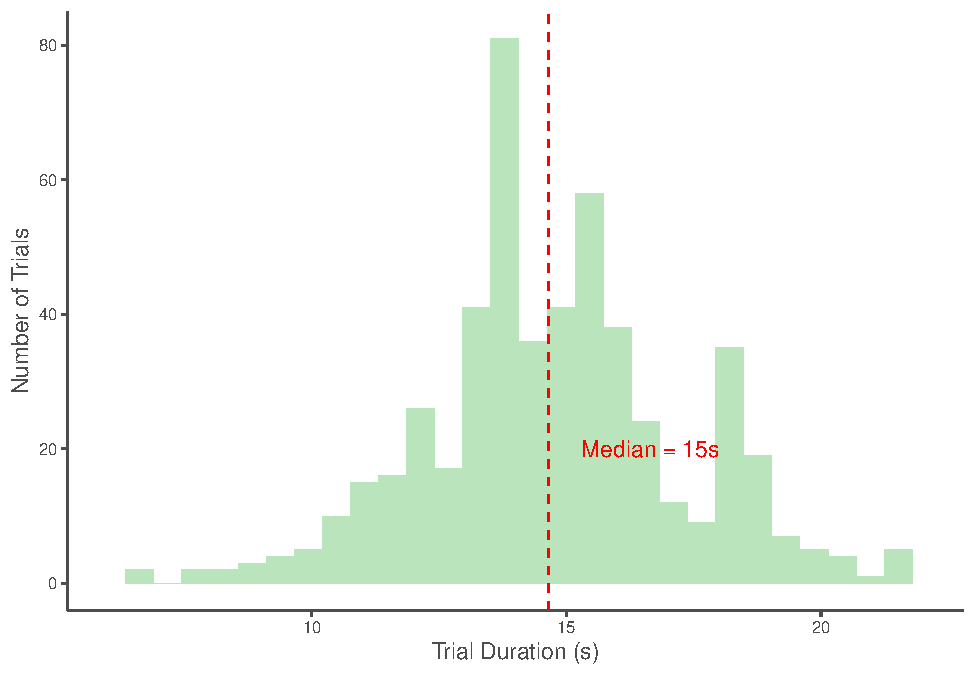
\includegraphics{revised_ms_analyses_files/figure-latex/r2-cn-durations-trial-1.pdf}

\begin{Shaded}
\begin{Highlighting}[]
\FunctionTok{ggsave}\NormalTok{(}\FunctionTok{here}\NormalTok{(}\StringTok{\textquotesingle{}supplement/plots/exp\_1/pdfs\textquotesingle{}}\NormalTok{, }\StringTok{\textquotesingle{}cn\_trialdur\_histogram.pdf\textquotesingle{}}\NormalTok{), }
       \AttributeTok{device=}\StringTok{\textquotesingle{}pdf\textquotesingle{}}\NormalTok{, }\AttributeTok{width=}\FloatTok{2.5}\NormalTok{, }\AttributeTok{height=}\FloatTok{1.5}\NormalTok{, }\AttributeTok{units=}\StringTok{\textquotesingle{}in\textquotesingle{}}\NormalTok{, }\AttributeTok{scale=}\FloatTok{2.5}\NormalTok{)}
\FunctionTok{ggsave}\NormalTok{(}\FunctionTok{here}\NormalTok{(}\StringTok{\textquotesingle{}supplement/plots/exp\_1/pngs\textquotesingle{}}\NormalTok{, }\StringTok{\textquotesingle{}cn\_trialdur\_histogram.png\textquotesingle{}}\NormalTok{), }
       \AttributeTok{device=}\StringTok{\textquotesingle{}png\textquotesingle{}}\NormalTok{, }\AttributeTok{width=}\FloatTok{2.5}\NormalTok{, }\AttributeTok{height=}\FloatTok{1.5}\NormalTok{, }\AttributeTok{units=}\StringTok{\textquotesingle{}in\textquotesingle{}}\NormalTok{, }\AttributeTok{scale=}\FloatTok{2.5}\NormalTok{)}
\end{Highlighting}
\end{Shaded}

\begin{Shaded}
\begin{Highlighting}[]
\NormalTok{CN\_MED\_TRIAL\_LOOKING\_S }\OtherTok{\textless{}{-}} \FunctionTok{median}\NormalTok{(}
\NormalTok{  cn\_fin}\SpecialCharTok{$}\NormalTok{totaltrialtime\_looking\_sum\_s)}
\NormalTok{CN\_MIN\_TRIAL\_LOOKING\_S }\OtherTok{\textless{}{-}} 
  \FunctionTok{min}\NormalTok{(cn\_fin}\SpecialCharTok{$}\NormalTok{totaltrialtime\_looking\_sum\_s)}
\NormalTok{CN\_MAX\_TRIAL\_LOOKING\_S }\OtherTok{\textless{}{-}} 
  \FunctionTok{max}\NormalTok{(cn\_fin}\SpecialCharTok{$}\NormalTok{totaltrialtime\_looking\_sum\_s)}
\NormalTok{CN\_MEAN\_TRIAL\_LOOKING\_S }\OtherTok{\textless{}{-}} 
  \FunctionTok{mean}\NormalTok{(cn\_fin}\SpecialCharTok{$}\NormalTok{totaltrialtime\_looking\_sum\_s)}
\NormalTok{CN\_CIL\_TRIAL\_LOOKING\_S }\OtherTok{\textless{}{-}}\NormalTok{ CN\_MEAN\_TRIAL\_LOOKING\_S }\SpecialCharTok{{-}} 
  \FunctionTok{ci.low}\NormalTok{(cn\_fin}\SpecialCharTok{$}\NormalTok{totaltrialtime\_looking\_sum\_s)}
\NormalTok{CN\_CIH\_TRIAL\_LOOKING\_S }\OtherTok{\textless{}{-}}\NormalTok{ CN\_MEAN\_TRIAL\_LOOKING\_S }\SpecialCharTok{+} 
  \FunctionTok{ci.high}\NormalTok{(cn\_fin}\SpecialCharTok{$}\NormalTok{totaltrialtime\_looking\_sum\_s)}

\FunctionTok{ggplot}\NormalTok{(cn\_fin, }\FunctionTok{aes}\NormalTok{(}\AttributeTok{x=}\NormalTok{totaltrialtime\_looking\_sum\_s)) }\SpecialCharTok{+}
  \FunctionTok{geom\_histogram}\NormalTok{(}\AttributeTok{fill=}\StringTok{\textquotesingle{}\#7bccc4\textquotesingle{}}\NormalTok{) }\SpecialCharTok{+}
\NormalTok{  sb.density.theme }\SpecialCharTok{+}
  \FunctionTok{geom\_vline}\NormalTok{(}\AttributeTok{xintercept=}\NormalTok{CN\_MED\_TRIAL\_LOOKING\_S, }
             \AttributeTok{color=}\StringTok{\textquotesingle{}red\textquotesingle{}}\NormalTok{, }\AttributeTok{lty=}\DecValTok{2}\NormalTok{) }\SpecialCharTok{+}
  \FunctionTok{xlim}\NormalTok{(}\DecValTok{2}\NormalTok{,}\DecValTok{14}\NormalTok{) }\SpecialCharTok{+}
  \FunctionTok{xlab}\NormalTok{(}\StringTok{\textquotesingle{}Total Looking Time Duration (s)\textquotesingle{}}\NormalTok{) }\SpecialCharTok{+}
  \FunctionTok{ylab}\NormalTok{(}\StringTok{\textquotesingle{}Number of Trials\textquotesingle{}}\NormalTok{) }\SpecialCharTok{+} 
  \FunctionTok{theme}\NormalTok{(}\AttributeTok{axis.title =} \FunctionTok{element\_text}\NormalTok{(}\AttributeTok{colour=}\StringTok{\textquotesingle{}gray30\textquotesingle{}}\NormalTok{, }\AttributeTok{size=}\DecValTok{11}\NormalTok{),}
        \AttributeTok{axis.text =} \FunctionTok{element\_text}\NormalTok{(}\AttributeTok{colour=}\StringTok{\textquotesingle{}gray30\textquotesingle{}}\NormalTok{, }\AttributeTok{size=}\DecValTok{11}\NormalTok{),}
        \AttributeTok{axis.ticks =} \FunctionTok{element\_line}\NormalTok{(}\AttributeTok{colour=}\StringTok{\textquotesingle{}gray30\textquotesingle{}}\NormalTok{),}
        \AttributeTok{plot.background =} \FunctionTok{element\_blank}\NormalTok{(),}
        \AttributeTok{panel.grid.major =} \FunctionTok{element\_blank}\NormalTok{(),}
        \AttributeTok{panel.grid.minor =} \FunctionTok{element\_blank}\NormalTok{(),}
        \AttributeTok{panel.border =} \FunctionTok{element\_blank}\NormalTok{(),}
        \AttributeTok{panel.background =} \FunctionTok{element\_blank}\NormalTok{(),}
        \AttributeTok{axis.line =} \FunctionTok{element\_line}\NormalTok{(}\AttributeTok{color =} \StringTok{\textquotesingle{}gray30\textquotesingle{}}\NormalTok{))  }\SpecialCharTok{+}
  \FunctionTok{annotate}\NormalTok{(}
    \StringTok{\textquotesingle{}text\textquotesingle{}}\NormalTok{, }\AttributeTok{label =} \StringTok{\textquotesingle{}Median = 6.8s\textquotesingle{}}\NormalTok{,}
    \AttributeTok{x =}\NormalTok{ CN\_MED\_TRIAL\_LOOKING\_S}\FloatTok{+1.5}\NormalTok{, }\AttributeTok{y =} \DecValTok{69}\NormalTok{, }\AttributeTok{size =} \DecValTok{4}\NormalTok{, }\AttributeTok{colour =} \StringTok{\textquotesingle{}red\textquotesingle{}}\NormalTok{)}
\end{Highlighting}
\end{Shaded}

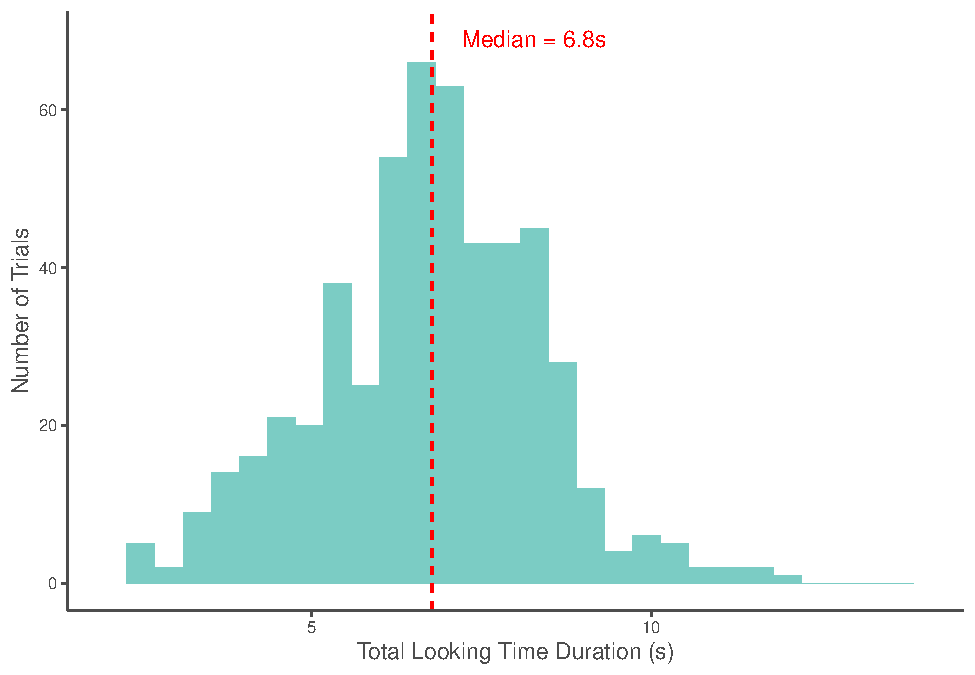
\includegraphics{revised_ms_analyses_files/figure-latex/r2-cn-durations-triallooking-1.pdf}

\begin{Shaded}
\begin{Highlighting}[]
\FunctionTok{ggsave}\NormalTok{(}\FunctionTok{here}\NormalTok{(}\StringTok{\textquotesingle{}supplement/plots/exp\_1/pdfs\textquotesingle{}}\NormalTok{, }\StringTok{\textquotesingle{}cn\_lookingtime\_histogram.pdf\textquotesingle{}}\NormalTok{), }
       \AttributeTok{device=}\StringTok{\textquotesingle{}pdf\textquotesingle{}}\NormalTok{, }\AttributeTok{width=}\FloatTok{2.5}\NormalTok{, }\AttributeTok{height=}\FloatTok{1.25}\NormalTok{, }\AttributeTok{units=}\StringTok{\textquotesingle{}in\textquotesingle{}}\NormalTok{, }\AttributeTok{scale=}\FloatTok{2.5}\NormalTok{)}
\FunctionTok{ggsave}\NormalTok{(}\FunctionTok{here}\NormalTok{(}\StringTok{\textquotesingle{}supplement/plots/exp\_1/pngs\textquotesingle{}}\NormalTok{, }\StringTok{\textquotesingle{}cn\_lookingtime\_histogram.png\textquotesingle{}}\NormalTok{),}
       \AttributeTok{device=}\StringTok{\textquotesingle{}png\textquotesingle{}}\NormalTok{, }\AttributeTok{width=}\FloatTok{2.5}\NormalTok{, }\AttributeTok{height=}\FloatTok{1.25}\NormalTok{, }\AttributeTok{units=}\StringTok{\textquotesingle{}in\textquotesingle{}}\NormalTok{, }\AttributeTok{scale=}\FloatTok{2.5}\NormalTok{)}
\end{Highlighting}
\end{Shaded}

\begin{Shaded}
\begin{Highlighting}[]
\NormalTok{CN\_MED\_LOOKING\_PROP }\OtherTok{\textless{}{-}} \FunctionTok{median}\NormalTok{(}
\NormalTok{  cn\_fin}\SpecialCharTok{$}\NormalTok{trialtolookingoffset\_prop)}
\NormalTok{CN\_MIN\_LOOKING\_PROP }\OtherTok{\textless{}{-}} \FunctionTok{min}\NormalTok{(}
\NormalTok{  cn\_fin}\SpecialCharTok{$}\NormalTok{trialtolookingoffset\_prop)}
\NormalTok{CN\_MAX\_LOOKING\_PROP }\OtherTok{\textless{}{-}} \FunctionTok{max}\NormalTok{(}
\NormalTok{  cn\_fin}\SpecialCharTok{$}\NormalTok{trialtolookingoffset\_prop)}
\NormalTok{CN\_MEAN\_LOOKING\_PROP }\OtherTok{\textless{}{-}} \FunctionTok{mean}\NormalTok{(}
\NormalTok{  cn\_fin}\SpecialCharTok{$}\NormalTok{trialtolookingoffset\_prop)}
\NormalTok{CN\_CIL\_LOOKING\_PROP }\OtherTok{\textless{}{-}}\NormalTok{ CN\_MEAN\_LOOKING\_PROP }\SpecialCharTok{{-}} \FunctionTok{ci.low}\NormalTok{(}
\NormalTok{  cn\_fin}\SpecialCharTok{$}\NormalTok{trialtolookingoffset\_prop)}
\NormalTok{CN\_CIH\_LOOKING\_PROP }\OtherTok{\textless{}{-}}\NormalTok{ CN\_MEAN\_LOOKING\_PROP }\SpecialCharTok{+}\FunctionTok{ci.high}\NormalTok{(}
\NormalTok{  cn\_fin}\SpecialCharTok{$}\NormalTok{trialtolookingoffset\_prop)}

\FunctionTok{ggplot}\NormalTok{(cn\_fin, }\FunctionTok{aes}\NormalTok{(}\AttributeTok{x=}\NormalTok{trialtolookingoffset\_prop)) }\SpecialCharTok{+}
  \FunctionTok{geom\_histogram}\NormalTok{(}\AttributeTok{fill=}\StringTok{\textquotesingle{}\#7bccc4\textquotesingle{}}\NormalTok{) }\SpecialCharTok{+}
\NormalTok{  sb.density.theme }\SpecialCharTok{+}
  \FunctionTok{geom\_vline}\NormalTok{(}\AttributeTok{xintercept=}\NormalTok{CN\_MED\_LOOKING\_PROP, }\AttributeTok{color=}\StringTok{\textquotesingle{}red\textquotesingle{}}\NormalTok{, }\AttributeTok{lty=}\DecValTok{2}\NormalTok{) }\SpecialCharTok{+}
  \FunctionTok{xlim}\NormalTok{(}\DecValTok{0}\NormalTok{,}\DecValTok{1}\NormalTok{) }\SpecialCharTok{+}
  \FunctionTok{xlab}\NormalTok{(}\StringTok{\textquotesingle{}Overall Looking Time Proportion\textquotesingle{}}\NormalTok{) }\SpecialCharTok{+}
  \FunctionTok{ylab}\NormalTok{(}\StringTok{\textquotesingle{}Number of Trials\textquotesingle{}}\NormalTok{) }\SpecialCharTok{+} 
  \FunctionTok{theme}\NormalTok{(}\AttributeTok{axis.title =} \FunctionTok{element\_text}\NormalTok{(}\AttributeTok{colour=}\StringTok{\textquotesingle{}gray30\textquotesingle{}}\NormalTok{, }\AttributeTok{size=}\DecValTok{11}\NormalTok{),}
        \AttributeTok{axis.text =} \FunctionTok{element\_text}\NormalTok{(}\AttributeTok{colour=}\StringTok{\textquotesingle{}gray30\textquotesingle{}}\NormalTok{, }\AttributeTok{size=}\DecValTok{11}\NormalTok{),}
        \AttributeTok{axis.ticks =} \FunctionTok{element\_line}\NormalTok{(}\AttributeTok{colour=}\StringTok{\textquotesingle{}gray30\textquotesingle{}}\NormalTok{),}
        \AttributeTok{plot.background =} \FunctionTok{element\_blank}\NormalTok{() ,}
        \AttributeTok{panel.grid.major =} \FunctionTok{element\_blank}\NormalTok{() ,}
        \AttributeTok{panel.grid.minor =} \FunctionTok{element\_blank}\NormalTok{() ,}
        \AttributeTok{panel.border =} \FunctionTok{element\_blank}\NormalTok{() ,}
        \AttributeTok{panel.background =} \FunctionTok{element\_blank}\NormalTok{(),}
        \AttributeTok{axis.line =} \FunctionTok{element\_line}\NormalTok{(}\AttributeTok{color =} \StringTok{\textquotesingle{}gray30\textquotesingle{}}\NormalTok{)) }\SpecialCharTok{+}
  \FunctionTok{annotate}\NormalTok{(}
    \StringTok{\textquotesingle{}text\textquotesingle{}}\NormalTok{, }\AttributeTok{label =} \StringTok{\textquotesingle{}Median = 0.47\textquotesingle{}}\NormalTok{,}
    \AttributeTok{x =}\NormalTok{ CN\_MED\_LOOKING\_PROP}\FloatTok{{-}.12}\NormalTok{, }\AttributeTok{y =} \DecValTok{68}\NormalTok{, }\AttributeTok{size =} \DecValTok{4}\NormalTok{, }\AttributeTok{colour =} \StringTok{\textquotesingle{}red\textquotesingle{}}\NormalTok{)}
\end{Highlighting}
\end{Shaded}

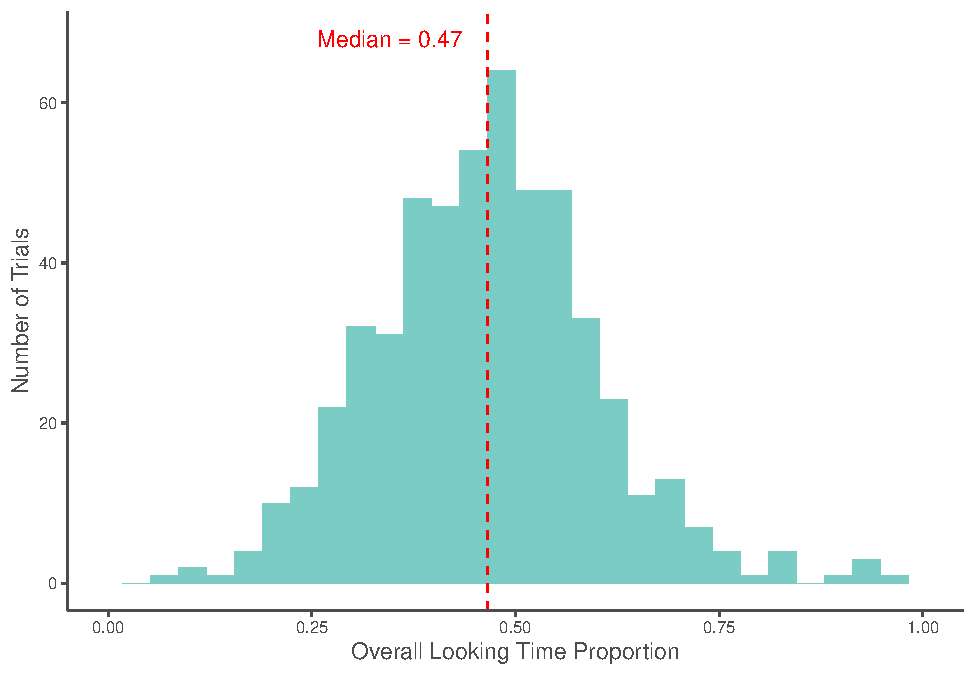
\includegraphics{revised_ms_analyses_files/figure-latex/r2-cn-durs-lookingprop-1.pdf}

\begin{Shaded}
\begin{Highlighting}[]
\FunctionTok{ggsave}\NormalTok{(}\FunctionTok{here}\NormalTok{(}\StringTok{\textquotesingle{}supplement/plots/exp\_1/pdfs\textquotesingle{}}\NormalTok{, }\StringTok{\textquotesingle{}cn\_lookingprop\_histogram.pdf\textquotesingle{}}\NormalTok{), }
       \AttributeTok{device=}\StringTok{\textquotesingle{}pdf\textquotesingle{}}\NormalTok{, }\AttributeTok{width=}\FloatTok{2.5}\NormalTok{, }\AttributeTok{height=}\FloatTok{1.25}\NormalTok{, }\AttributeTok{units=}\StringTok{\textquotesingle{}in\textquotesingle{}}\NormalTok{, }\AttributeTok{scale=}\FloatTok{2.5}\NormalTok{)}
\FunctionTok{ggsave}\NormalTok{(}\FunctionTok{here}\NormalTok{(}\StringTok{\textquotesingle{}supplement/plots/exp\_1/pngs\textquotesingle{}}\NormalTok{, }\StringTok{\textquotesingle{}cn\_lookingprop\_histogram.png\textquotesingle{}}\NormalTok{), }
       \AttributeTok{device=}\StringTok{\textquotesingle{}png\textquotesingle{}}\NormalTok{, }\AttributeTok{width=}\FloatTok{2.5}\NormalTok{, }\AttributeTok{height=}\FloatTok{1.25}\NormalTok{, }\AttributeTok{units=}\StringTok{\textquotesingle{}in\textquotesingle{}}\NormalTok{, }\AttributeTok{scale=}\FloatTok{2.5}\NormalTok{)}
\end{Highlighting}
\end{Shaded}

\begin{Shaded}
\begin{Highlighting}[]
\NormalTok{CN\_MED\_PRE\_DUR\_S }\OtherTok{\textless{}{-}} \FunctionTok{median}\NormalTok{(cn\_fin}\SpecialCharTok{$}\NormalTok{pre\_dur\_ms}\SpecialCharTok{/}\DecValTok{1000}\NormalTok{)}
\NormalTok{CN\_MIN\_PRE\_DUR\_S }\OtherTok{\textless{}{-}} \FunctionTok{min}\NormalTok{(cn\_fin}\SpecialCharTok{$}\NormalTok{pre\_dur\_ms}\SpecialCharTok{/}\DecValTok{1000}\NormalTok{)}
\NormalTok{CN\_MAX\_PRE\_DUR\_S }\OtherTok{\textless{}{-}} \FunctionTok{max}\NormalTok{(cn\_fin[cn\_fin}\SpecialCharTok{$}\NormalTok{pre\_dur\_ms}\SpecialCharTok{\textless{}}\DecValTok{10000}\NormalTok{,]}\SpecialCharTok{$}\NormalTok{pre\_dur\_ms}\SpecialCharTok{/}\DecValTok{1000}\NormalTok{)}
\NormalTok{CN\_MEAN\_PRE\_DUR\_S }\OtherTok{\textless{}{-}} \FunctionTok{mean}\NormalTok{(cn\_fin[cn\_fin}\SpecialCharTok{$}\NormalTok{pre\_dur\_ms}\SpecialCharTok{\textless{}}\DecValTok{10000}\NormalTok{,]}\SpecialCharTok{$}\NormalTok{pre\_dur\_ms}\SpecialCharTok{/}\DecValTok{1000}\NormalTok{)}

\FunctionTok{ggplot}\NormalTok{(cn\_fin, }\FunctionTok{aes}\NormalTok{(}\AttributeTok{x=}\NormalTok{pre\_dur\_ms}\SpecialCharTok{/}\DecValTok{1000}\NormalTok{))}\SpecialCharTok{+}
  \FunctionTok{geom\_histogram}\NormalTok{(}\AttributeTok{fill=}\StringTok{\textquotesingle{}\#bae4bc\textquotesingle{}}\NormalTok{) }\SpecialCharTok{+}
\NormalTok{  sb.density.theme }\SpecialCharTok{+}
  \FunctionTok{geom\_vline}\NormalTok{(}\AttributeTok{xintercept=}\NormalTok{CN\_MED\_PRE\_DUR\_S, }\AttributeTok{color=}\StringTok{\textquotesingle{}red\textquotesingle{}}\NormalTok{, }\AttributeTok{lty=}\DecValTok{2}\NormalTok{) }\SpecialCharTok{+}
  \CommentTok{\#geom\_vline(xintercept = 3.133, color=\textquotesingle{}red\textquotesingle{}) +}
  \FunctionTok{xlim}\NormalTok{(}\DecValTok{3}\NormalTok{,}\FloatTok{6.5}\NormalTok{)}\SpecialCharTok{+}
  \FunctionTok{xlab}\NormalTok{(}\StringTok{"\textquotesingle{}Pre{-}Naming\textquotesingle{} Window Duration (s)"}\NormalTok{) }\SpecialCharTok{+}
  \FunctionTok{ylab}\NormalTok{(}\StringTok{\textquotesingle{}Number of Trials\textquotesingle{}}\NormalTok{) }\SpecialCharTok{+} 
  \FunctionTok{theme}\NormalTok{(}\AttributeTok{axis.title =} \FunctionTok{element\_text}\NormalTok{(}\AttributeTok{colour=}\StringTok{\textquotesingle{}gray30\textquotesingle{}}\NormalTok{, }\AttributeTok{size=}\DecValTok{11}\NormalTok{),}
        \AttributeTok{axis.ticks =} \FunctionTok{element\_line}\NormalTok{(}\AttributeTok{colour=}\StringTok{\textquotesingle{}gray30\textquotesingle{}}\NormalTok{),}
        \AttributeTok{plot.background =} \FunctionTok{element\_blank}\NormalTok{() ,}
        \AttributeTok{panel.grid.major =} \FunctionTok{element\_blank}\NormalTok{() ,}
        \AttributeTok{panel.grid.minor =} \FunctionTok{element\_blank}\NormalTok{() ,}
        \AttributeTok{panel.border =} \FunctionTok{element\_blank}\NormalTok{() ,}
        \AttributeTok{panel.background =} \FunctionTok{element\_blank}\NormalTok{(),}
        \AttributeTok{axis.line =} \FunctionTok{element\_line}\NormalTok{(}\AttributeTok{color =} \StringTok{\textquotesingle{}gray30\textquotesingle{}}\NormalTok{)) }\SpecialCharTok{+}
  \FunctionTok{annotate}\NormalTok{(}
    \StringTok{\textquotesingle{}text\textquotesingle{}}\NormalTok{, }\AttributeTok{label =} \StringTok{\textquotesingle{}Median = 5s\textquotesingle{}}\NormalTok{,}
    \AttributeTok{x =}\NormalTok{ CN\_MED\_PRE\_DUR\_S}\FloatTok{+.4}\NormalTok{, }\AttributeTok{y =} \DecValTok{38}\NormalTok{, }\AttributeTok{size =} \DecValTok{4}\NormalTok{, }\AttributeTok{colour =} \StringTok{\textquotesingle{}red\textquotesingle{}}\NormalTok{)}
\end{Highlighting}
\end{Shaded}

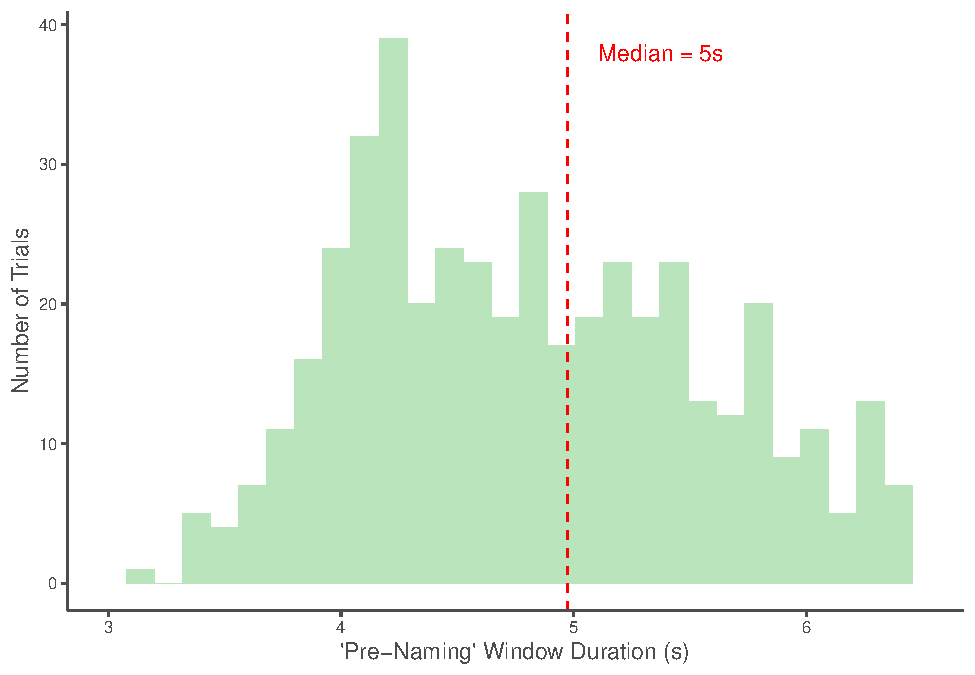
\includegraphics{revised_ms_analyses_files/figure-latex/r2-cn-pre-duration-1.pdf}

\begin{Shaded}
\begin{Highlighting}[]
\NormalTok{prelookingprop\_df }\OtherTok{\textless{}{-}}\NormalTok{ cn\_fin }\SpecialCharTok{\%\textgreater{}\%} 
  \FunctionTok{mutate}\NormalTok{(}\AttributeTok{window =} \StringTok{"\textquotesingle{}Pre{-}Naming\textquotesingle{} Window"}\NormalTok{,}
         \AttributeTok{looking\_prop =}\NormalTok{ pre\_looking\_sum\_ms}\SpecialCharTok{/}\NormalTok{pre\_dur\_ms,}
         \AttributeTok{median =} \FunctionTok{median}\NormalTok{(looking\_prop),}
         \AttributeTok{mean =} \FunctionTok{mean}\NormalTok{(looking\_prop)) }\SpecialCharTok{\%\textgreater{}\%}
\NormalTok{  dplyr}\SpecialCharTok{::}\FunctionTok{select}\NormalTok{(}\StringTok{\textquotesingle{}subject\_id\textquotesingle{}}\NormalTok{, }\StringTok{\textquotesingle{}window\textquotesingle{}}\NormalTok{, }\StringTok{\textquotesingle{}looking\_prop\textquotesingle{}}\NormalTok{, }\StringTok{\textquotesingle{}median\textquotesingle{}}\NormalTok{, }\StringTok{\textquotesingle{}mean\textquotesingle{}}\NormalTok{)}

\NormalTok{CN\_PRE\_MIN\_PROP }\OtherTok{\textless{}{-}} \FunctionTok{min}\NormalTok{(prelookingprop\_df}\SpecialCharTok{$}\NormalTok{looking\_prop)}
\NormalTok{CN\_PRE\_MAX\_PROP }\OtherTok{\textless{}{-}} \FunctionTok{max}\NormalTok{(prelookingprop\_df}\SpecialCharTok{$}\NormalTok{looking\_prop)}
\NormalTok{CN\_PRE\_MEAN\_PROP }\OtherTok{\textless{}{-}} \FunctionTok{mean}\NormalTok{(prelookingprop\_df}\SpecialCharTok{$}\NormalTok{looking\_prop)}
\NormalTok{CN\_PRE\_MEDIAN\_PROP }\OtherTok{\textless{}{-}} \FunctionTok{median}\NormalTok{(prelookingprop\_df}\SpecialCharTok{$}\NormalTok{looking\_prop)}

\NormalTok{postlookingprop\_df }\OtherTok{\textless{}{-}}\NormalTok{ cn\_fin }\SpecialCharTok{\%\textgreater{}\%} 
  \FunctionTok{mutate}\NormalTok{(}\AttributeTok{window =} \StringTok{"\textquotesingle{}Post{-}Naming\textquotesingle{}/Analysis Window"}\NormalTok{,}
         \AttributeTok{looking\_prop =}\NormalTok{ post1\_looking\_sum\_ms}\SpecialCharTok{/}\NormalTok{post1\_dur\_ms,}
         \AttributeTok{median =} \FunctionTok{median}\NormalTok{(looking\_prop),}
         \AttributeTok{mean =} \FunctionTok{mean}\NormalTok{(looking\_prop)) }\SpecialCharTok{\%\textgreater{}\%}
\NormalTok{  dplyr}\SpecialCharTok{::}\FunctionTok{select}\NormalTok{(}\StringTok{\textquotesingle{}subject\_id\textquotesingle{}}\NormalTok{, }\StringTok{\textquotesingle{}window\textquotesingle{}}\NormalTok{, }\StringTok{\textquotesingle{}looking\_prop\textquotesingle{}}\NormalTok{, }\StringTok{\textquotesingle{}median\textquotesingle{}}\NormalTok{, }\StringTok{\textquotesingle{}mean\textquotesingle{}}\NormalTok{)}

\NormalTok{CN\_POST\_MIN\_PROP }\OtherTok{\textless{}{-}} \FunctionTok{min}\NormalTok{(postlookingprop\_df}\SpecialCharTok{$}\NormalTok{looking\_prop)}
\NormalTok{CN\_POST\_MAX\_PROP }\OtherTok{\textless{}{-}} \FunctionTok{max}\NormalTok{(postlookingprop\_df}\SpecialCharTok{$}\NormalTok{looking\_prop)}
\NormalTok{CN\_POST\_MEAN\_PROP }\OtherTok{\textless{}{-}} \FunctionTok{mean}\NormalTok{(postlookingprop\_df}\SpecialCharTok{$}\NormalTok{looking\_prop)}
\NormalTok{CN\_POST\_MEDIAN\_PROP }\OtherTok{\textless{}{-}} \FunctionTok{median}\NormalTok{(postlookingprop\_df}\SpecialCharTok{$}\NormalTok{looking\_prop)}

\NormalTok{prepost\_lookingprop\_df }\OtherTok{\textless{}{-}} \FunctionTok{rbind}\NormalTok{(prelookingprop\_df, postlookingprop\_df)}
\NormalTok{prepost\_lookingprop\_df}\SpecialCharTok{$}\NormalTok{window }\OtherTok{\textless{}{-}} 
  \FunctionTok{factor}\NormalTok{(prepost\_lookingprop\_df}\SpecialCharTok{$}\NormalTok{window, }\AttributeTok{levels=}\FunctionTok{c}\NormalTok{(}
    \StringTok{"\textquotesingle{}Pre{-}Naming\textquotesingle{} Window"}\NormalTok{,}\StringTok{"\textquotesingle{}Post{-}Naming\textquotesingle{}/Analysis Window"}\NormalTok{), }\AttributeTok{ordered=}\NormalTok{T) }

\NormalTok{prepost\_lookingprop\_label\_df }\OtherTok{\textless{}{-}}\NormalTok{ prepost\_lookingprop\_df }\SpecialCharTok{\%\textgreater{}\%}
  \FunctionTok{group\_by}\NormalTok{(window) }\SpecialCharTok{\%\textgreater{}\%}
  \FunctionTok{summarize}\NormalTok{(}\AttributeTok{median=}\FunctionTok{median}\NormalTok{(median),}
            \AttributeTok{label=}\FunctionTok{paste}\NormalTok{(}\StringTok{\textquotesingle{}Median =\textquotesingle{}}\NormalTok{, }\FunctionTok{round}\NormalTok{(median, }\DecValTok{2}\NormalTok{), }\AttributeTok{sep=}\StringTok{\textquotesingle{} \textquotesingle{}}\NormalTok{))}

\FunctionTok{ggplot}\NormalTok{(prepost\_lookingprop\_df, }\FunctionTok{aes}\NormalTok{(}\AttributeTok{x=}\NormalTok{looking\_prop)) }\SpecialCharTok{+}
  \FunctionTok{geom\_histogram}\NormalTok{(}\AttributeTok{fill=}\StringTok{\textquotesingle{}\#7bccc4\textquotesingle{}}\NormalTok{) }\SpecialCharTok{+}
\NormalTok{  sb.density.theme }\SpecialCharTok{+}
  \FunctionTok{geom\_vline}\NormalTok{(}\FunctionTok{aes}\NormalTok{(}\AttributeTok{xintercept=}\NormalTok{median), }\AttributeTok{color=}\StringTok{\textquotesingle{}red\textquotesingle{}}\NormalTok{, }\AttributeTok{lty=}\DecValTok{2}\NormalTok{) }\SpecialCharTok{+}
  \FunctionTok{xlim}\NormalTok{(}\DecValTok{0}\NormalTok{,}\DecValTok{1}\NormalTok{) }\SpecialCharTok{+}
  \FunctionTok{ylim}\NormalTok{(}\DecValTok{0}\NormalTok{,}\DecValTok{100}\NormalTok{) }\SpecialCharTok{+}
  \FunctionTok{xlab}\NormalTok{(}\StringTok{\textquotesingle{}Looking Time Proportion\textquotesingle{}}\NormalTok{) }\SpecialCharTok{+}
  \FunctionTok{ylab}\NormalTok{(}\StringTok{\textquotesingle{}Number of Trials\textquotesingle{}}\NormalTok{) }\SpecialCharTok{+} 
  \FunctionTok{theme}\NormalTok{(}\AttributeTok{axis.title =} \FunctionTok{element\_text}\NormalTok{(}\AttributeTok{colour=}\StringTok{\textquotesingle{}gray30\textquotesingle{}}\NormalTok{, }\AttributeTok{size=}\DecValTok{11}\NormalTok{),}
        \AttributeTok{axis.text =} \FunctionTok{element\_text}\NormalTok{(}\AttributeTok{colour=}\StringTok{\textquotesingle{}gray30\textquotesingle{}}\NormalTok{, }\AttributeTok{size=}\DecValTok{11}\NormalTok{),}
        \AttributeTok{axis.ticks =} \FunctionTok{element\_line}\NormalTok{(}\AttributeTok{colour=}\StringTok{\textquotesingle{}gray30\textquotesingle{}}\NormalTok{),}
        \AttributeTok{plot.background =} \FunctionTok{element\_blank}\NormalTok{(),}
        \AttributeTok{strip.text.x =} \FunctionTok{element\_text}\NormalTok{(}\AttributeTok{colour=}\StringTok{\textquotesingle{}gray30\textquotesingle{}}\NormalTok{, }\AttributeTok{size=}\DecValTok{11}\NormalTok{))}\SpecialCharTok{+}
  \FunctionTok{facet\_wrap}\NormalTok{(}\SpecialCharTok{\textasciitilde{}}\NormalTok{window) }\SpecialCharTok{+}
  \FunctionTok{geom\_text}\NormalTok{(}\AttributeTok{data=}\NormalTok{prepost\_lookingprop\_label\_df,}
            \FunctionTok{aes}\NormalTok{(}\AttributeTok{x=}\NormalTok{median}\FloatTok{{-}.24}\NormalTok{, }\AttributeTok{label=}\NormalTok{label), }\AttributeTok{y=}\DecValTok{21}\NormalTok{, }
            \AttributeTok{color=}\StringTok{\textquotesingle{}red\textquotesingle{}}\NormalTok{, }\AttributeTok{size=}\DecValTok{4}\NormalTok{)}
\end{Highlighting}
\end{Shaded}

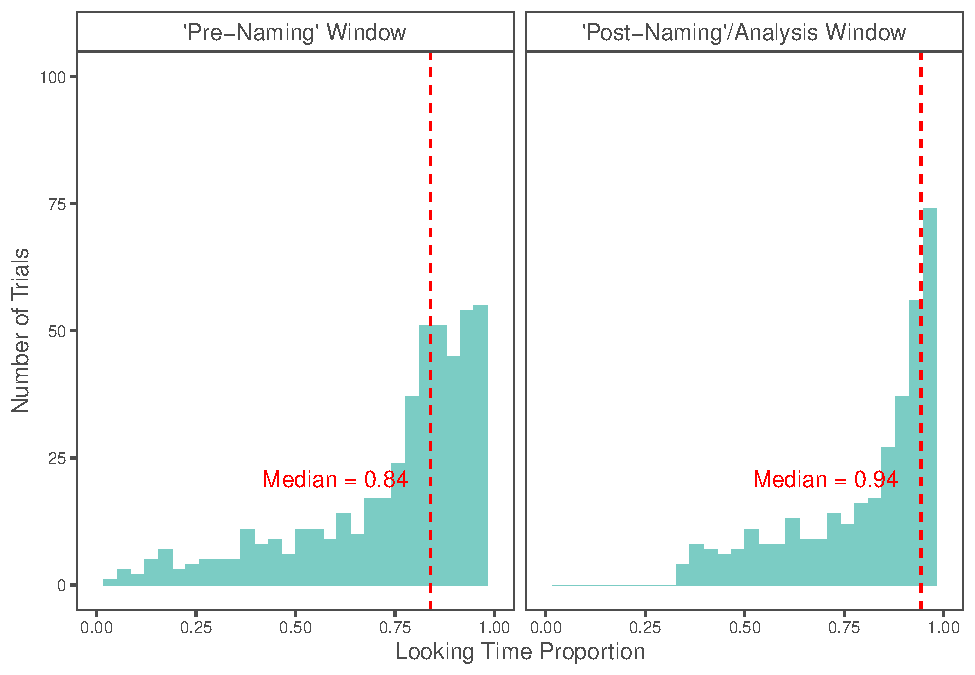
\includegraphics{revised_ms_analyses_files/figure-latex/r2-cn-durs-prepost-lookingprops-1.pdf}

\begin{Shaded}
\begin{Highlighting}[]
\FunctionTok{ggsave}\NormalTok{(}\FunctionTok{here}\NormalTok{(}\StringTok{\textquotesingle{}supplement/plots/exp\_1/pdfs\textquotesingle{}}\NormalTok{, }\StringTok{\textquotesingle{}cn\_lookingprops\_prepost.pdf\textquotesingle{}}\NormalTok{), }
       \AttributeTok{device=}\StringTok{\textquotesingle{}pdf\textquotesingle{}}\NormalTok{, }\AttributeTok{width=}\FloatTok{2.75}\NormalTok{, }\AttributeTok{height=}\FloatTok{1.5}\NormalTok{, }\AttributeTok{units=}\StringTok{\textquotesingle{}in\textquotesingle{}}\NormalTok{, }\AttributeTok{scale=}\FloatTok{2.5}\NormalTok{)}
\FunctionTok{ggsave}\NormalTok{(}\FunctionTok{here}\NormalTok{(}\StringTok{\textquotesingle{}supplement/plots/exp\_1/pngs\textquotesingle{}}\NormalTok{, }\StringTok{\textquotesingle{}cn\_lookingprops\_prepost.png\textquotesingle{}}\NormalTok{), }
       \AttributeTok{device=}\StringTok{\textquotesingle{}png\textquotesingle{}}\NormalTok{, }\AttributeTok{width=}\FloatTok{2.75}\NormalTok{, }\AttributeTok{height=}\FloatTok{1.5}\NormalTok{, }\AttributeTok{units=}\StringTok{\textquotesingle{}in\textquotesingle{}}\NormalTok{, }\AttributeTok{scale=}\FloatTok{2.5}\NormalTok{)}
\end{Highlighting}
\end{Shaded}

\begin{Shaded}
\begin{Highlighting}[]
\NormalTok{prelookingdur\_df }\OtherTok{\textless{}{-}}\NormalTok{ cn\_fin }\SpecialCharTok{\%\textgreater{}\%} 
  \FunctionTok{mutate}\NormalTok{(}\AttributeTok{window =} \StringTok{"\textquotesingle{}Pre{-}Naming\textquotesingle{} Window"}\NormalTok{,}
         \AttributeTok{looking\_dur =}\NormalTok{ pre\_looking\_sum\_ms}\SpecialCharTok{/}\DecValTok{1000}\NormalTok{,}
         \AttributeTok{median =} \FunctionTok{median}\NormalTok{(looking\_dur),}
         \AttributeTok{mean =} \FunctionTok{mean}\NormalTok{(looking\_dur)) }\SpecialCharTok{\%\textgreater{}\%}
\NormalTok{  dplyr}\SpecialCharTok{::}\FunctionTok{select}\NormalTok{(}\StringTok{\textquotesingle{}subject\_id\textquotesingle{}}\NormalTok{, }\StringTok{\textquotesingle{}window\textquotesingle{}}\NormalTok{, }\StringTok{\textquotesingle{}looking\_dur\textquotesingle{}}\NormalTok{, }\StringTok{\textquotesingle{}median\textquotesingle{}}\NormalTok{, }\StringTok{\textquotesingle{}mean\textquotesingle{}}\NormalTok{)}

\NormalTok{CN\_PRE\_MIN\_DUR }\OtherTok{\textless{}{-}} \FunctionTok{min}\NormalTok{(prelookingdur\_df}\SpecialCharTok{$}\NormalTok{pre\_looking\_sum\_ms)}
\NormalTok{CN\_PRE\_MAX\_DUR }\OtherTok{\textless{}{-}} \FunctionTok{max}\NormalTok{(prelookingdur\_df}\SpecialCharTok{$}\NormalTok{pre\_looking\_sum\_ms)}
\NormalTok{CN\_PRE\_MEAN\_DUR }\OtherTok{\textless{}{-}} \FunctionTok{mean}\NormalTok{(prelookingdur\_df}\SpecialCharTok{$}\NormalTok{pre\_looking\_sum\_ms)}
\NormalTok{CN\_PRE\_MEDIAN\_DUR }\OtherTok{\textless{}{-}} \FunctionTok{median}\NormalTok{(prelookingdur\_df}\SpecialCharTok{$}\NormalTok{pre\_looking\_sum\_ms)}

\NormalTok{postlookingdur\_df }\OtherTok{\textless{}{-}}\NormalTok{ cn\_fin }\SpecialCharTok{\%\textgreater{}\%} 
  \FunctionTok{mutate}\NormalTok{(}\AttributeTok{window =} \StringTok{"\textquotesingle{}Post{-}Naming\textquotesingle{}/Analysis Window"}\NormalTok{,}
         \AttributeTok{looking\_dur =}\NormalTok{ post1\_looking\_sum\_ms}\SpecialCharTok{/}\DecValTok{1000}\NormalTok{,}
         \AttributeTok{median =} \FunctionTok{median}\NormalTok{(looking\_dur),}
         \AttributeTok{mean =} \FunctionTok{mean}\NormalTok{(looking\_dur)) }\SpecialCharTok{\%\textgreater{}\%}
\NormalTok{  dplyr}\SpecialCharTok{::}\FunctionTok{select}\NormalTok{(}\StringTok{\textquotesingle{}subject\_id\textquotesingle{}}\NormalTok{, }\StringTok{\textquotesingle{}window\textquotesingle{}}\NormalTok{, }\StringTok{\textquotesingle{}looking\_dur\textquotesingle{}}\NormalTok{, }\StringTok{\textquotesingle{}median\textquotesingle{}}\NormalTok{, }\StringTok{\textquotesingle{}mean\textquotesingle{}}\NormalTok{)}

\NormalTok{CN\_POST\_MIN\_DUR }\OtherTok{\textless{}{-}} \FunctionTok{min}\NormalTok{(postlookingdur\_df}\SpecialCharTok{$}\NormalTok{looking\_dur)}
\NormalTok{CN\_POST\_MAX\_DUR }\OtherTok{\textless{}{-}} \FunctionTok{max}\NormalTok{(postlookingdur\_df}\SpecialCharTok{$}\NormalTok{looking\_dur)}
\NormalTok{CN\_POST\_MEAN\_DUR }\OtherTok{\textless{}{-}} \FunctionTok{mean}\NormalTok{(postlookingdur\_df}\SpecialCharTok{$}\NormalTok{looking\_dur)}
\NormalTok{CN\_POST\_MEDIAN\_DUR }\OtherTok{\textless{}{-}} \FunctionTok{median}\NormalTok{(postlookingdur\_df}\SpecialCharTok{$}\NormalTok{looking\_dur)}

\NormalTok{prepost\_lookingdur\_df }\OtherTok{\textless{}{-}} \FunctionTok{rbind}\NormalTok{(prelookingdur\_df, postlookingdur\_df)}
\NormalTok{prepost\_lookingdur\_df}\SpecialCharTok{$}\NormalTok{window }\OtherTok{\textless{}{-}} 
  \FunctionTok{factor}\NormalTok{(prepost\_lookingdur\_df}\SpecialCharTok{$}\NormalTok{window, }\AttributeTok{levels=}\FunctionTok{c}\NormalTok{(}
    \StringTok{"\textquotesingle{}Pre{-}Naming\textquotesingle{} Window"}\NormalTok{,}\StringTok{"\textquotesingle{}Post{-}Naming\textquotesingle{}/Analysis Window"}\NormalTok{), }\AttributeTok{ordered=}\NormalTok{T) }

\NormalTok{prepost\_lookingdur\_label\_df }\OtherTok{\textless{}{-}}\NormalTok{ prepost\_lookingdur\_df }\SpecialCharTok{\%\textgreater{}\%}
  \FunctionTok{group\_by}\NormalTok{(window) }\SpecialCharTok{\%\textgreater{}\%}
  \FunctionTok{summarize}\NormalTok{(}\AttributeTok{median=}\FunctionTok{median}\NormalTok{(median),}
            \AttributeTok{label=}\FunctionTok{paste}\NormalTok{(}\StringTok{\textquotesingle{}Median =\textquotesingle{}}\NormalTok{, }\FunctionTok{round}\NormalTok{(median, }\DecValTok{2}\NormalTok{), }\AttributeTok{sep=}\StringTok{\textquotesingle{} \textquotesingle{}}\NormalTok{))}

\NormalTok{cn\_pp\_durs }\OtherTok{\textless{}{-}} \FunctionTok{ggplot}\NormalTok{(prepost\_lookingdur\_df, }\FunctionTok{aes}\NormalTok{(}\AttributeTok{x=}\NormalTok{looking\_dur)) }\SpecialCharTok{+}
  \FunctionTok{geom\_histogram}\NormalTok{(}\AttributeTok{fill=}\StringTok{\textquotesingle{}\#7bccc4\textquotesingle{}}\NormalTok{) }\SpecialCharTok{+}
\NormalTok{  sb.density.theme }\SpecialCharTok{+}
  \FunctionTok{geom\_vline}\NormalTok{(}\FunctionTok{aes}\NormalTok{(}\AttributeTok{xintercept=}\NormalTok{median), }\AttributeTok{color=}\StringTok{\textquotesingle{}red\textquotesingle{}}\NormalTok{, }\AttributeTok{lty=}\DecValTok{2}\NormalTok{) }\SpecialCharTok{+}
  \FunctionTok{xlim}\NormalTok{(}\DecValTok{0}\NormalTok{,}\DecValTok{9}\NormalTok{) }\SpecialCharTok{+}
  \CommentTok{\#ylim(0,100) +}
  \FunctionTok{xlab}\NormalTok{(}\StringTok{\textquotesingle{}Looking Time Duration (s)\textquotesingle{}}\NormalTok{) }\SpecialCharTok{+}
  \FunctionTok{ylab}\NormalTok{(}\StringTok{\textquotesingle{}Number of Trials\textquotesingle{}}\NormalTok{) }\SpecialCharTok{+} 
  \FunctionTok{theme}\NormalTok{(}\AttributeTok{axis.title =} \FunctionTok{element\_text}\NormalTok{(}\AttributeTok{colour=}\StringTok{\textquotesingle{}gray30\textquotesingle{}}\NormalTok{, }\AttributeTok{size=}\DecValTok{11}\NormalTok{),}
        \AttributeTok{axis.text =} \FunctionTok{element\_text}\NormalTok{(}\AttributeTok{colour=}\StringTok{\textquotesingle{}gray30\textquotesingle{}}\NormalTok{, }\AttributeTok{size=}\DecValTok{11}\NormalTok{),}
        \AttributeTok{axis.ticks =} \FunctionTok{element\_line}\NormalTok{(}\AttributeTok{colour=}\StringTok{\textquotesingle{}gray30\textquotesingle{}}\NormalTok{),}
        \AttributeTok{plot.background =} \FunctionTok{element\_blank}\NormalTok{(),}
        \AttributeTok{strip.text.x =} \FunctionTok{element\_text}\NormalTok{(}\AttributeTok{colour=}\StringTok{\textquotesingle{}gray30\textquotesingle{}}\NormalTok{, }\AttributeTok{size=}\DecValTok{11}\NormalTok{))}\SpecialCharTok{+}
  \FunctionTok{facet\_wrap}\NormalTok{(}\SpecialCharTok{\textasciitilde{}}\NormalTok{window) }\SpecialCharTok{+}
  \FunctionTok{geom\_text}\NormalTok{(}\AttributeTok{data=}\NormalTok{prepost\_lookingdur\_label\_df,}
            \FunctionTok{aes}\NormalTok{(}\AttributeTok{x=}\NormalTok{median}\SpecialCharTok{+}\DecValTok{2}\NormalTok{, }\AttributeTok{label=}\NormalTok{label), }\AttributeTok{y=}\DecValTok{250}\NormalTok{, }
            \AttributeTok{color=}\StringTok{\textquotesingle{}red\textquotesingle{}}\NormalTok{, }\AttributeTok{size=}\DecValTok{4}\NormalTok{)}

\FunctionTok{ggsave}\NormalTok{(}\FunctionTok{here}\NormalTok{(}\StringTok{\textquotesingle{}supplement/plots/exp\_1/pdfs\textquotesingle{}}\NormalTok{, }\StringTok{\textquotesingle{}cn\_lookingdurs\_prepost.pdf\textquotesingle{}}\NormalTok{), }
       \AttributeTok{device=}\StringTok{\textquotesingle{}pdf\textquotesingle{}}\NormalTok{, }\AttributeTok{width=}\FloatTok{2.75}\NormalTok{, }\AttributeTok{height=}\FloatTok{1.5}\NormalTok{, }\AttributeTok{units=}\StringTok{\textquotesingle{}in\textquotesingle{}}\NormalTok{, }\AttributeTok{scale=}\FloatTok{2.5}\NormalTok{)}
\FunctionTok{ggsave}\NormalTok{(}\FunctionTok{here}\NormalTok{(}\StringTok{\textquotesingle{}supplement/plots/exp\_1/pngs\textquotesingle{}}\NormalTok{, }\StringTok{\textquotesingle{}cn\_lookingdurs\_prepost.png\textquotesingle{}}\NormalTok{), }
       \AttributeTok{device=}\StringTok{\textquotesingle{}png\textquotesingle{}}\NormalTok{, }\AttributeTok{width=}\FloatTok{2.75}\NormalTok{, }\AttributeTok{height=}\FloatTok{1.5}\NormalTok{, }\AttributeTok{units=}\StringTok{\textquotesingle{}in\textquotesingle{}}\NormalTok{, }\AttributeTok{scale=}\FloatTok{2.5}\NormalTok{)}
\end{Highlighting}
\end{Shaded}

Trials in Experiment 1 were \(14.86\)\textit{s} {[}\(14.60\), \(15.13\){]} long on average (\textit{range}: \(5.42-24.82\)\textit{s}, \(M_\textnormal{dur}=14.86\)\textit{s}, \textit{Med}\(=14.65\)\textit{s}), and infants spent an average of \(6.70\)\textit{s} {[}\(6.55\), \(6.84\){]} total looking at the displays (\textit{range}: \(1.97-12.17\)\textit{s}, \textit{Med}\(=6.77\)\textit{s}, or between \(0.07\) and \(0.99\) of the total trial duration; \(M=0.46\) {[}\(0.45\), \(0.48\){]}).

The pre-naming window was between \(3.12\) and \(9.44\)\textit{s} (\(M=5.22\)\textit{s}, \textit{Med}\(=4.97\)\textit{s}).

The children in our final sample spent similar proportions of time looking at the displays during the pre- and post-naming periods (\textsc{pre-naming} \textit{range}: \(0.03-1\), \(M=0.77\), \textit{Med}\(=0.84\); \textsc{post-naming} \textit{range}: \(0.34-1\), \(M=0.87\), \textit{Med}\(=0.94\)).


\end{document}
